\documentclass[letterpaper,12pt]{article}
\usepackage[left=1in,right=1in,top=1in,bottom=1in]{geometry}
\usepackage{amsmath,amssymb,mathtools}
\usepackage{accents}
\usepackage{lipsum}
\usepackage{longtable}

% so there will be a TOC in evince -- but where is it?
\usepackage{hyperref}

\newcommand{\bbR}{\mathbb{R}}
\newcommand{\bbC}{\mathbb{C}}
\newcommand{\ve}{\varepsilon}
\newcommand{\flipud}[1]{\operatorname{flipud}(#1)}
\newcommand{\fliplr}[1]{\operatorname{fliplr}(#1)}
\newcommand{\tE}{\tilde{E}_3}
\newcommand{\doublehat}[1]{\hat{\vphantom{\rule{1pt}{6.5pt}}\smash{\hat{#1}}}}
\newcommand{\inc}{\psi_{\text{inc}}}
\newcommand{\scatt}{\psi_{\text{scatt}}}
\newcommand{\diag}{\operatorname{diag}}
\newcommand{\dirA}{A^{(\text{Dir})}}
\newcommand{\pmlA}{A^{(\text{PML})}}
\newcommand{\dtnA}{A^{(\text{DtN})}}
\newcommand{\ratA}{A^{(\text{rat})}}
\newcommand{\dirB}{B^{(\text{Dir})}}
\newcommand{\pmlB}{B^{(\text{PML})}}
\newcommand{\dtnB}{B^{(\text{DtN})}}
\newcommand{\ratB}{B^{(\text{rat})}}
\newcommand{\dirT}{T^{(\text{Dir})}}
\newcommand{\pmlT}{T^{(\text{PML})}}
\newcommand{\dtnT}{T^{(\text{DtN})}}
\newcommand{\ratT}{T^{(\text{rat})}}
\newcommand{\pmlC}{C^{(\text{PML})}}
\newcommand{\dtnC}{C^{(\text{DtN})}}
\newcommand{\ratC}{C^{(\text{rat})}}
\newcommand{\Dtt}{D_{\theta\theta}}
\newcommand{\zn}[1]{\hat{z}^{(#1)}}
\newcommand{\wn}[1]{\hat{w}^{(#1)}}
\renewcommand{\H}{H_n^{(1)}(z)}
\renewcommand{\vec}{\operatorname{vec}}

\begin{document}

% title page
\title{ScattRes2D User's Guide}
\author{A. Hood}

\maketitle
\tableofcontents

\section{Introduction}
\label{sec-intro}

The code is for quantum scattering and resonance computation
for a class compactly-supported potentials.
In addition to being supported
in some disc $B(0,R)$, the potential $V$ must be smooth except possibly
on a finite number of circles $r = r_0$. For 
incident wave $\inc(r,\theta) = e^{ikr\cos\theta}$ with frequency
parameter $k$, the corresponding scattered wave obeys the equation
\begin{equation}\label{eqtn-scattprob}
\begin{aligned}
 \left(-\Delta + V - k^2\right)\scatt = -V\inc
 \qquad
 \text{on }B(0,R), \\ 
 \text{$\scatt$ outgoing}
 \qquad
 \text{on }\partial B(0,R).
\end{aligned}
\end{equation}
The boundary condition is enforced exactly with the Dirichlet-to-Neumann
(DtN)
map, approximately with a PML, and Dirichlet boundary conditions
work pretty well under special circumstances. Therefore, the user
can choose any of the three in order to compute $\scatt$.
The energy of the scattered wave is $E = k^2$.

The resonances are defined as the energies $E$ such that
\begin{equation}\label{eqtn-resprob}
\begin{aligned}
 \left(-\Delta + V - k^2\right)\scatt = 0
 \qquad
 \text{on }B(0,R), \\
 \text{$\scatt$ outgoing on }\partial B(0,R)
\end{aligned}
\end{equation}
has a nonzero solution. The user can still use Dirichlet boundary conditions
or a PML to enforce that the scattered wave is outgoing. 
It should be noted that we won't use the
DtN map for resonance computation, because the 
resulting eigenvalue problem is nonlinear (and non-polynomial and
non-rational). The user can choose to use a {\it rational approximation}
to the DtN map instead (which leads to a rational eigenvalue problem).



\section{The mesh}
\label{sec-mesh}

The scattered wave returned to the user is represented by its
values on a user-specified mesh, which we show here.
The mesh in the radial direction is specified piecewise, with
a half Chebyshev mesh on the inner disk (to avoid redundant density
at the center) and a normal Chebyshev mesh on other annular regions
(if any). 

\begin{figure}[h]
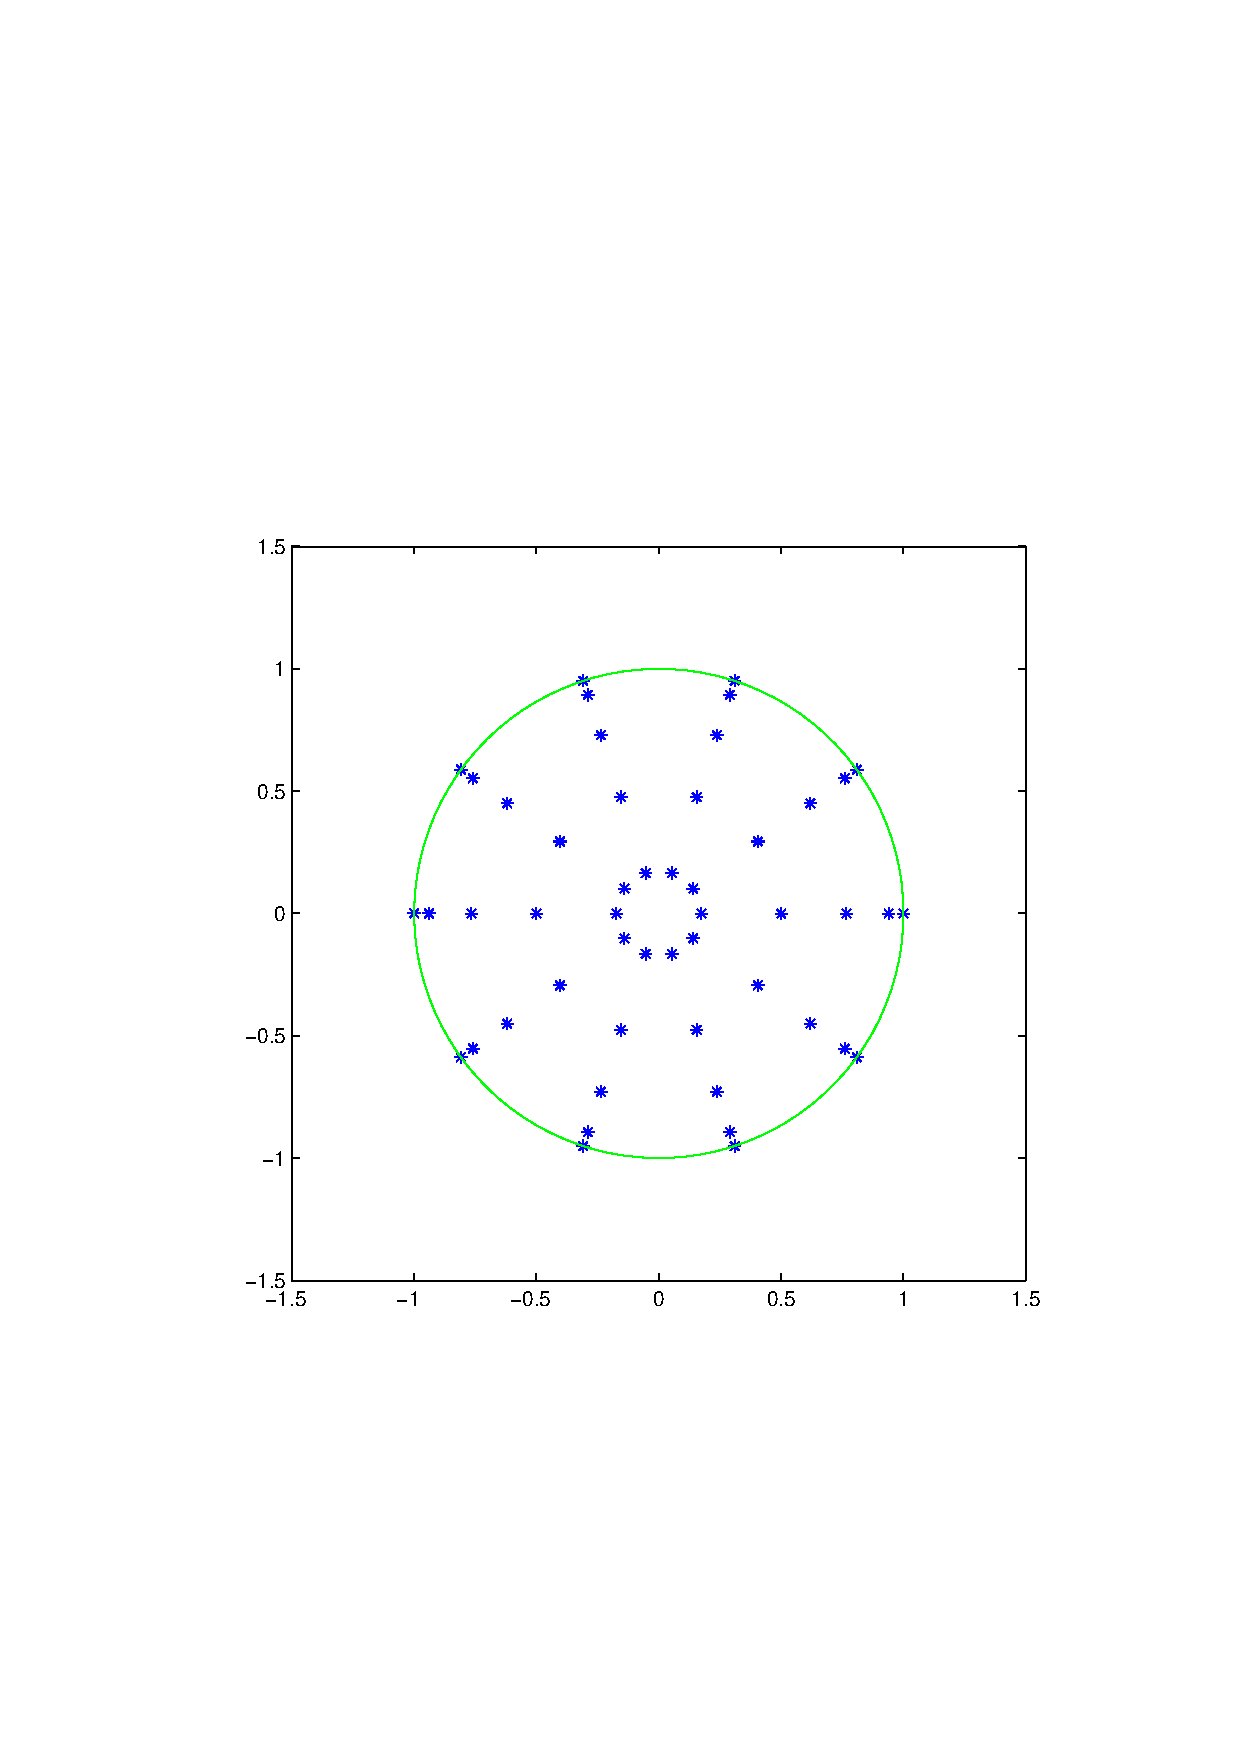
\includegraphics[width=0.49\linewidth]{figures/simplemesh.pdf}
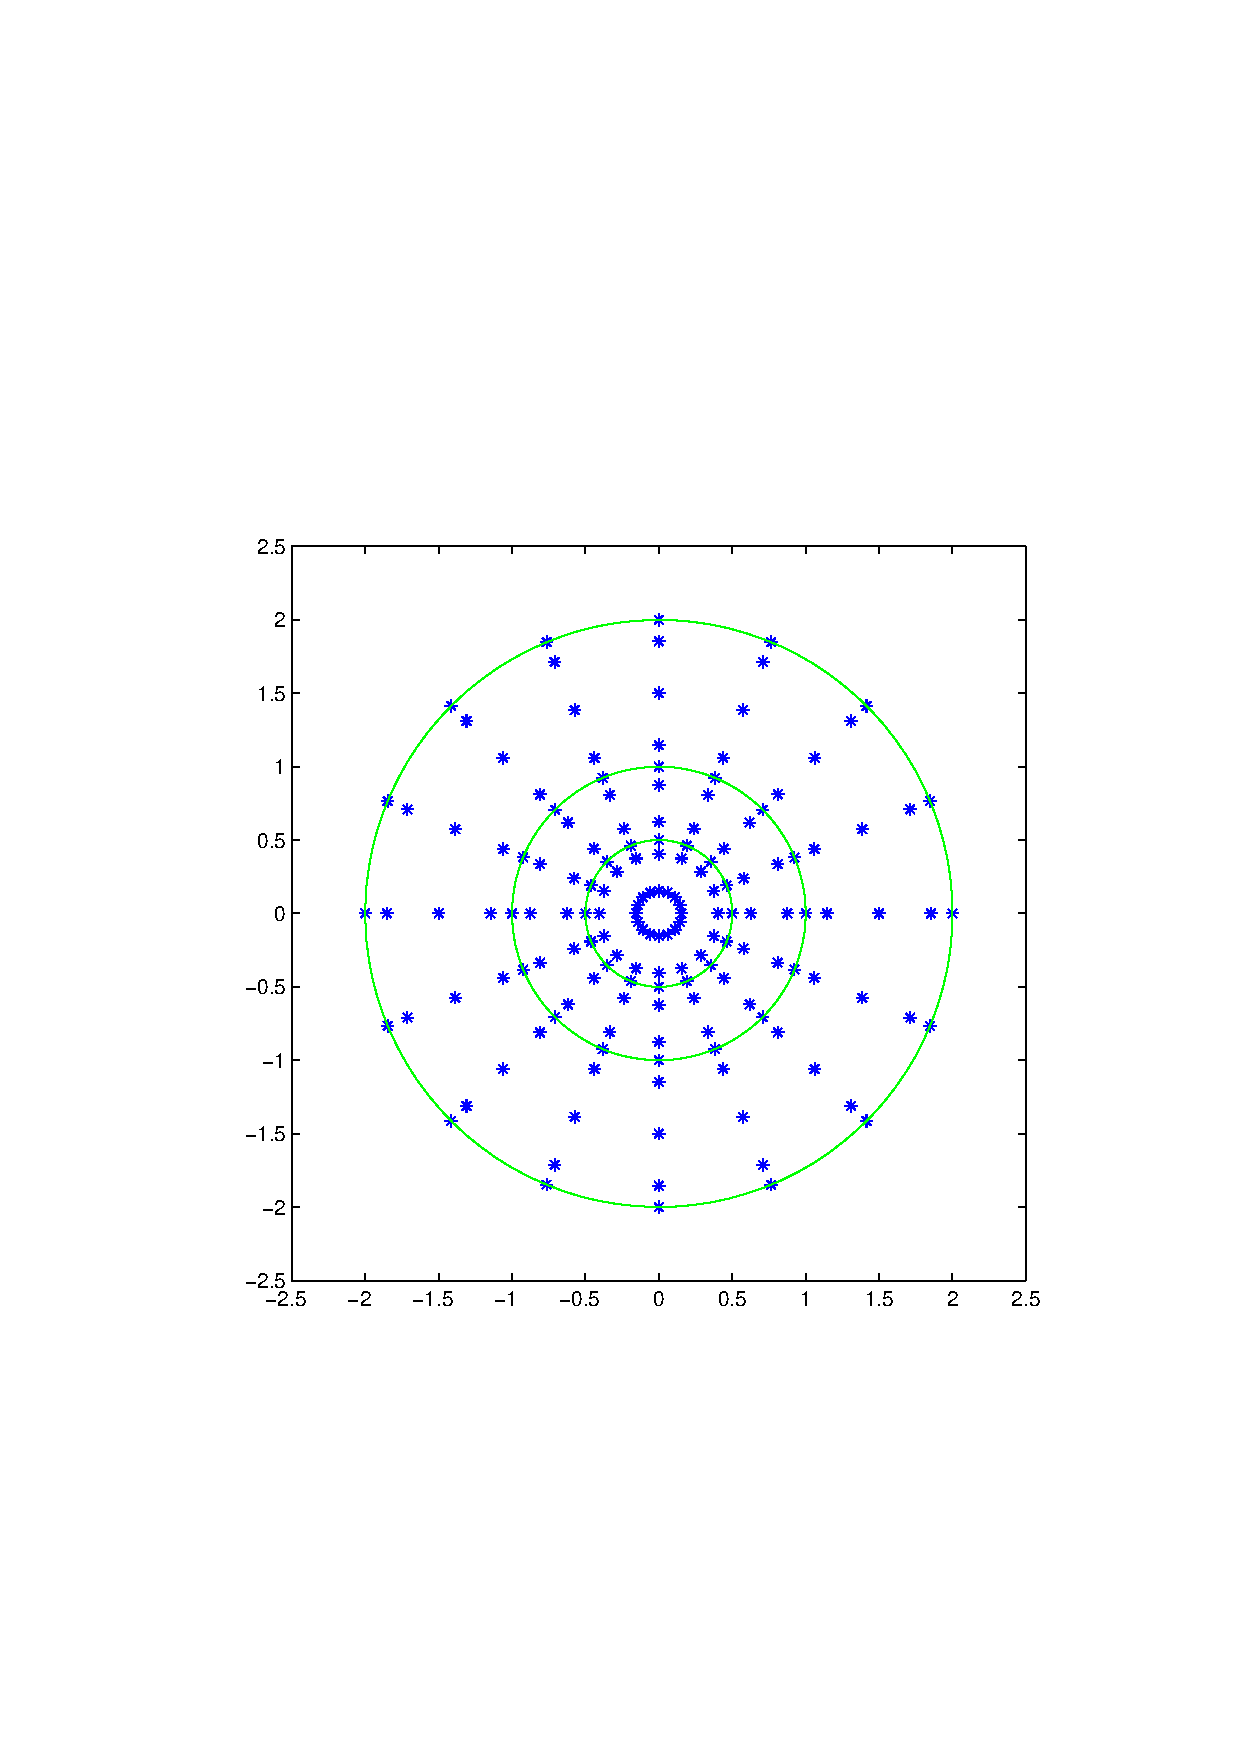
\includegraphics[width=0.49\linewidth]{figures/complicatedmesh.pdf}
\caption{Left: $R = 1$, eight $\theta$ mesh points ($N_t = 10$), 
               five points in half-Chebyshev mesh in radial 
               direction ($N_r = 5$).
         Right: Mesh specified piecewise, separately on
               $0 \le r \le 0.5$, $0.5 \le r \le 1$, and
               $1 \le r \le 2$.}
\end{figure}



\break
\section{The potential}
\label{sec-potential}

You can specify a potential in rectangular, polar, or complex
coordinates. Here are some examples.

\begin{figure}[h!]
 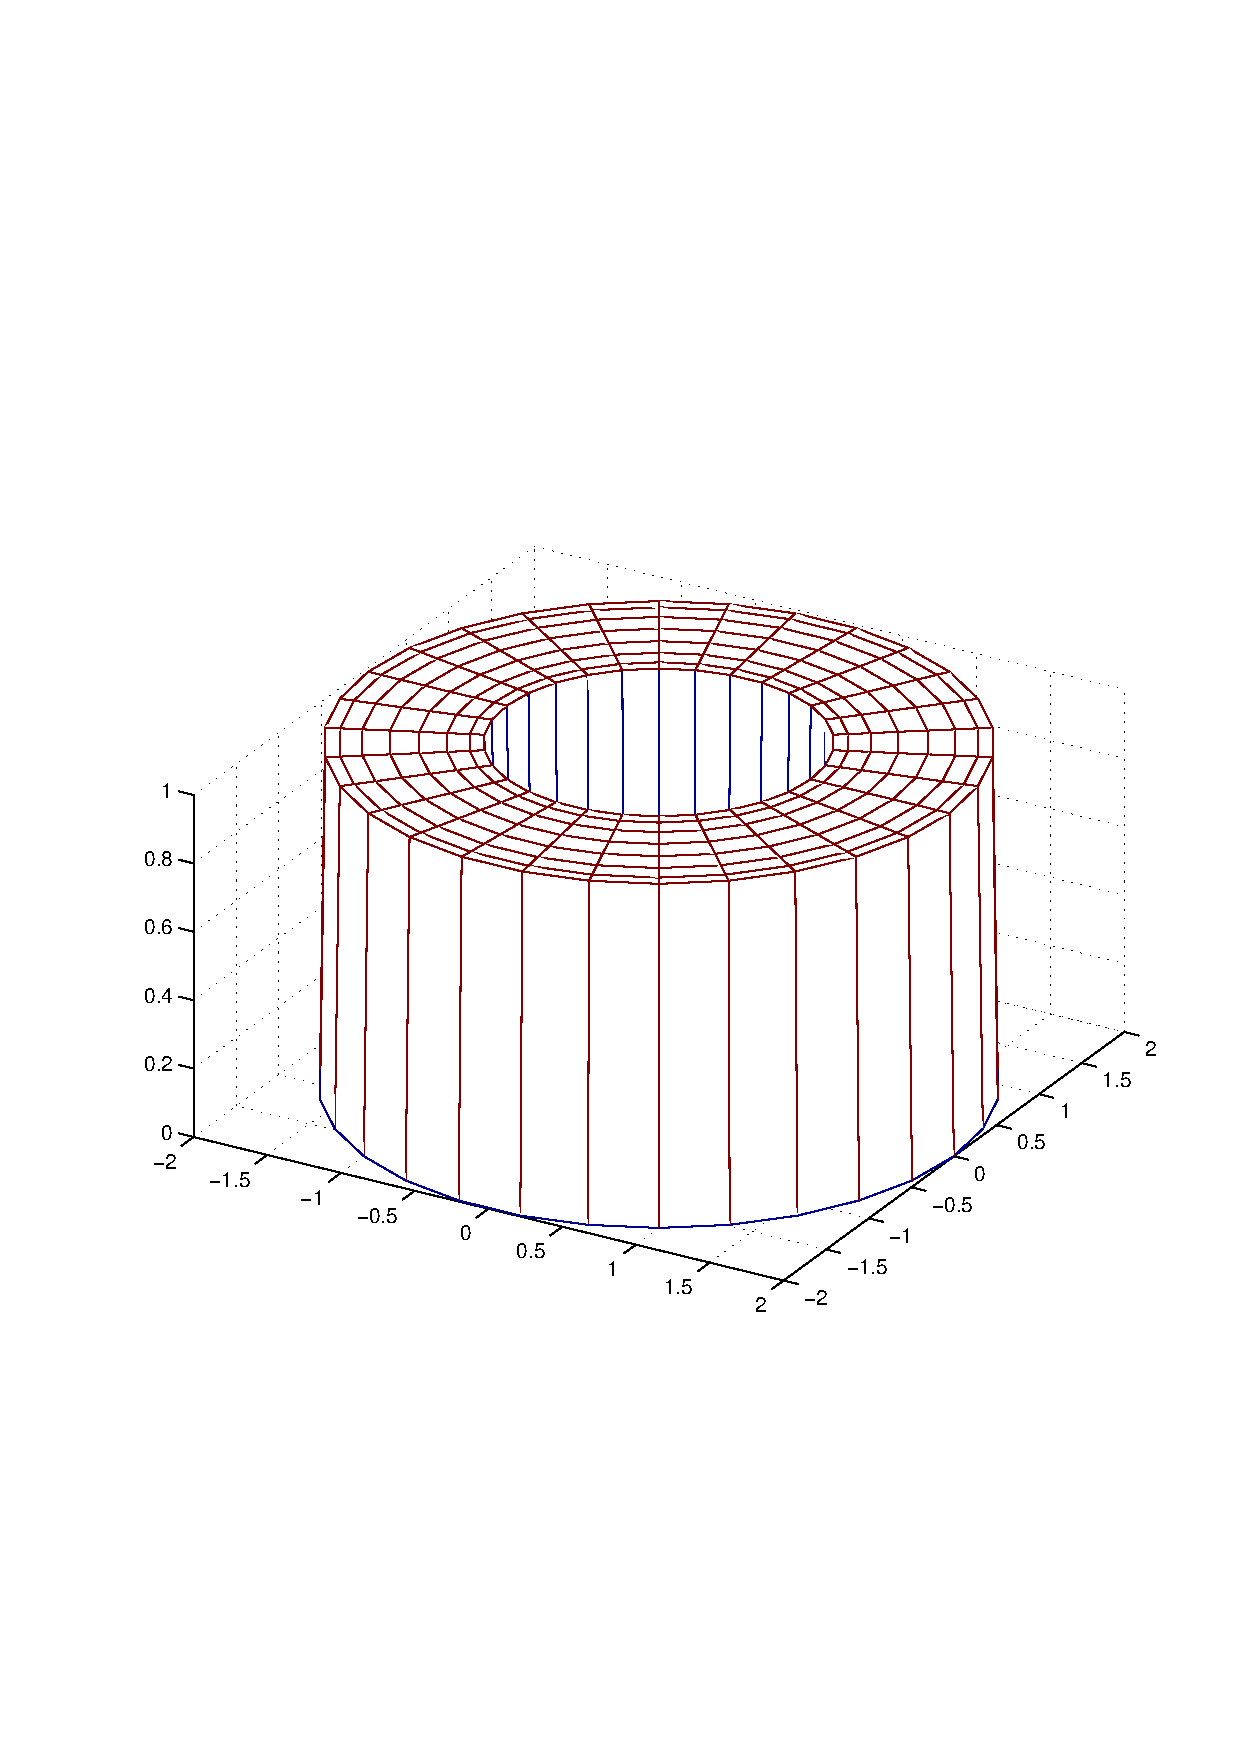
\includegraphics[width=0.55\linewidth]{figures/ringpotential.pdf}
 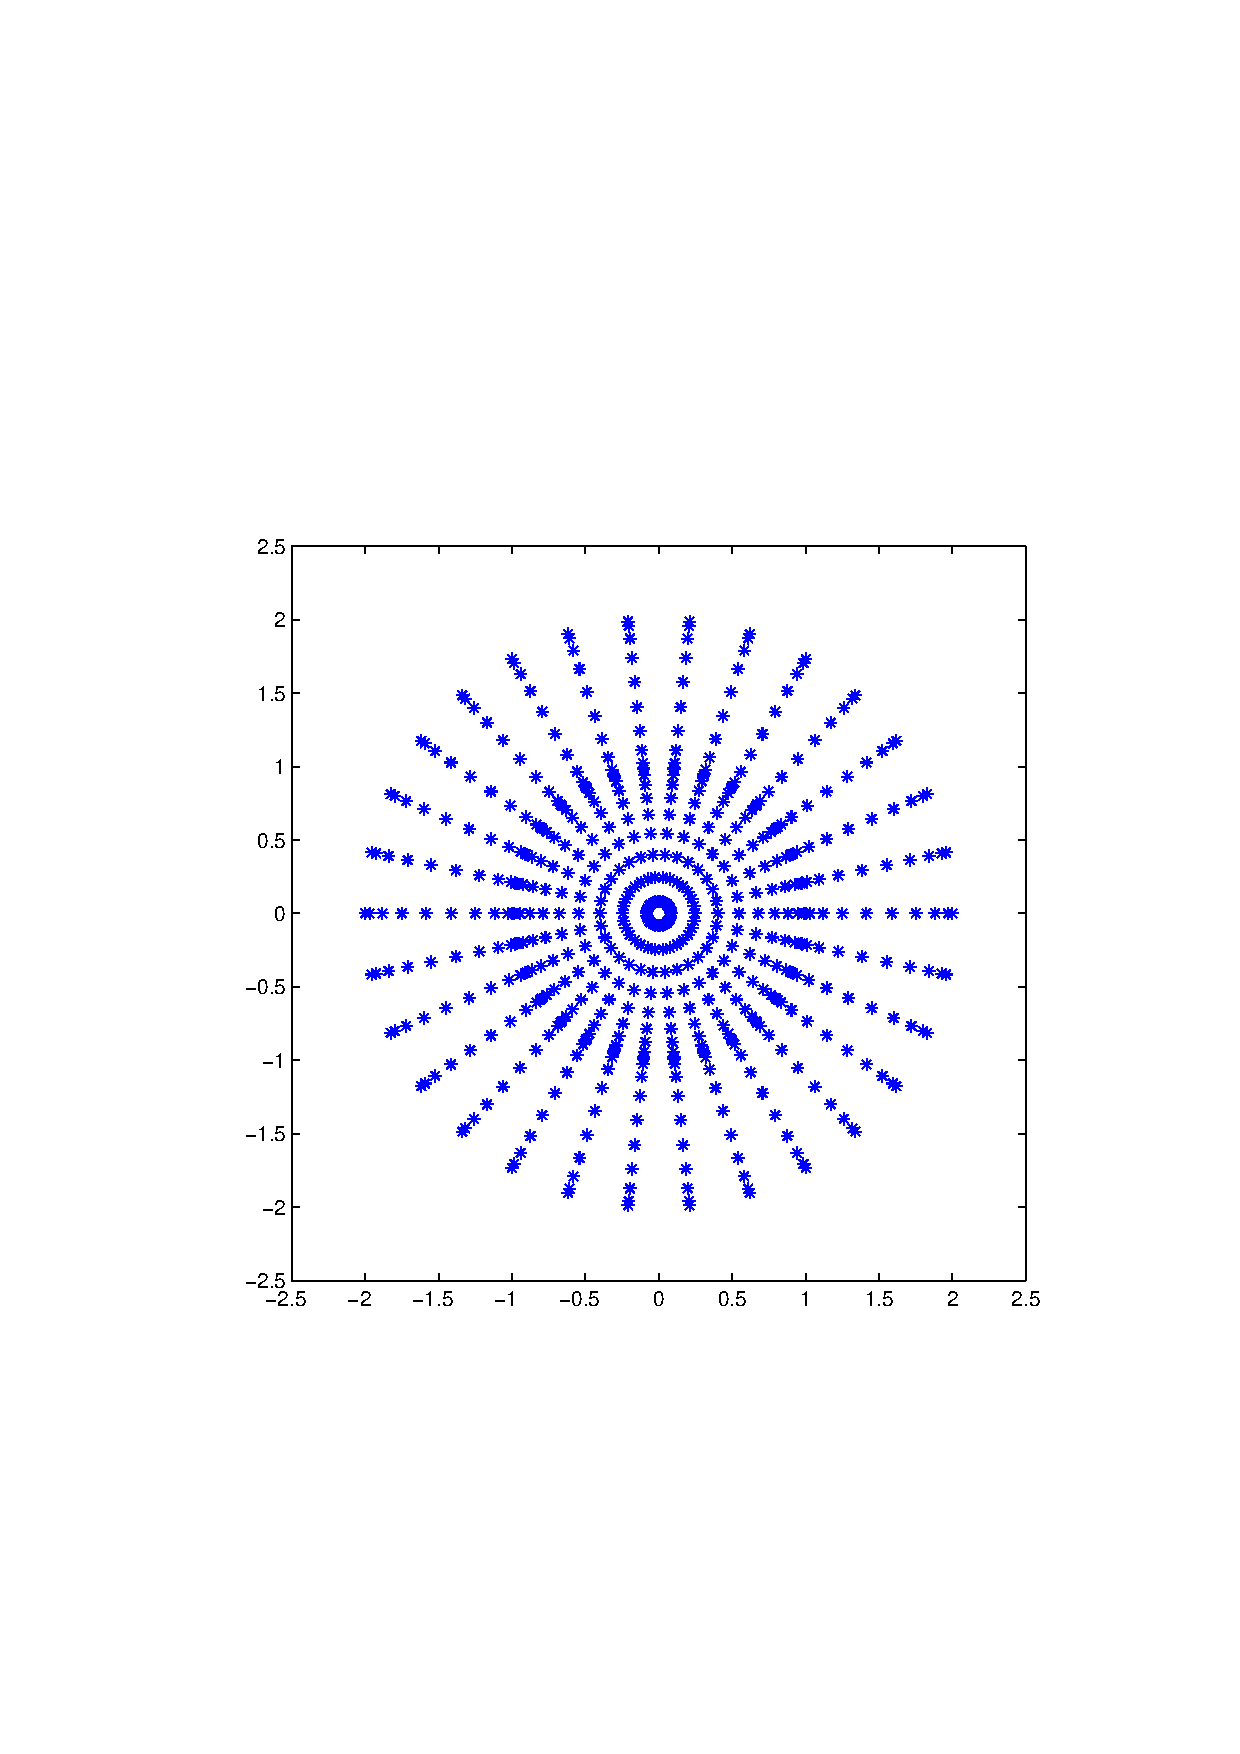
\includegraphics[width=0.45\linewidth]{figures/ringpotentialmesh.pdf} \\ 
 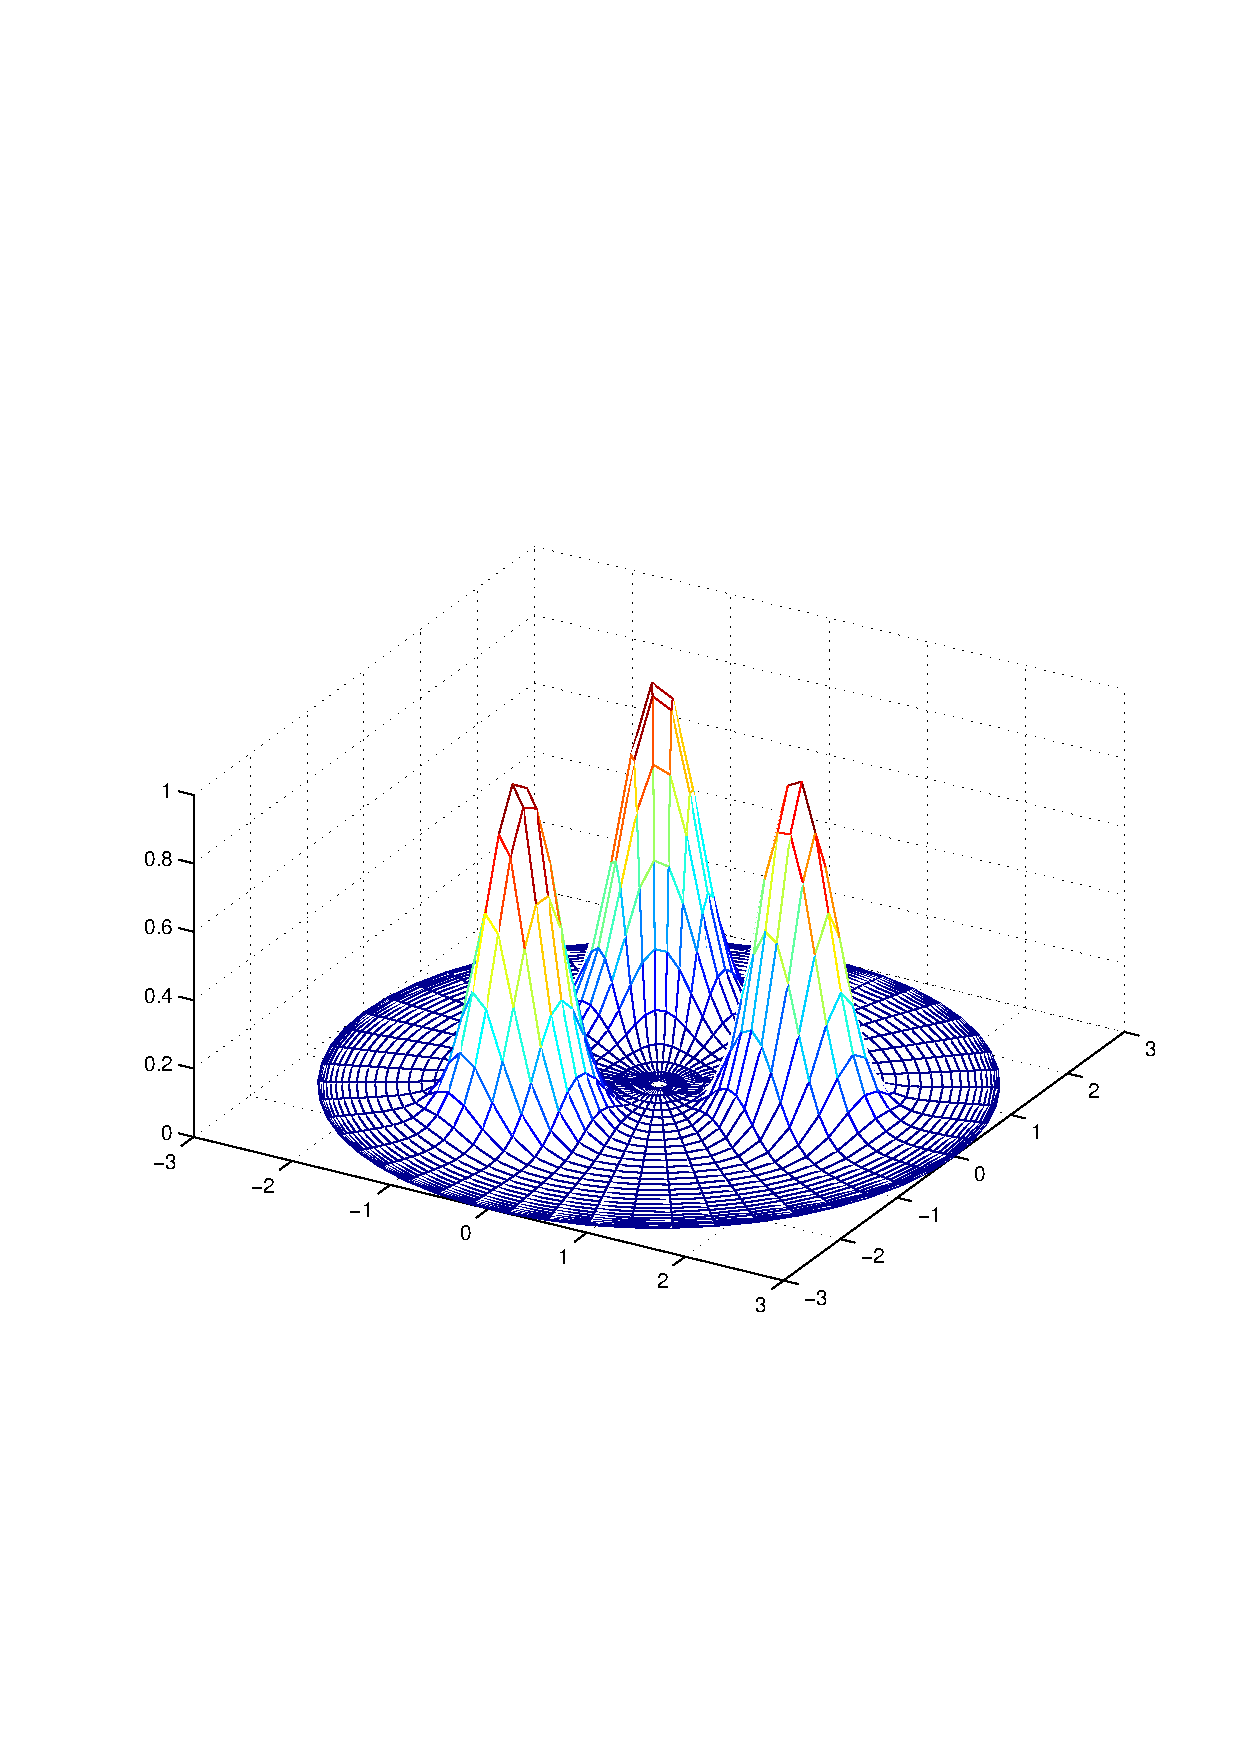
\includegraphics[width=0.55\linewidth]{figures/threebumppotential.pdf}
 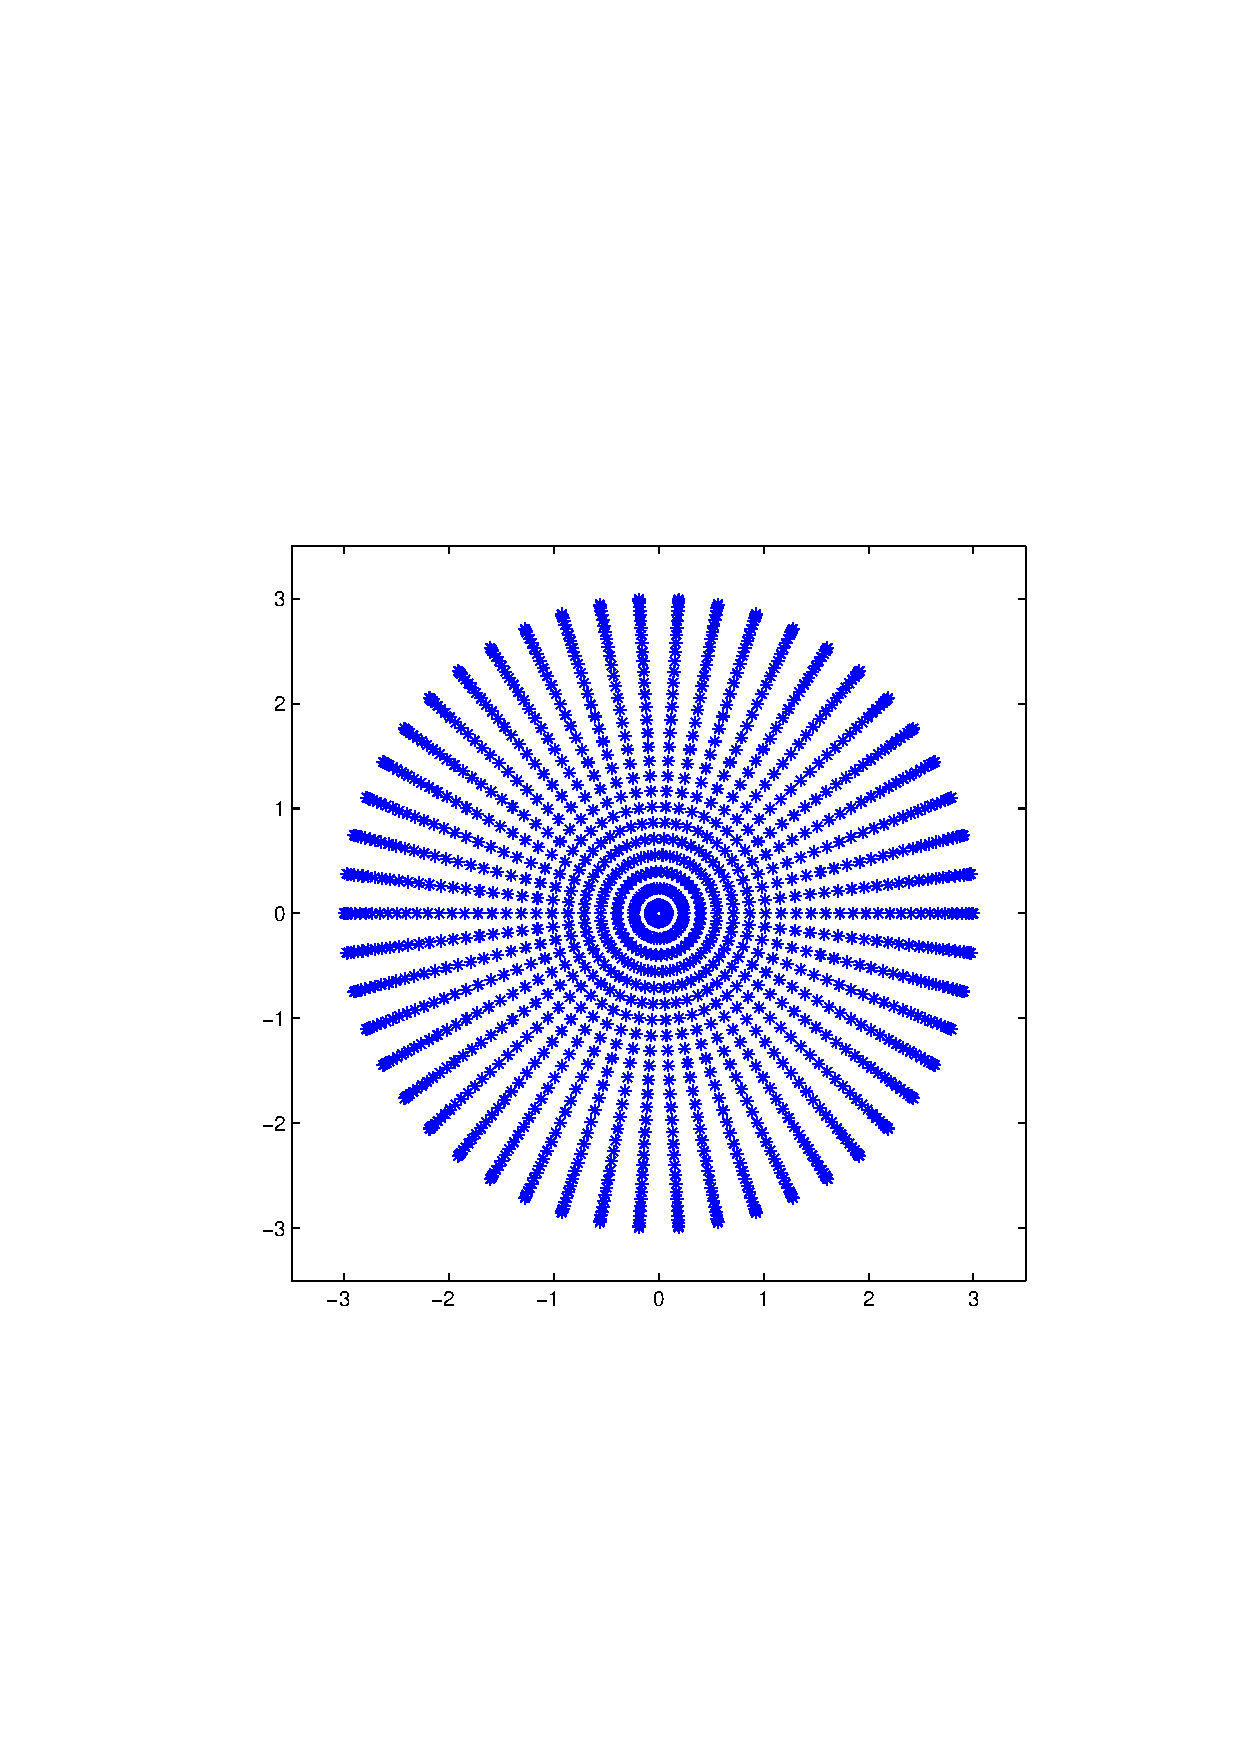
\includegraphics[width=0.45\linewidth]{figures/threebumppotentialmesh.pdf}
 \caption{Top Left: An axisymmetric, piecewise constant potential
                equal to 1 on $1 < r < 2$ and zero elsewhere.
          Top Right: The regions where the potential is constant
                 must be meshed separately.
          Bottom Left: A potential consisting of three bumps. Most
                 of the volume of the potential is contained in
                 $B(0,3)$.
          Bottom Right: Since the potential function is continuous
                 everywhere, the disc $B(0,3)$ can be meshed without
                 splitting it into a central disk and annular regions.}
\end{figure}


\part{Scattering}

\section{Solving the scattering problem}

To solve~(\ref{eqtn-scattprob}), this code uses a
spectral collocation approach. This means we approximate the
values of the scattered wave on a Chebyshev-type mesh.
Different
boundary conditions correspond to different ways of
approximating the outgoing boundary condition. 
In the code, the discretization of the
PDE in~(\ref{eqtn-scattprob}) with 
each boundary condition corresponds
to its own object:
\begin{align*}
 \text{Dirichlet boundary condition on boundary of
  potential support}\quad\leftrightarrow\quad{\tt dirBC} \\
 \text{PML plus Dirichlet boundary condition at outer edge}
  \quad\leftrightarrow\quad{\tt pmlBC} \\
 \text{DtN map boundary condition on boundary of potential
  support}\quad\leftrightarrow\quad{\tt DtNBC}
\end{align*}
These three objects share many properties and methods 
(e.g. for defining discretizations, methods for plotting, etc.), 
so they are children of parent object {\tt scattResComp2d}.

Before describing these objects, there are two more things
to address.
First, since the boundary conditions
will be imposed at a certain radius, polar coordinates
are the most convenient way to represent the scattering
problem~(\ref{eqtn-scattprob}). In particular, it will
be useful to have at hand the Laplacian in polar coordinates:
\begin{equation}\label{eqtn-polarlaplacian}
 \Delta = \frac{\partial^2}{\partial r^2} +
          \frac{1}{r} \frac{\partial}{\partial r} +
          \frac{1}{r^2} \frac{\partial^2}{\partial\theta^2}.
\end{equation}
Second, in all cases the discretization of~(\ref{eqtn-scattprob})
will gives us a matrix equation
\begin{equation}\label{eqtn-defT}
 T(k) \widehat{\scatt} = -\widehat{V\inc}
\end{equation}
where the hat indicates evaluation on the user-specified mesh.
The general form of $T(k)$ is $A - k^2 B + C(k)$, where
$A - k^2 B$ encapsulates the PDE and linear parts of
boundary conditions, and $C(k)$ holds the nonlinear parts of
the boundary conditions (e.g. the DtN map). Therefore each
of the child objects will have a method called {\tt T}.

\section{Using {\tt scattResComp2d}}
\label{sec-scattResComp2d}

The {\tt scattResComp2d} object does the heavy lifting of
bookkeeping, discretizing, and plotting, as well as
having a few other conveniences.

Creating an instance is simple: 
\begin{verbatim}
 >> s = scattResComp2d(Nt,Nrs,Rs);
\end{verbatim}
where
\begin{itemize}
 \item {\tt Nt} is the number of mesh points in the $\theta$
                 direction ({\bf must be even} because of the way
                 the Laplacian is constructed--if you pass an odd
                 {\tt Nt}, it will be increased by one)
 \item {\tt Nrs} is a vector holding the number of mesh points in
                 the radial direction on each concentric subregion
                 (see Sections~\ref{sec-mesh} and~\ref{sec-potential})
 \item {\tt Rs} is a vector holding the outer radius of each
                 subregion.
\end{itemize}
What follows is a description of all properties and methods, grouped
by usage.

\subsection{Easy indexing}
\label{sec-scattResComp2d-indexing}

\begin{description}
 \item[Properties]
   \begin{itemize}
    \item[] % so bullet starts on next line
    \item {\tt Nr} is the total number of mesh points in the 
                 radial direction (sum over {\tt Nrs})
    \item {\tt BCrows} is the vector of row indices where the boundary
                 conditions will be placed
    \item {\tt valRows} is the vector of row indices in each block row
                 where continuity of the scattered wave 
                 across subregions is enforced
    \item {\tt derRows} same as {\tt valRows}, but for enforcing
                 differentiability
    \item {\tt ICBCrows} is the (ordered) vector of row indices where
                 continuity, differentiability, and boundary
                 conditions are enforced
   \end{itemize}
\end{description}

\subsection{Easy mesh representations}
\label{sec-scattResComp2d-mesh}

\begin{description}
 \item[Properties]
   \begin{itemize}  
    \item[] % so bullet starts on next line
    \item {\tt r} is the vector of mesh points in the radial direction
    \item {\tt theta} is the vector of mesh points in the theta direction,
          starting from 0 and not including $2\pi$.
    \item {\tt rr,tt} are matrices of mesh point locations in 
          polar coordinates (from {\tt meshgrid}), used for 3d plotting
    \item {\tt xx,yy} are matrices of mesh point locations in rectangular
          coordinates, same ordering as {\tt rr,tt}
    \item {\tt rs,ts} are vectors of mesh point locations in
          polar coordinates, where {\tt rs} is a stack of copies of the
          vector {\tt r},
          and {\tt ts} has {\tt Nr} copies of {\tt theta(1)} at the top,
          followed by {\tt Nr} copies of {\tt theta(2)}, etc.
    \item {\tt xs,ys} are vectors of mesh point locations in
          rectangular coordinates (same order as {\tt rs,ts})
    \item {\tt zs} is a vector of mesh point locations represented
          in complex coordinates ($z = x + iy$)
   \end{itemize}

 \item[Methods]
   \begin{itemize}
    \item[] % so bullet starts on next line
    \item {\tt valuesVecFromFun(obj,f,coords)} 
          takes a function handle {\tt f} representing a 
          function $f$ on the 
          plane and returns its values on the mesh of $B(0,R)$:
         \begin{description}
          \item[{\tt valuesVecFromFun(obj,f,'rect')}] implies
          $f = f(x,y)$, and returns 
          {\tt f(xs,ys)}, 
          \item[{\tt valuesVecFromFun(obj,f,'polar')}] implies
          $f = f(r,\theta)$ and returns
          {\tt f(rs,ts)}, and
          \item[{\tt valuesVecFromFun(obj,f,'complex')}] implies
          $f = f(z)$ and returns
          {\tt f(zs)}
         \end{description}
    \item {\tt valuesVecFromFunCellArray(obj,fs,coords)} is same
          as {\tt valuesVecFromFun} except {\tt fs} is
          a cell array of functions which represent a piecewise
          continuous function on $B(0,R)$ by continuous functions
          defined for each subregion separately
    \item {\tt plotValuesVec(obj,valuesVec,titlestr,part)}
          makes a 3d plot of the specified part 
          (usually real, imag, or abs)
          of a function given its 
          valuesVec representation, and uses {\tt titlestr} 
          as the title of the
          figure ({\tt part} defaults to {\tt @real} 
          if {\tt []} is passed)
    \item {\tt plotFun(obj,f,titlestr,part,coords)} makes
          3d plot of the specified part (usually real, imag,
          or abs) of the function f
          ({\tt part} defaults to {\tt @real} if {\tt []} is passed.
   \end{itemize}
\end{description}

\subsection{Fourier representations and converting}
\label{sec-scattResComp2d-fourier}

\begin{description}
 \item[Properties]
   \begin{itemize}
    \item[] % so bullet starts on next line
    \item {\tt Ns} is the vector of indices of Fourier series terms that
                 would be computed with the discrete Fourier transform
                 ({\tt -Nt/2 + 1:Nt/2})
    \item {\tt U} is the matrix that maps Fourier coefficients 
                  (with indices {\tt Ns}) to function values on
                  {\tt theta}
    \item {\tt Uinv} is the inverse of {\tt U}, mapping function values
                  to Fourier coefficients
   \end{itemize}

 \item[Methods]
   \begin{itemize}
    \item[] % so bullet starts on next line
    \item {\tt fourierVecFromValuesVec(obj,valuesVec)} 
          transforms a valuesVec into a stack of Fourier
          coefficents with indices {\tt Ns}, each evaluated
          on the radial mesh {\tt r}
    \item {\tt valuesVecFromFourierVec(obj,fourierVec)}
          does the opposite and allows for more or
          fewer Fourier coefficients
    \item {\tt fourierVecFromFun(obj,f,coords)} finds the valuesVec
          for {\tt f} and transforms it to a fourierVec
    \item {\tt fourierVecFromFunCellArray(obj,fs,coords)}
          does what {\tt valuesVecFromFunCellArray} does then
          transforms to a fourierVec
    \item {\tt plotFourierVec(obj,fourierVec,titlestr,part)}
          turns a fourierVec into a valuesVec and plots using
          {\tt plotValuesVec}
    \item {\tt chebVecFromFourierVec(obj,fourierVec)} takes each
          $f_n(\hat{r})$ (where {\tt fourierVec} is a stack of these),
          applies {\tt radialVals2chebCoeffs} (see below)
          and returns the stack of these results
    \item {\tt fourierVecFromChebVec(obj,chebVec)} does the opposite,
          applying {\tt chebCoeffs2radialVals}          
    \item {\tt radialVals2chebCoeffs(obj,v,parity)} takes the values
          {\tt v} of an even or odd function evaluated on the radial mesh
          {\tt r} ({\tt parity} is {\tt 'even'} or {\tt 'odd'}), splits
          into $v_1$, $v_2$, ... according to piecewise radial mesh sizes,
          finds the Chebyshev coefficients $c_m$ of each $v_m$
          (more detail below), and returns the stack of $c_m$'s
    \item {\tt chebCoeffs2radialVals(obj,c,parity)} reverses the process
    \item {\tt halfChebVals2chebCoeffs(v,parity)} takes a vector {\tt v}
          of values of even or odd function $f$ ({\tt parity} is
          {\tt 'even'} or {\tt 'odd'}) on a half Chebyshev mesh of $[0,1]$
          and as many Chebyshev coefficients of $f$ as there are
          values in {\tt v}
    \item {\tt chebCoeffs2halfChebVals(c,parity)} reverses the process
    \item {\tt fullChebVals2chebCoeffs(v)} takes a vector {\tt v} of
          values of a function $f$ on a Chebyshev mesh of $[0,1]$ and
          returns as many Chebyshev coefficients as there are values
    \item {\tt chebCoeffs2fullChebVals(c)} reverses the process
   \end{itemize}
\end{description}

\subsection{Chebyshev representations and converting}
\label{sec-scattResComp2d-chebyshev}

\begin{description}
 \item[Properties]
   \begin{itemize}
    \item[] % so bullet starts on next line
    \item {\tt Winv\_even} is a matrix such that {\tt Winv\_even*c}
          equals {\tt chebCoeffs2radialVals(obj,c,'even')} (see below)
    \item {\tt Winv\_odd} is a matrix such that {\tt Winv\_odd*c}
          equals {\tt chebCoeffs2radialVals(obj,c,'odd')} (see below)
   \end{itemize}
 \item[Methods]
   \begin{itemize}
    \item[] % so bullet starts on next line
    \item {\tt chebVecFromFourierVec(obj,fourierVec)} takes each
          $f_n(\hat{r})$ (where {\tt fourierVec} is a stack of these),
          applies {\tt radialVals2chebCoeffs} (see below)
          and returns the stack of these results
    \item {\tt fourierVecFromChebVec(obj,chebVec)} does the opposite,
          applying {\tt chebCoeffs2radialVals}          
    \item {\tt chebVecFromValuesVec(obj,valuesVec)} converts the stack
          of function values to a stack of Fourier coefficient values to
          a stack of Chebyshev coefficients for those piecewise-defined
          Fourier coefficient functions
    \item {\tt valuesVecFromChebVec(obj,chebVec)} does the opposite
    \item {\tt radialVals2chebCoeffs(obj,v,parity)} takes the values
          {\tt v} of an even or odd function evaluated on the radial mesh
          {\tt r} ({\tt parity} is {\tt 'even'} or {\tt 'odd'}), splits
          into $v_1$, $v_2$, ... according to piecewise radial mesh sizes,
          finds the Chebyshev coefficients $c_m$ of each $v_m$
          (more detail below), and returns the stack of $c_m$'s
    \item {\tt chebCoeffs2radialVals(obj,c,parity)} reverses the process
    \item {\tt halfChebVals2chebCoeffs(v,parity)} takes a vector {\tt v}
          of values of even or odd function $f$ ({\tt parity} is
          {\tt 'even'} or {\tt 'odd'}) on a half Chebyshev mesh of $[0,1]$
          and as many coefficients of the expansion of $f$ in even or odd
          Chebyshev polynomials as there are values in {\tt v} (see
          Section~\ref{sec-cheb_basis})
    \item {\tt chebCoeffs2halfChebVals(c,parity)} reverses the process
    \item {\tt fullChebVals2chebCoeffs(v)} takes a vector {\tt v} of
          values of a function $f$ on a Chebyshev mesh of $[0,1]$ and
          returns as many Chebyshev coefficients as there are values
    \item {\tt chebCoeffs2fullChebVals(c)} reverses the process
   \end{itemize}
\end{description}

\subsection{Creating discretized scattering problem}
\label{sec-scattResComp2d-create}

\begin{description}
 \item[Properties]
   \begin{itemize}
    \item[] % so bullet starts on next line
    \item {\tt Dr} is the matrix that maps $f({\tt rs,ts})$ to
          $\frac{\partial f}{\partial r}({\tt rs,ts})$
    \item {\tt Drr} is the matrix that maps $f({\tt rs,ts})$ to
          $\frac{\partial^2 f}{\partial r^2}({\tt rs,ts})$
    \item {\tt Dtt} is the matrix that maps $f({\tt theta})$ to
          $\frac{\partial^2 f}{\partial\theta^2}({\tt theta})$
          (see Section~\ref{sec-laplacian} for how this relates to discretization
          of last term in Laplacian)
    \item {\tt Drs} is not interesting right now
    \item {\tt Dr\_I}, {\tt Dr\_J}, {\tt Drr\_I}, {\tt Drr\_J}
          are matrices used to construct {\tt Dr} and {\tt Drr}
          according to 
          \begin{verbatim}
           Dr  = kron(It,Dr_I)  + kron(Jt,Dr_J)
           Drr = kron(It,Drr_I) + kron(Jt,Drr_J)
          \end{verbatim}
          (see Section~\ref{sec-piecewise} for derivation of
          {\tt Dr\_I, Dr\_J, Drr\_I} and {\tt Drr\_J})
    \item {\tt It}, {\tt Jt} are {\tt Nt} $\times$ {\tt Nt}
          matrices equaling the identity and 
          $\begin{bmatrix} 0 & I_{half} \\ I_{half} & 0\end{bmatrix}$,
          respectively, where $I_{half}$ is the {\tt Nt/2} identity
          ({\bf this is why {\tt Nt} should be even})
   \end{itemize}

 \item[Methods]
   \begin{itemize}
    \item[] % so bullet starts on next line
    \item {\tt enforceDE} is called only by the child objects
          corresponding to boundary condition choice, and constructs
          the matrices $A$ and $B$ such that $A-k^2B$ is the discretization
          of $-\Delta + V - k^2 I$
    \item {\tt enforceIC, enforceBlockIC}
          replaces the {\tt valRows} and {\tt derRows} of $A$ with
          equations enforcing continuity and differentiability 
          at subregion interfaces and zeros the same rows of $B$
    \item {\tt RHSfromFun(obj,incfun)} will only be called
          after a {\tt dirBC}, {\tt pmlBC} or {\tt DtNBC}
          instance is created, and returns
          the valuesVec for $-V\inc$ 
          (the Right Hand Side of~(\ref{eqtn-scattprob}))
          but with the boundary and
          interface condition rows set to zero--note that 
          {\tt incfun} must be in the same
          coordinates which are specified by {\tt coords}
          when the {\tt *BC} instance is created.
          {\bf Alternatively, the user can pass a wave number $k$
          in place of {\tt incfun}
          and the default {\tt incfun = @(x,y) exp(1i*k*x)} will be used.}
    \item {\tt solve(obj,k,incfun)} will only be called after
          a {\tt dirBC}, {\tt pmlBC} or {\tt DtNBC} instance
          is created and returns the values of the approximate scattered
          wave on the user's mesh of $B(0,R)$--the last argument should
          be omitted to use the default $\inc$. For testing purposes,
          if the user passes a vector for {\tt incfun} the
          vector {\tt T(k)\textbackslash incfun} will be returned.
   \end{itemize}
\end{description}

\subsection{Bessel functions and resonance processing}
\label{sec-scattResComp2d-bessel}

\begin{description}
 \item[Static methods]
   \begin{itemize}
    \item[] % so bullet starts on next line
    \item {\tt sort\_eigs} sorts a vector of eigenvalues from 
          left to right in the complex plane and applies same
          ordering to eigenvectors
    \item {\tt get\_closest(p,n,p0)} takes a vector {\tt p} of
          points and returns a vector of the {\tt n} points
          closest to {\tt p0}
    \item {\tt J, Y} are wrappers for the first and second kind
          Bessel functions built in to \textsc{Matlab}, e.g.
          {\tt J(n,k,x) = besselj(n,k*x)}, and 
          {\tt J(n,k,x)} $= J_n(kx)$
    \item {\tt H} is a wrapper for the first kind Hankel function
          built in to \textsc{Matlab} (first kind corresponds to
          outgoing waves)
    \item {\tt dJ, dY, dH} are derivatives of {\tt J, Y, H} 
          with respect to the third variable, e.g.
          {\tt dJ(n,k,x)} $= k J_n'(kx)$
   \end{itemize}
\end{description}

\subsection{Not important right now}
\label{sec-scattResComp2d-unimportant}

\begin{description}
 \item[Properties not worth describing right now]
   \begin{itemize}
    \item[] % so bullet starts on next line
    \item {\tt valRows\_cc}, {\tt derRows\_cc}, 
          {\tt ArowChange}, {\tt BrowChange}, 
          {\tt rowPlacement}
   \end{itemize}

 \item[Methods not worth describing right now]
   \begin{itemize}
    \item[] % so bullet starts on next line
    \item {\tt RHSfromFun\_cc}, {\tt dLogTz},
          {\tt plotRayValuesVec}
   \end{itemize}
\end{description}

\section{Solving the scattering problem with {\tt dirBC}}
\label{sec-dirBC}

This object allows the user to solve the
scattering~(\ref{eqtn-scattprob}) and
resonance~(\ref{eqtn-resprob}) problems with Dirichlet boundary
conditions.

\subsection{The boundary condition}
\label{sec-dirBC-BC}

A Dirichlet boundary condition (rather than the outgoing
condition) in~(\ref{eqtn-scattprob})
means enforcing that $\scatt(R) = 0$, giving the following
boundary value problem:
\begin{equation}\label{eqtn-dirprob}
\begin{aligned}
 \left(-\Delta + V - k^2\right)\scatt &= -V\inc
 \qquad
 \text{on }B(0,R), \\
 \scatt(R) &= 0.
\end{aligned} 
\end{equation}
The solution to~(\ref{eqtn-dirprob}) is a good approximation to
the solution to~(\ref{eqtn-scattprob}) in case the potential has 
very thick, high walls that very quickly attenuate the scattered wave.

Discretizing~(\ref{eqtn-dirprob}) amounts to taking the matrices $\dirA$
and $\dirB$ that come from discretizing the PDE and
replacing the boundary condition rows of $\dirA$ and $\dirB$ with
rows of the identity and zeros, respectively. 
Then if $\dirT(k) = \dirA - k^2 \dirB$, 
$\dirT(k)\widehat{\scatt} = -\widehat{V\inc}$,
where the hat indicates values on the mesh of $B(0,R)$.
The object
{\tt dirBC} encapsulates the discretization of~(\ref{eqtn-dirprob}).

\subsection{Creating an instance}
\label{sec-dirBC-create}

Create an instance with
\begin{verbatim}
 >> dir = dirBC(Nt,Nrs,Vs,coords,Rs);
\end{verbatim}
where the potential $V$ is specified with cell array {\tt Vs}
(see above) and {\tt coords} equals 'rect', 'polar', or 'complex'
depending on whether $V = V(x,y)$, $V = V(r,\theta)$, or
$V = V(z)$.

\subsection{Properties and methods}
\label{sec-dirBC-properties}

Here are properties and methods, in addition to those
available through
parent object {\tt scattResComp2d}:
\begin{description}
 \item[Properties]
   \begin{itemize}
    \item[]
    \item {\tt Vs, coords} are as described above
    \item {\tt A, B} are the matrices $\dirA$ and $\dirB$ described above;
          the values of the scattered wave on the mesh solve
          $\dirT(k)\widehat{\scatt} = -\widehat{V\inc}$
%%%%%%%%%%%%%%%%%%%%%%%%%%%%%%%%%%%%%%%%%%%%%%%%%%%%%%                        
% Lr probably doesn't need to be a property                                    
%%%%%%%%%%%%%%%%%%%%%%%%%%%%%%%%%%%%%%%%%%%%%%%%%%%%%%%%%%%%                    
    \item {\tt Lr} is the discretization of the radial part of the
          Laplacian, $\frac{\partial^2}{\partial r^2} +     
          \frac{1}{r}\frac{\partial}{\partial r}$, no boundary
          or interface conditions applied
    \item {\tt evecs,evals} are the eigenvalues $E$ and their
          eigenvalues, computed when {\tt eig\_comp()} is called
    \item {\tt A\_orig}, {\tt B\_orig}, {\tt A\_cc}, {\tt B\_cc},
          aren't important right now and
          not all of them need to be properties, probably
   \end{itemize}
 \item[Methods]
   \begin{itemize}
    \item[]
    \item {\tt enforceBC(obj)} adjusts boundary condition rows of 
          $\dirA$ and $\dirB$
          as described above
    \item {\tt T(obj,k)} returns the matrix $\dirT(k)$
%%%%%%%%%%%%%%%%%%%%%%%%%%%%%%%%%%%%%%%%%%%%%%%%%%%%%%%%%%%     
% kinda outdated
%%%%%%%%%%%%%%%%%%%%%%%%%%%%%%%%%%%%%%%%%%%%%%%%%%%%%%%%%%%%                 
    \item {\tt eig\_comp(obj)} computes the eigenvalues of the pencil
          $(\dirA,\dirB)$ to find resonances
   \end{itemize}
\end{description}

\subsection{Solving the scattering problem}
\label{sec-dirBC-solvescattprob}

The boundary value problem~(\ref{eqtn-dirprob})
is specified completely with the following three things:
\begin{itemize}
 \item a potential function $V$ (supported in some $B(0,R)$),
 \item wave number $k$, and
 \item incident wave $\inc$ satisfying $-\Delta\inc = k^2 \inc$.
\end{itemize}
Analogously, 
the discretization of~(\ref{eqtn-dirprob}) is specified completely
with 
\begin{itemize}
 \item a {\tt dirBC} instance, 
 \item a wave number {\tt k}, and 
 \item an incident wave {\tt incfun}. 
\end{itemize}
Given {\tt k} the default incident wave
is {\tt incfun = @(x,y) exp(1i*k*x)}.

Supposing a {\tt dirBC} instance (let's call it {\tt dir}) 
has already been created and the user
wants to use the default incident wave {\tt incfun = @(x,y) exp(1i*k*x)},
solving the scattering problem with frequency parameter
{\tt k} can be done in one line:
\begin{verbatim}
 >> scattValuesVec = dir.solve(k);
\end{verbatim}

If the user wants to use a different incident wave (satisfying
$-\Delta\inc = k^2\inc$), solving is still a one-liner:
\begin{verbatim}
 >> scattValuesVec = dir.solve(k,incfun);
\end{verbatim}

Here is 
a full example using the default $\inc = e^{ikx}$ and a piece-wise
constant ring potential equal to 0 on $0 \le r \le 1$ and
equal to 1 on $1 < r \le 2$:
\begin{verbatim}
 >> Vs = {@(r,t) 0*r; @(r,t) 1 + 0*r};
 >> coords = 'polar';
 >> Nt = 20;
 >> Nrs = [30, 30];
 >> Rs = [1,2];
 >> dir = dirBC(Nt,Nrs,Vs,coords,Rs);
 >> k = 2;
 >> scattValuesVec = dir.solve(k);
\end{verbatim}

\section{Solving the scattering problem with {\tt pmlBC}}
\label{sec-pmlBC}

\subsection{The PML and the boundary condition}
\label{sec-pmlBC-BC}

The PML we use consists of an increasing, differentiable coordinate change
$r \mapsto s = r + i \lambda(r)$ such that $s = r$ on $B(0,R)$.
Usually we say $\lambda(r) = \int_0^r \sigma(t)\,dt$ for some
simple function $\sigma$ equal to 0 on $B(0,R)$ and
$\sigma(t) = a(t-R)^p$ otherwise.
\begin{figure}[h]
 \centering
 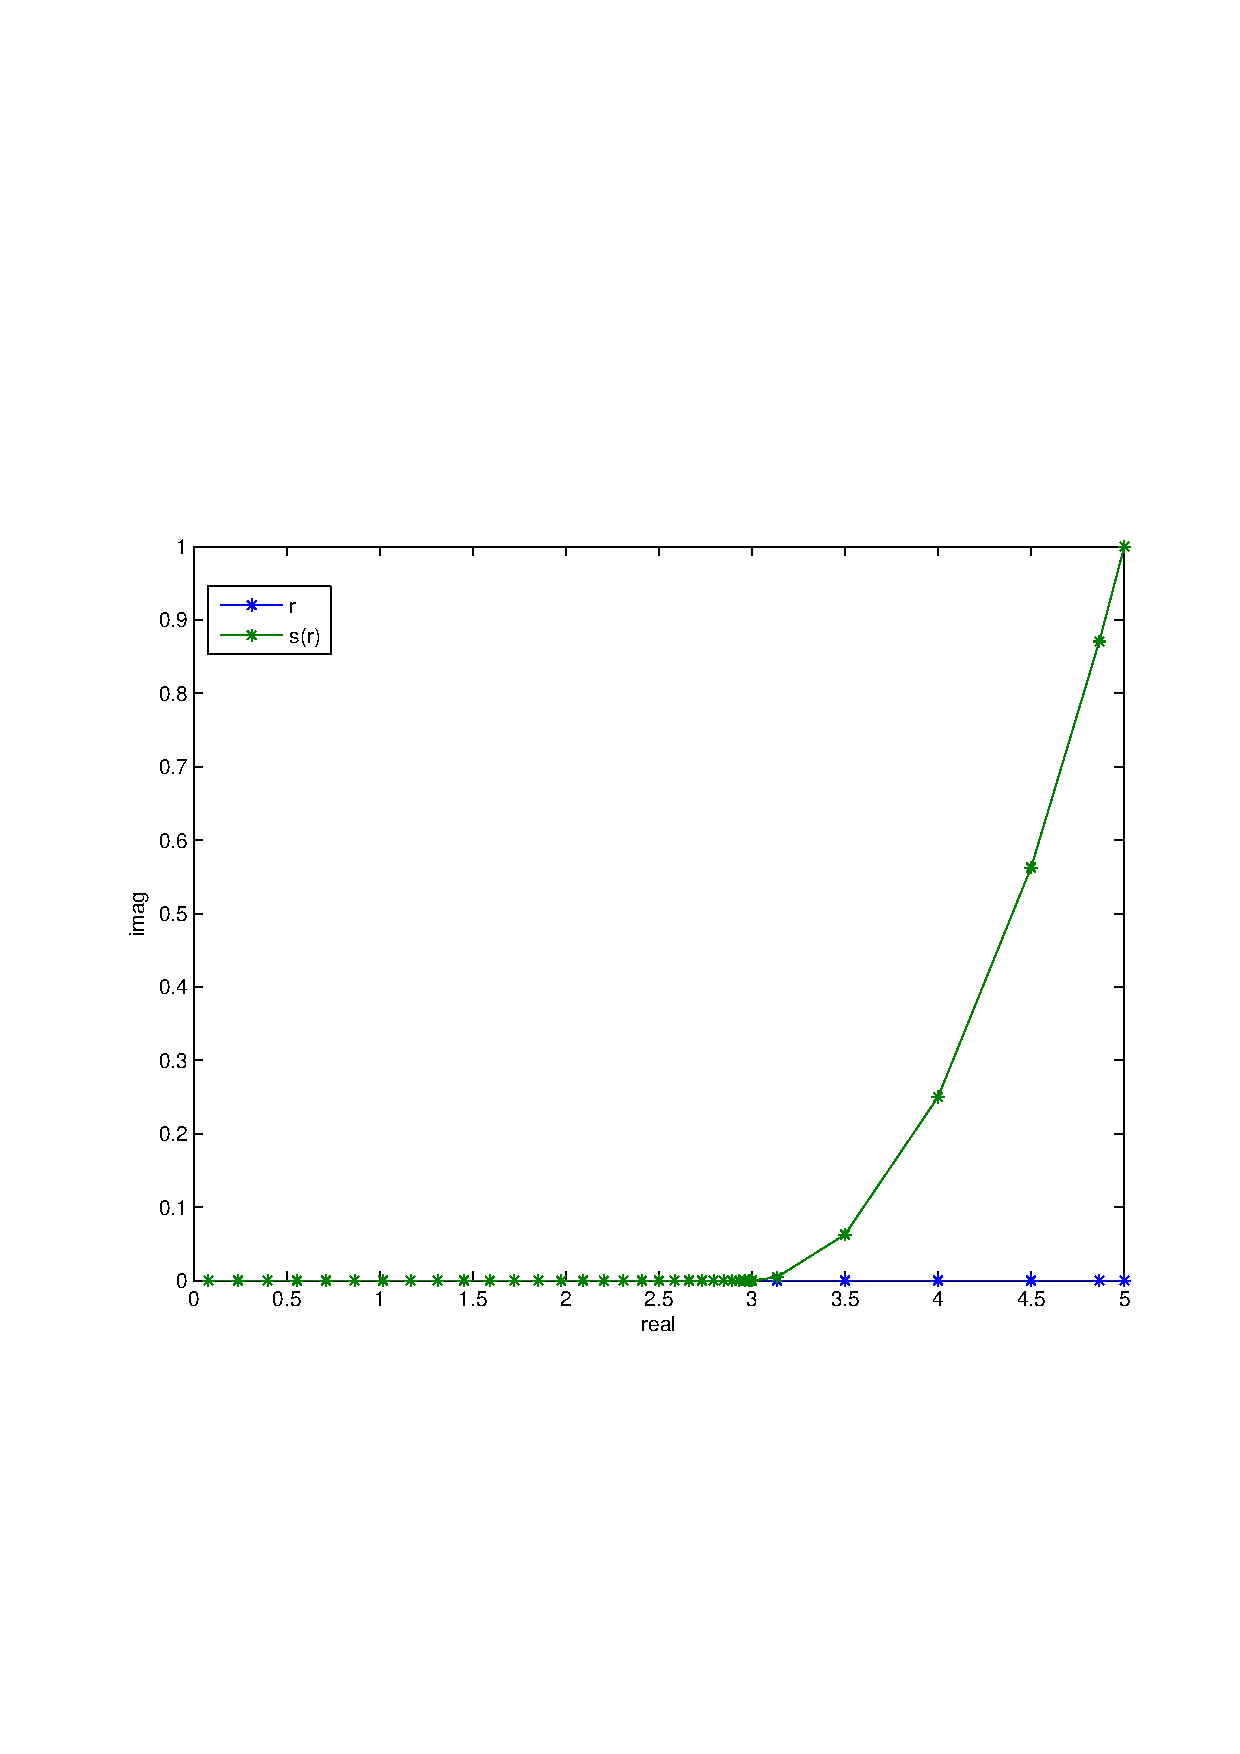
\includegraphics[width=0.6\linewidth]{figures/pml.pdf}
 \caption{PML coordinate function $s$ and mesh points
         {\tt s} and {\tt r} for
	 $\sigma(t) = \chi_{r > 3} \frac{1}{2}(r-3)$.
         The faster the increase, the more mesh points
	 are needed to avoid spurious reflection.
         If the PML is not long
         enough, the scattered wave will not have attenuated
         sufficiently for the Dirichlet boundary condition to
	 pick it out.}
\end{figure}

To solve the scattering problem with a PML is to formally substitute
the new variable $s$ in place of $r$ in~(\ref{eqtn-scattprob})
and use the chain rule to rewrite in terms of $r$ once again
(see Section~\ref{sec-pml} for a little more detail).
The boundary condition is
a Dirichlet boundary condition imposed at some radius
$R_{\text{PML}} > R$ at which the user supposes the scattered wave
has been sufficiently attenuated. Altogether, the scattering problem with
a PML is
\begin{equation}\label{eqtn-pmlscattprob}
\begin{aligned}
(-\Delta_s + V(s(r)) - k^2)\scatt(s(r)) &= -V(s(r))\inc(s(r))
    \qquad \text{on } B(0,R_{\text{PML}}), \\
    \scatt(s(R_{\text{PML}})) &= 0
    \end{aligned}
\end{equation}
where
\begin{equation}\label{eqtn-pmllaplacian}
\begin{aligned}
\Delta_s &= \frac{\partial^2}{\partial s^2} +
\frac{1}{s}\frac{\partial}{\partial s} +
\frac{1}{s^2}\frac{\partial^2}{\partial\theta^2}, \\
				  \frac{\partial}{\partial s}
&= \frac{1}{s'(r)}\frac{\partial}{\partial r}, \\
 \frac{\partial^2}{\partial s^2}
          &= -\frac{s''(r)}{s'(r)^3} \frac{\partial}{\partial r}
+\frac{1}{s'(r)^2} \frac{\partial^2}{\partial r^2}.
\end{aligned}
\end{equation}

The boundary condition is linear, so the discretization
of~(\ref{eqtn-pmlscattprob}) gives a matrix equation
of the form 
$(\pmlA - k^2 \pmlB)\widehat{\scatt}^{(\text{ext})} 
= -\widehat{V\inc}^{(\text{ext})}$
just as in Section~\ref{sec-dirBC-BC},
although here the hat indicates evaluation on the mesh of
$B(0,R_{\text{PML}})$. To make a problem on the mesh of
$B(0,R)$, which makes for more convenient comparisons, we can
take a Schur complement of
\begin{equation}
\underbrace{
\begin{bmatrix}\pmlA_{11} & \pmlA_{12} \\ 
               \pmlA_{12} & \pmlA_{22}\end{bmatrix}}_{\pmlA}
- k^2
\underbrace{
\begin{bmatrix} \pmlB_{11} & 0 \\ 
                         0 & \pmlB_{22}\end{bmatrix}}_{\pmlB}
\underbrace{
 \left[\begin{array}{l}
        \widehat{\scatt} \\
        \widehat{\scatt}^{(\text{PML})}
 \end{array}\right]}_{\widehat{\scatt}^{(\text{ext})}}
 =
 \begin{bmatrix} -\widehat{V\inc} \\ 0 \end{bmatrix}
\end{equation}
to get
\begin{equation}\label{eqtn-pmlschur}
      \left((\pmlA_{11} - k^2 \pmlB_{11}) -
  \pmlA_{12}(\pmlA_{22} - k^2 \pmlB_{22})^{-1}\pmlA_{21}\right)
  \widehat{\scatt} = -\widehat{V\inc}.
\end{equation}
Comparison with~(\ref{eqtn-defT}) shows that in the case of
the PML, we should define $\pmlT(k)$ as the operator
in~(\ref{eqtn-pmlschur}). So they have names, we define
$\pmlT_{\text{full}}(k) = \pmlA - k^2 \pmlB$, and define the
nonlinear part of $\pmlT(k)$ as
$\pmlC(k) = -\pmlA_{12}(\pmlA_{22} - k^2 \pmlB_{22})^{-1} \pmlA_{21}$.
{\bf
It's worth noting that $\pmlC(k)$ contains rational approximations
to the DtN map, and the rational approximations are good for
$k$ values with small, positive real part.}

\subsection{Creating an instance}
\label{sec-pmlBC-create}

Finally, to create an instance of {\tt pmlBC}, do
\begin{verbatim}
 >> pml = pmlBC(Nt,Nrs_in,Nr_out,Vs,coords,Rs_in,R_out,l,dl,d2l);
\end{verbatim}
where {\tt Nrs\_in} and {\tt Rs\_in} equal the previously introduced
{\tt Nrs} and {\tt Rs}, and the new parameters are as follows:
\begin{itemize}
 \item {\tt R\_out} is the outer radius where the PML ends and the
       Dirichlet boundary condition is imposed (called $R_{\text{PML}}$
       above)
 \item {\tt Nr\_out} is the number of mesh points in the radial direction
       for the mesh of [{\tt Rs\_in(end), R\_out}]
 \item {\tt l,dl,d2l} is the function $\lambda(t)$ described above and
       its derivatives
\end{itemize}

\subsection{Properties and methods}
\label{sec-pmlBC-properties}

Since {\tt scattResComp2d} is the parent of {\tt pmlBC},
{\tt pmlBC} inherits all its properties and methods. The rest of the
properties and methods follow.
\begin{description}
 \item[Properties]
   \begin{itemize}
    \item[]
    \item {\tt s} is the transformed radial mesh points on [{\tt 0, R\_out}]
    \item {\tt ss} is the stack of copies of {\tt s}, analogous to {\tt rs}
    \item {\tt Ds, Dss} are the discretizations of
          $\partial/\partial s$ and $\partial^2/\partial s^2$, resp.
    \item {\tt A,B} are the matrices $\pmlA$ and $\pmlB$
    \item {\tt Vs, coords} is a cell array representing the potential, where
          the last entry is always the zero function since $V = 0$
          in the PML region, and the coordinates in which the potential
          functions are given (always {\tt 'rect'}, {\tt 'polar'}, or
          {\tt 'complex'}
    \item {\tt Lr} is the discretization of the radial part of
          $\Delta_s$
    \item {\tt pieces} is a {\tt schurComp} object storing the indices
          for the Schur complement used to create $\pmlT(k)$, etc.
    \item {\tt evecs,evals} are the eigenvalues $E$ and their eigenvectors
          which will be created only after calling {\tt eig\_comp()}x
    \item {\tt A\_orig, B\_orig, A\_cc, B\_cc, ds, d2s} aren't
          important right now and may not stay around
	\end{itemize}
 \item[Methods]
   \begin{itemize}
    \item[]
    \item {\tt enforceBC(obj)} sets the last row of $\pmlA$ and $\pmlB$
	  in the same way as {\tt dirBC.enforceBC()}
    \item {\tt T(obj,k), dT(obj,k)} is the discretization of
	  the function $\pmlT(k)$
	  described above, as well as its derivative with respect to $k$
    \item {\tt Tfull(obj,k)} is the discretization of the
	  function $\pmlT_{\text{full}}(k)$
          described above
    \item {\tt C(obj,k)} returns the matrix $\pmlC(k)$
    \item {\tt RHSfromFun(obj,incfun)} overrides {\tt scattResComp2d.RHSfromFun()}
          to make a right-hand side of the right dimension for $\pmlT(k)$
    \item {\tt RHSfromFun\_full(obj,incfun)} makes a right-hand side of
          the right dimension for $\pmlT_{\text{full}}(k)$
    \item {\tt solve\_full(obj,k,incfun)} works the same way as
          {\tt scattResComp2d.solve()} except returns values on entire
          mesh, including PML region
    \item {\tt eig\_comp(obj)} computes all eigenvalues of the pencil $(\pmlA,\pmlB)$
   \end{itemize}
\end{description}

\subsection{Solving the scattering problem}
\label{sec-pmlBC-solvescattprob}

Much as in Section~\ref{sec-dirBC-solvescattprob}, with a
{\tt pmlBC} instance (call it {\tt pml}) and a choice of $k$,
computing the scattered wave is done with
\begin{verbatim}
 >> scattValuesVec = pml.solve(k);
\end{verbatim}
if the user wants to use the default $\inc$, and
\begin{verbatim}
 >> scattValuesVec = pml.solve(k,incfun);
\end{verbatim}
to specify their own. Similarly, to get the values
of the scattered wave on $B(0,R_{\text{PML}})$, do
\begin{verbatim}
 >> scattValuesVec_ext = pml.solve_full(k);
\end{verbatim}

Here is a full example, complete with the creation of a {\tt pmlBC}
instance. The potential is axisymmetric and piecewise constant, 
equal to 40 on $1.5 \le r \le 2.5$ and zero elsewhere.
\begin{verbatim}
 >> Nt = 30;
 >> Nrs_in = [20,20];
 >> Nr_out = 40;
 >> Vs = {@(r,t) 0*r, @(r,t) 0*r + 40, @(r,t) 0*r};
 >> coords = 'polar';
 >> Rs_in = [1.5,2.5];
 >> R_out = 8;
 >> a = 0.4;
 >> l = @(t) a*(t-R_out).^3;
 >> dl = @(t) a*3*(t-R_out).^2;
 >> d2l = @(t) a*3*2*(t-R_out);
 >> pml = pmlBC(Nt,Nrs_in,Nr_out,Vs,coords,Rs_in,R_out,l,dl,d2l);
 >> k = sqrt(1.5);
 >> scattValuesVec = pml.solve(k);
\end{verbatim}

\section{Solving the scattering problem with {\tt DtNBC}}
\label{sec-DtNBC}

A DtN map boundary condition is an exact boundary condition
for the scattering problem, meaning that an outgoing wave
(and only an outgoing wave) will satisfy this boundary condition
exactly. Therefore, out of the three methods we present here,
we expect this one to produce the most accurate solution
to~(\ref{eqtn-scattprob}).

\subsection{The boundary condition}
\label{sec-DtNBC-BC}

The natural setting for the DtN map is in Fourier space.
Specifically, 
\begin{equation}\label{eqtn-dtnmap}
 \sum_n c_n e^{in\theta} 
 \quad\xmapsto{\text{DtN map}}\quad
 \sum_n f_n(k,R) c_n e^{in\theta},
 \qquad
 f_n(k,R) = k\frac{\left(H_n^{(1)}\right)'(kR)}{H_n^{(1)}(kR)}.
\end{equation}

The set of first- and second-kind Hankel functions 
$\lbrace H_n^{(1)}(kr), H_n^{(2)}(kr) \rbrace_{n=-\infty}^\infty$
form a basis for the solution space of the PDE
in~(\ref{eqtn-scattprob}). 
The first-kind Hankel functions $H_n^{(1)}(kr)$ are a basis for the
space of outgoing waves. 
So, a general solution 
$\sum_n c_n(r) e^{in\theta}$ with
$c_n(r) = a_n H_n^{(1)}(kr) + b_n H_n^{(2)}(kr)$
is an outgoing wave only if all the $b_n$'s are zero.
To guarantee this, we require
\begin{equation}\label{eqtn-dtnbc}
 c_n'(R) = f_n(k,R) c_n(R) \qquad \forall n,
\end{equation}
which is what we mean by the {\bf DtN map boundary condition}.
See Section~\ref{sec-dtn_map} for a derivation.

Now, we can't enforce this for all $n$. The best we can do is
to enforce it for $n = -{\tt Nt}/2 + 1, ..., 0, 1, 2, ... {\tt Nt}/2$,
that is, a number of Fourier coefficients equal to the number of
$\theta$ mesh points and corresponding to lowest frequencies.
To apply the DtN map to the vector
$x = [c_{-{\tt Nt}/2 + 1}({\tt r}), ..., c_{{\tt Nt}/2}({\tt r})]$
of these Fourier coefficients evaluated on the radial
mesh {\tt r}, we have to multiply by the diagonal matrix
$X(k) = \diag\left([f_{-{\tt Nt}/2 + 1}(k,R), ... , f_{{\tt Nt}/2}(k,R)]\right)
\otimes e_{{\tt Nr}} e_{{\tt Nr}}^T$. Therefore, applying
the DtN map to $\widehat{\scatt}$ involves transforming to
the Fourier representation $x$, applying the diagonal operator, and
transforming back. The matrix accomplishing this is
\begin{equation}
 \dtnC(k) = -({\tt U} \otimes I) X(k) ({\tt Uinv} \otimes I),
\end{equation}
with {\tt U, Uinv} as described in Section~\ref{sec-scattResComp2d-fourier}
and full derivation of $\dtnC(k)$ in Section~\ref{sec-dtnC}.
The discretization of~(\ref{eqtn-scattprob}) with DtN map
boundary conditions will then be
\begin{equation}\label{eqtn-Tdtn}
 \left( \dtnA - k^2 \dtnB + \dtnC(k) \right) \widehat{\scatt} = -\widehat{V\inc}.
\end{equation}
Comparison with~(\ref{eqtn-defT}) shows that we should take
$\dtnT(k) = \dtnA - k^2 \dtnB + \dtnC(k)$.

\subsection{Creating an instance}
\label{sec-DtNBC-create}

Same inputs as {\tt dirBC}:
\begin{verbatim}
 >> dtn = DtNBC(Nt,Nrs,Vs,coords,Rs);
\end{verbatim}

\subsection{Properties and methods}
\label{sec-DtNBC-properties}

Inherits properties and methods of parent {\tt scattResComp2d}, and
here's more:
\begin{description}
 \item[Properties]
   \begin{itemize}
    \item[]
    \item {\tt A,B} are the matrices $\dtnA$ and $\dtnB$
    \item {\tt Vs,coords} are the same as for {\tt dirBC}
    \item {\tt Lr} is matrix of radial part of discretization of Laplacian
    \item {\tt A\_orig, B\_orig, A\_cc, B\_cc} not important right now 
   \end{itemize}
 \item[Methods]
   \begin{itemize}
    \item[]
    \item {\tt enforceBC(obj)} sets the boundary condition 
          rows of $\dtnA$ with derivative part of boundary condition
          and zeros those rows of $\dtnB$
    \item {\tt enforceBlockBC(obj,n,X)}
          is called by {\tt enforceBC()}
    \item {\tt enforceBC\_cc(obj)} isn't important right now
    \item {\tt T(obj,k)} returns $\dtnT(k)$ matrix described above
    \item {\tt dT(obj,k), d2T(obj,k)} return the first and second
          derivatives of $\dtnT(k)$ with respect to $k$
    \item {\tt T\_cc(obj,k)} not important right now
    \item {\tt C(obj,k)} returns the matrix $\dtnC(k)$ described above
    \item {\tt C\_cc(obj,k)} not important right now
    \item {\tt dLogTz(obj,z,br), d2LogTz(obj,z,br)} not important right now
   \end{itemize}
 \item[Static Methods]
   \begin{itemize}
    \item[]
    \item {\tt DtNcoeffs(n,k,R)} returns $f_n(k,R)$ as described above
    \item {\tt dDtNcoeffs(n,k,R)} returns first derivative of $f_n$ with
          respect to $k$, evaluated at $k,R$
    \item {\tt d2DtNcoeffs(n,k,R)} returns second derivative with respect
          to $k$, evaluated at $k,R$
   \end{itemize}    
\end{description}

\subsection{Solving the scattering problem}
\label{sec-DtNBC-solvescattprob}

See Section~\ref{sec-dirBC-solvescattprob} for all details, since 
this works the same way for both {\tt dirBC} and {\tt DtNBC}.
Here is
a full example using the default $\inc = e^{ikx}$ and a piece-wise
constant ring potential equal to 0 on $0 \le r \le 1$ and
equal to 1 on $1 < r \le 2$:
\begin{verbatim}
 >> Vs = {@(r,t) 0*r; @(r,t) 1 + 0*r};
 >> coords = 'polar';
 >> Nt = 20;
 >> Nrs = [30, 30];
 >> Rs = [1,2];
 >> dtn = DtNBC(Nt,Nrs,Vs,coords,Rs);
 >> k = 2;
 >> scattValuesVec = dtn.solve(k);
\end{verbatim}


\section{The sparse versions}
\label{sec-scattering_sparse}

In the preceding sections we've discussed objects that 
store the matrices that build the operator $T(k)$. 
A sufficiently fine discretization will make those
matrices too big to store. The alternative is to 
have routines to apply the matrix $T(k)$ instead of 
forming it, because an iterative solver will still
allow us to solve the scattering and resonance problems.
The sparse objects act pretty much the same way as their
counterparts as shown in the following and detailed
in the following sections:
\begin{equation}
\begin{aligned}
 {\tt scattResComp2d} 
 &\qquad\leftrightarrow\qquad
 {\tt scattResComp2d\_sparse} \\ 
 {\tt dirBC}
 &\qquad\leftrightarrow\qquad
 {\tt dirBC\_sparse} \\ 
 {\tt pmlBC}
 &\qquad\leftrightarrow\qquad
 {\tt pmlBC\_sparse} \\ 
 {\tt DtNBC}
 &\qquad\leftrightarrow\qquad
 {\tt DtNBC\_sparse}
\end{aligned}
\end{equation}



\subsection{{\tt scattResComp2d\_sparse}}
\label{sec-scattResComp2d_sparse}

The point of this object is to keep track of all the same
things as {\tt scattResComp2d}, except instead of storing 
large matrices, we have
routines to apply them quickly (at least the important ones).
For the most part, using the two is exactly the same. In particular,
creation is the same:
\begin{equation}
\begin{aligned}
 &{\tt >> s = scattResComp2d(Nt,Nrs,Rs);} \\ 
 &{\tt >> s\_sparse = scattResComp2d\_sparse(Nt,Nrs,Rs);}
\end{aligned}
\end{equation}

Here are all the differences.
\begin{center}
\begin{longtable}{p{0.33\linewidth} p{0.33\linewidth} p{0.33\linewidth}}
{\bf Removed}          & {\bf Added}             & {\bf Why} \\ 
\hline \\ 
% ---------------------------------------------------
{\tt ICBCrows}         & {\tt localICBCrows}, 
                         {\tt globalICBCrows}    & \\ \hline \\
% ---------------------------------------------------
                       & {\tt apply\_U()}, 
                         {\tt apply\_U\_kron\_I()},
                         {\tt apply\_Uinv()},
                         {\tt apply\_Uinv\_kron\_I()} 
                       & For applying {\tt U} and {\tt Uinv}
                         quickly. \\ \hline \\ 
% ---------------------------------------------------
{\tt Dr},
{\tt Drr}              & {\tt E4}, {\tt D4},
                         {\tt E3t}, {\tt D3t}
                       & Avoid storing huge matrices
                         {\tt Dr} and {\tt Drr}, keep
                         some pieces for convenience. \\ \hline \\ 
% ---------------------------------------------------
{\tt Drs}              &                         
                       & Who cares. \\ \hline \\ 
% ---------------------------------------------------
{\tt It},
{\tt Jt}               & {\tt apply\_Drr\_J()},
                         {\tt apply\_J\_kron\_Drr\_J()},
                         {\tt apply\_Dr\_J()},
                         {\tt apply\_J\_kron\_Dr\_J()},
                         {\tt apply\_Dr\_I()},
                         {\tt apply\_I\_kron\_Dr\_I()},
                         {\tt apply\_Drr\_I()},
                         {\tt apply\_I\_kron\_Drr\_I()} 
                       & Don't store the highly structured
                         and sparse matrices, just apply where needed. \\ \hline \\ 
% ---------------------------------------------------
{\tt enforceDE()},
{\tt enforceIC()},
{\tt enforceBlockIC()} & {\tt apply\_op\_no\_bcs()} 
                       & The removed methods construct the
                         huge matrices $A$ and $B$ (with the
                         exception of the boundary condition rows,
                         which are set later)
                         before
                         applying $A - k^2 B$. Just apply
                         $A - k^2 B$ (with wrong boundary condition rows,
                         to be corrected later)
                         instead. \\ \hline \\ 
% ---------------------------------------------------
{\tt solve(...)}   & {\tt solve(...,precond,verbose)}
                       & Old solve directly inverts $T(k)$
                         and new one inverts $T(k)$ iteratively.
                         Has the option to pass a 
                         preconditioner (will use a default if none
                         passed) and to show GMRES output if verbose
                         set to true (defaults to false). \\ \hline \\ 
% ---------------------------------------------------
                       & {\tt ICBCmatrices()} 
                       & Sets up {\tt ArowChange}, 
                         {\tt BrowChange} without
                         creating $A$ and $B$. \\ \hline \\ 
% ---------------------------------------------------
                       & {\tt apply\_DtNmap()} 
                       & Applies $\dtnC(k)$ from DtN map
                         boundary condition formulation. \\ \hline \\ 
% ---------------------------------------------------
                       & {\tt apply\_kron(X,Y,xhat)} 
                       & Apply kronecker product
                         fast using rule $(B^T \otimes A)
                         \operatorname{vec}(X) = 
                         \operatorname{vec}(AXB)$. \\ 
\end{longtable}
\end{center}

\subsection{{\tt dirBC\_sparse}}
\label{sec-dirBC_sparse}

Creation is the same as for a {\tt dirBC} instance.
Solving the scattering problem looks the same, too, 
except that the user can pass a preconditioner and
a flag indicating whether GMRES output should be 
suppressed or shown. The default preconditioner
at the moment is the identity.

A run where the default preconditioner and
incident wave are used
and GMRES output is shown looks like:
\begin{verbatim}
 >> k = 2; // wave number
 >> dirs = dirBC_sparse(Nt,Nrs,Vs,coords,Rs);
 >> scattValuesVec = dirs.solve(k,[],[],1);
\end{verbatim}

In addition to inherited properties and methods,
a {\tt dirBC\_sparse} instance has the following.
\begin{description}
 \item[Properties]
   \begin{itemize}
    \item[]
    \item {\tt VvaluesVec} is a vector of potential
          values at the mesh points
    \item {\tt coords} is the coordinates in which
          the problem was specified, and can be
          {\tt 'rect'}, {\tt 'polar'} or {\tt 'complex'}
   \end{itemize}
 \item[Methods]
   \begin{itemize}
    \item[]
    \item {\tt apply\_T(obj,x0,k)} applies the matrix
          $\dirT(k)$ to vector {\tt x0} without forming it
    \item {\tt apply\_B(obj,x0,k)} applies the matrix
          $\dirB$ to vector {\tt x0} without forming it
    \item {\tt apply\_pc(obj,x0,k)} applies the matrix
          $M(k)^{-1}$ to vector {\tt x0},
          where $M(k)$ is a default
          preconditioner (evaluated at $k$) that is
          not explicitly formed
    \item {\tt eig\_comp(obj,n,E0,verbose)} computes
          the {\tt n} eigenvalues of $(\dirA,\dirB)$ closest
          to complex number {\tt E0} and returns 
          them and their eigenvectors as
          {\tt evecs,evals} (optional last argument
          {\tt verbose} should be set to 1 to see
          output of {\tt gmres} )           
   \end{itemize}
\end{description}


\subsection{{\tt pmlBC\_sparse}}
\label{sec-pmlBC_sparse}

With this object we can also do scattering
computations, albeit only for the
full mesh including PML region. 
The properties and methods (in addition to those inherited) are:
\begin{description}
 \item[Properties]
   \begin{itemize}
    \item[]
    \item {\tt s}, {\tt ss}, {\tt coords}
          and {\tt pieces} are
          all the same as the {\tt pmlBC} properties
    \item {\tt ds}, {\tt d2s} are derivatives with respect
          to original coordinate {\tt r} (not used by the user)
    \item {\tt VvaluesVec} is a vector of potential values
          at the mesh points
   \end{itemize}
 \item[Methods]
   \begin{itemize}
    \item[]
    \item {\tt RHSfromFun(obj,incfun)}, 
          {\tt RHSfromFun\_full(obj,incfun)}
          are the same as the {\tt pmlBC} methods
    \item {\tt apply\_op\_no\_bcs(obj,x0,E0,VvaluesVec)}
          overrides the {\tt scattResComp2d\_sparse} method
          to account for PML coordinate change
    \item {\tt apply\_Tfull(obj,x0,k)} applies the
          matrix $\pmlT_{\text{full}}(k)$ to vector {\tt x0}
          without creating the matrix
    \item {\tt apply\_Bfull(obj,x0)} applies the
          matrix $\pmlB$ to vector {\tt x0}
          without creating the matrix
    \item {\tt apply\_pc\_full(obj,x0,k)} applies
          $M(k)^{-1}$ to vector {\tt x0} without forming it,
          where $M(k)$ is the default preconditioner for
          the matrix $\pmlT_{\text{full}}(k)$
    \item {\tt solve\_full(obj,k,incfun,precond,verbose)}
          returns the vector of scattered wave values on the 
          mesh that includes the PML region,
          i.e. $\widehat{\scatt}^{(\text{ext})}$,
          where the inputs {\tt incfun}, {\tt precond} and
          {\tt verbose} are optional and defaults will be used
          if they're not passed
    \item {\tt eig\_comp(obj,n,E0,verbose)} computes the {\tt n} eigenvalues
          of the pencil $(\pmlA,\pmlB)$ nearest to {\tt E0} and shows the {\tt gmres}
          output if {\tt verbose} is true--the eigenvalues and their eigenvectors
          are returned as the pair {\tt evecs, evals}
   \end{itemize}
\end{description}
To do the
scattering computation using the default incident wave
and preconditioner (the identity for now)
and suppress GMRES output, do
\begin{verbatim}
 >> k = 2; // wave number
 >> pmls = pmlBC_sparse(Nt,Nrs_in,Nr_out,Vs,coords,Rs_in,R_out,l,dl,d2l);
 >> scattValuesVec_ext = pmls.solve_full(k);
\end{verbatim}

\subsection{{\tt DtNBC\_sparse}}
\label{sec-DtNBC_sparse}

As in the cases of {\tt dirBC\_sparse} and {\tt pmlBC\_sparse}
objects, this one can be treated the same as its non-sparse counterpart.
The major difference is that the user can pass a preconditioner. If none
is passed the default (currently the Fourier preconditioner) will be used. 
See the section on preconditioners for its derivation.
Some of the properties are used to store things for the preconditioners.

In addition to the properties and methods inherited from
{\tt scattResComp2d\_sparse}, there is also
\begin{description}
 \item[Properties]
   \begin{itemize}
    \item[]
    \item {\tt VvaluesVec} is a vector of potential values at the mesh points
    \item {\tt coords} as usual
    \item {\tt Vhat} is a matrix of potential values at the mesh points
    \item {\tt Vav} is a vector of the average potential values on each 
          concentric circle
    \item {\tt A\_blks\_common} is the part of the diagonal blocks of {\tt A}
          that is the same for all blocks
    \item {\tt blk\_precond\_k} is the last value of $k$ used by the 
          block diagonal preconditioner
          (stored so we know if {\tt M\_blks} should be recomputed)
    \item {\tt M\_blks} is a cell array where the $j$th element is a struct
          with fields {\tt L} and {\tt U} storing the LU factorization of
          the $j$th diagonal block of the matrix $\dtnT(k)$
    \item {\tt blk\_fourier\_precond\_k} is the last value of $k$ used
          by the Fourier preconditioner (stored so we know if
          {\tt fourierM\_blks} should be recomputed)
   \end{itemize}
 \item[Methods]
   \begin{itemize}
    \item[]
    \item {\tt apply\_T(obj,x0,k)} applies $\dtnT(k)$ to input vector
          {\tt x0}
    \item {\tt apply\_pc\_blkdiag(obj,x0,k)} applies $M(k)^{-1}$ to
          input vector {\tt x0}, where $M(k)$ is the block diagonal
          preconditioner
    \item {\tt apply\_pc\_fourier\_Vav\_blkdiagICBC(obj,x0,k,kind)}
          takes the fourier preconditioner $M(k)$ and applies either
          $M(k)$ or $M(k)^{-1}$ to input vector {\tt x0}, depending
          on whether {\tt kind} is {\tt 'mult'} or {\tt 'inv'}
    \item {\tt apply\_pc(obj,x0,k)} applies $M(k)^{-1}$ to input
          vector {\tt x0} where $M(k)$ is whichever preconditioner
          has been set as the default (currently the Fourier preconditioner)
    \item {\tt DtNcoeffs(n,k,R)}, {\tt dDtNcoeffs(n,k,R)}, 
          {\tt d2DtNcoeffs(n,k,R)} are same as for {\tt DtNBC} object
   \end{itemize}
\end{description}


Creating an instance (call it {\tt dtns}) 
and doing a scattering computation with the default
preconditioner, the default incident wave, and suppressing
{\tt gmres} output looks like
\begin{verbatim}
 >> k = 2; // wave number
 >> dtns = DtNBC_sparse(Nt,Nrs,Vs,coords,Rs);
 >> scattValuesVec = dtns.solve(k);
\end{verbatim}
For a resonance computation, use {\tt ratApproxDtNBC\_sparse}.






\part{Resonances}

\section{Resonances}
\label{sec-resonances}

Recall that given a piecewise smooth potential $V$ supported
in $B(0,R)$, the resonance problem is to find energies
$E = k^2$ such that
\begin{equation}
\begin{aligned}
 \left(-\Delta + V - k^2\right)&\psi = 0 &\qquad\text{on } B(0,R) \\ 
 &\psi \text{ outgoing} &\qquad\text{on } \partial B(0,R)
\end{aligned}
\end{equation}
has a nonzero solution $\psi$. This came from taking the scattering
problem~(\ref{eqtn-scattprob}) and setting $\inc$ equal to zero.
Analogously, the discretized resonance problem is to find values of
$E = k^2$ such that
\begin{equation}
 T(k)\widehat{\psi} = 0
\end{equation}
has a nonzero solution, where $T(k)$ is a matrix-valued
function
(compare with~(\ref{eqtn-defT})).
Finding the values of $k$ such that $T(k)$ is a singular matrix is a
nonlinear eigenvalue problem. As previously mentioned, though, $k$ 
is not the quantity of interest. Instead, we will ultimately want
to rephrase everything in terms of $E = k^2$. Therefore we'll look
for the eigenvalues of $T(\sqrt{E})$ and $T(-\sqrt{E})$ (two problems
corresponding to different branches of the square root).

If Dirichlet boundary conditions are used, we're looking for
eigenvalues of $\dirT(k) = \dirA - k^2 \dirB = \dirA - E \dirB$.
So,
finding resonance approximations is easy--just a generalized 
eigenvalue problem. The trade-off is that the approximations will
usually be lousy, and completely irrelevant ``far''
from the origin. To compute them in the code, just create
a {\tt dirBC} instance (call it {\tt dir}) and do
\begin{verbatim}
 >> dir.eig_comp();
\end{verbatim}
and then access the eigenvalues through the property {\tt dir.evals}.
The {\tt dirBC\_sparse.eig\_comp()} method requires the user to
pass in {\tt E0} and {\tt n} and the $n$ eigenvalues nearest to
$E_0 \in \bbC$ will be returned. If {\tt dirs} is a
{\tt dirBC\_sparse} instance, a call looks like
\begin{verbatim}
 >> n = 10;
 >> E0 = 2;
 >> [evecs,evals] = dirs.eig_comp(E0,n);
\end{verbatim}
To see the {\tt gmres()} output generated during the call, pass {\tt 1}
as an additional argument.

If we use a PML with Dirichlet boundary conditions, things are
a little more complicated, because 
$\pmlT(k) = A_{11} - E B_{11} + \pmlC(k)$
and $\pmlC(k) = -A_{12} \left(A_{22} - E B_{22}\right)^{-1} A_{21}$.
But this is still not too bad--a rational eigenvalue problem. 
A little Gaussian elimination shows that
its eigenvalues are the eigenvalues of 
$T_{\text{full}}(k) = \pmlA - E \pmlB$, so again we have a
generalized eigenvalue problem.

Now, some of the resonance
approximations can be made pretty good by choosing the right PML. 
But no matter what PML is chosen
\begin{itemize} 
 \item accuracy will always be best near the origin and diminish
       as you walk away from it, and
 \item a prerequisite to a larger region of accuracy  
       is a larger mesh, i.e. 
       it takes more computing time and memory to set up and solve
       for resonance approximations that are far from the origin.
\end{itemize}
Furthermore, if the user is interested in resonances in a region
far from the origin, it's not clear how to choose PML parameters
to give the required level of accuracy in that region.
Having said that, computing resonance approximations is 
done the same way as for the {\tt dirBC} instance:
\begin{verbatim}
 >> pml.eig_comp();
\end{verbatim}
where {\tt pml} is an instance of {\tt pmlBC}
set up with the PML of choice. If {\tt pmls} is a {\tt pmlBC\_sparse}
instance, computing eigenvalues looks like
\begin{verbatim}
 >> n = 10; 
 >> E0 = 2;
 >> verbose = 1;
 >> [evecs,evals] = pmls.eig_comp(n,E0,verbose);
\end{verbatim}

The DtN map boundary condition is the only one of these three that 
can exactly enforce that the solution wave is outgoing on
$\partial B(0,R)$. But this boundary condition leads to 
$\dtnT(k) = \dtnA - k^2 \dtnB + \dtnC(k)$, where
$\dtnC(k)$ is a matrix-valued function where entries involve
ratios of Hankel functions and $k$ appears instead of its square. 
This is not a rational eigenvalue problem
like in the case of the PML + Dirichlet boundary condition, so 
it can't be solved exactly. However, if the user specifies a region
of $E$ values in which to look for resonances, we can get
good resonance approximations in that region by approximating
$\dtnC(k)$ by a customizable rational function. As for the
appearance of $k$, not its square,
in $\dtnC(k)$, a branch for $k$ has to be chosen in order to
do a resonance computation.
The {\tt ratApproxDtNBC}
and {\tt ratApproxDtNBC\_sparse} objects will hold the rational
approximation information and the method for resonance computation
given the branch choice.
The following sections will go through the above process step by step,
starting with how to specify a region of interest.


\section{The {\tt ellipse} and {\tt rect} shape objects}
\label{sec-ellipse}

First, the user has to specify a region in the complex plane
where accurate
resonance approximations are desired. In theory the
region could be any shape, but for simplicity the user
will be required to specify an ellipse by creating
an {\tt ellipse} instance (call it {\tt ell}). Another handy
shape for storing meshes and plotting is a rectangular 
subset of the complex plane,
implemented as the {\tt rect} object. We deal with this 
one first.

\subsection{Creating an instance of {\tt rect}}

The user passes the $x$-coordinates {\tt x1, x2} 
of the left and right
edges and the $y$-coordinates {\tt y1, y2} of the
bottom and top, and optionally the numbers of mesh points 
{\tt nx, ny} in
the $x$ and $y$ directions. A call looks like
\begin{equation}
 {\tt r = rect(x1,x2,y1,y2,nx,ny);}
\end{equation}
If {\tt nx, ny} not passed, a mesh of the rectangular
region will be created later if needed.

\subsection{{\tt rect} properties and methods}

\begin{description}
 \item[Properties]
   \begin{itemize}
    \item[]
    \item {\tt x1,x2,y1,y2,nx,ny} as described above
    \item {\tt X,Y} are the outputs of meshgrid used for
          making 3d plots and contour plots
    \item {\tt Z} is {\tt X + 1i*Y}
   \end{itemize}
 \item[Methods]
   \begin{itemize}
    \item[]
    \item {\tt set\_mesh(obj,nx,ny)} sets the properties
          {\tt nx,ny,X,Y,Z}
    \item {\tt contains(obj,pts)} returns a boolean vector
          indicating which points in the vector {\tt pts}
          are inside the rectangle
    \item {\tt focus(obj,buff)} moves the viewing window to
          the rectangle plus a buffer--the buffer defaults to
          0 if none is passed
    \item {\tt log10contour(obj,f)} plots the contours of
          $\log_{10}(f(z))$
    \item {\tt draw(obj)} draws the rectangle
   \end{itemize}
\end{description}

\subsection{Creating an instance of {\tt ellipse}}

The ellipse is thought of as a parametrized curve
\begin{equation}
 \varphi(t) = c + e^{i\theta}\left(a\cos(2\pi t) + ib\sin(2\pi t)\right),
 \qquad
 [0,1)
\end{equation}
in the complex plane, where
\begin{itemize}
 \item $a$ and $b$ are its two radii,
 \item $\theta$ is a rotation angle, and
 \item $c$ is the position of its center.
\end{itemize}
To create an object representing this ellipse, do
\begin{equation}
 {\tt ell = ellipse(c,theta,a,b,[],[]);}
\end{equation}
At the time of creation the user can also specify a mesh of this region 
with {\tt nx, ny} equal to the number of mesh points in the
$x$ and $y$ directions:
\begin{equation}
 {\tt ell = ellipse(c,theta,a,b,nx,ny);}
\end{equation}

\subsection{{\tt ellipse} properties and methods}

The object stores the anatomy of the ellipse plus some convenience
functions.

\begin{description}
 \item[Properties]
   \begin{itemize}
    \item[]
    \item {\tt c, theta, a, b} as described above
    \item {\tt f1,f2} the foci
    \item {\tt R} is the sum of the distances from any
          point on the ellipse to the two foci
    \item {\tt bb} is a {\tt rect} instance representing 
          a ``bounding box'' for the ellipse, i.e.
          the smallest rectangle that contains the ellipse
    \item {\tt X,Y} holds a mesh of the bounding box,
          created with a {\tt meshgrid()} call
    \item {\tt Z} equals {\tt X + 1i*Y}
   \end{itemize}
 \item[Methods]
   \begin{itemize}
    \item[]
    \item {\tt set\_mesh(obj,nx,ny)} sets up {\tt X,Y,Z}
    \item {\tt contains(obj,pts)} returns a boolean vector saying
          which points in {\tt pts} are in the ellipse
    \item {\tt phi(obj,t)} is the parametrization described above
    \item {\tt dphi(obj,t)} is the parametrization of $\varphi'(t)$
    \item {\tt draw(obj)} draws a picture of the ellipse
    \item {\tt focus(obj,buff)} moves the viewing window to the bounding
          box plus a buffer around the edge--the default in case {\tt buff}
          is not passed is 0
   \end{itemize}
\end{description}


\section{{\tt ratApprox} and {\tt ratApproxWithPoles}}
\label{sec-ratApprox}

As derived in Section~\ref{sec-rat_approx}, we can construct
rational approximations to analytic functions. The object
{\tt ratApprox} holds all the relevant pieces and convenience functions.
Rational approximations to meromorphic functions are represented with
{\tt ratApproxWithPoles} objects.

\subsection{Creating a {\tt ratApprox} instance}

The user has to specify a region (elliptical, for simplicity) and
a handle for an analytic function. 
It would make sense for the user to input some
kind of error criterion, but for now they have the choice of giving a
vector holding a mesh of $[0,1]$, including $0$ and $1$. This is optional
and if no mesh is passed the default will be {\tt linspace(0,1,100)}.

Creating an instance of a rational approximation to $\sin(z)$ on
the unit disk could look like
\begin{equation}
\begin{aligned}
 &{\tt >> ell = ellipse(0,0,1,1,[],[]);} \\ 
 &{\tt >> f = @(z) sin(z);} \\ 
 &{\tt >> ratf = ratApprox(ell,f);}
\end{aligned}
\end{equation}

\subsection{{\tt ratApprox} properties and methods}

\begin{description}
 \item[Properties]
   \begin{itemize}
    \item[]
    \item {\tt region} is an {\tt ellipse} instance (or another
          type of object with the same properties and fields, as
          long as it represents a shape with smooth boundary)
    \item {\tt f} is the function handle representing the analytic
          function
    \item {\tt z,w} are vectors of nodes and weights, respectively
   \end{itemize}
 \item[Methods]
   \begin{itemize}
    \item[]
    \item {\tt eval\_at(obj,z0)} returns the value of the rational
          approximation at point {\tt z0} in the complex plane
    \item {\tt compute\_error(obj,r)} computes the matrix of 
          pointwise absolute errors
          in the rational approximation on the mesh of
          some rectangle represented by
          {\tt rect} instance {\tt r}
    \item {\tt show\_error(obj,r)} makes a contour plot of the $\log_{10}$
          absolute error on {\tt rect} instance {\tt r}
   \end{itemize}
\end{description}

\subsection{Child object {\tt ratApproxWithPoles}}

The {\tt ratApproxWithPoles} object is a child of {\tt ratApprox}.
Additional parameters used to create an instance are
\begin{itemize}
 \item vector {\tt poles} contains the locations of poles of
       the meromorphic function {\tt f} inside the ellipse {\tt ell}
 \item vector {\tt rs} of radii of tiny circles around each pole
       (see Section~\ref{sec-rat_approx})    
\end{itemize}
For example, to make a rational approximation to $f(z) = 1/\sin(z)$
on $B(0,1) - B(0,0.01)$ using 50 equally spaced points on
$\partial B(0,1)$, do
\begin{equation}
\begin{aligned}
 &{\tt >> ell = ellipse(0,0,1,1,[],[]);} \\ 
 &{\tt >> f = @(z) 1./sin(z);} \\ 
 &{\tt >> poles = [0];} \\
 &{\tt >> rs = [0.1];} \\ 
 &{\tt >> t = linspace(0,1,50);} \\ 
 &{\tt >> ratf = ratApproxWithPoles(ell,f,poles,rs,t);}
\end{aligned}
\end{equation}

The properties and methods are exactly the same as for the parent object,
but with the addition of {\tt poles} and {\tt rs} properties.

\section{{\tt ratApproxDtNBC}}
\label{sec-ratApproxDtNBC}

We've finally arrived at the object that will let us
compute resonances using the DtN map boundary condition.
Recall that what we
really care about is $E = k^2$ (resonance energies). So, the
user should be specifying a region in which to look for
$E$'s, not $k$'s. But rewriting $\dtnT(k)$ in terms of $E$ introduces
a square root. So, the user needs to specify which branch of
the square root to use.
\begin{equation}
\begin{aligned}
 \text{first  branch} &\qquad z &\mapsto  \sqrt{z} \\
 \text{second branch} &\qquad z &\mapsto -\sqrt{z}
\end{aligned}
\end{equation}
Having chosen a mapping $E \mapsto k$, the code will 
create matrices $A$ and $B$ such that
$\ratT_{\text{full}}(k) := \ratA - k^2 \ratB$ has Schur complement
\begin{equation}
 \ratT(k) = \dtnA - k^2 \dtnB + \ratC(k),
\end{equation}
where $\ratC(k) \approx \dtnC(k)$.

\subsection{Creating a {\tt ratApproxDtNBC} instance}

We'll obviously need everything we needed to make a
{\tt DtNBC} instance, so the easiest thing is to make
and pass a {\tt DtNBC} instance (call it {\tt dtn}). 
The user should also choose a region in which to look for
resonance energies $E$ and a branch of the square root
{\tt br}. Then make a {\tt ratApproxDtNBC} instance with
\begin{verbatim}
 >> rat = ratApproxDtNBC(dtn,ell,br);
\end{verbatim}

\subsection{Properties and methods}

\begin{description}
 \item[Properties]
   \begin{itemize}
    \item[]
    \item {\tt A,B} are the matrices $\ratA$ and $\ratB$
    \item {\tt fourierA12, fourierA21} are the matrices $\tilde{A}_{12}$ and
          $\tilde{A}_{21}$ in Section~\ref{sec-preconditioners}, but are not
          important to the user
    \item {\tt Aschur} is the matrix whose eigenvalues are the same as
          the finite eigenvalues of the $(\ratA,\ratB)$ pencil (obtained by
          Schur complementing away the zero diagonal entries of $\ratB$)
    \item {\tt br} is the branch of the square root specified by the user
    \item {\tt dtn} is the {\tt DtNBC} instance passed by the user
    \item {\tt ell} is the {\tt ellipse} instance passed by the user 
    \item {\tt ratf} is a vector of {\tt ratApproxWithPoles}
          instances, one for each component of the DtN map
    \item {\tt poles} is a cell array holding the poles of each
          component of the DtN map within the specified ellipse
    \item {\tt sc} is a Schur complement object keeping track of how
          to Schur complement $A-k^2 B$ into an approximation to $\dtnT(k)$
   \end{itemize}
 \item[Methods]
   \begin{itemize}
    \item[]
    \item {\tt resonances(obj,n,E0,verbose)} returns the {\tt n}
          resonance approximations closest to {\tt E0} and their
          null vectors as the pair {\tt resvecs, resvals}
    \item {\tt compute\_error(obj,r)} see {\tt ratApprox}
    \item {\tt show\_error(obj,r)} ditto
    \item {\tt show\_poles(obj,r)} ditto
    \item {\tt T(obj,k)} returns the matrix $\ratT(k)$ described above
    \item {\tt Tfull(obj,k)} returns the matrix $\ratT_{\text{full}}(k)$
          described above
   \end{itemize}
\end{description}

\subsection{Computing resonances}

With an instance {\tt rat} created, 
finding the $n$ approximate resonances
close to the center of the ellipse 
is done with
\begin{verbatim}
 >> [resvecs,resvals] = rat.resonances(n,ell.c);
\end{verbatim}
As you go farther from the center of the ellipse the
approximations will first get less accurate and then 
become spurious.

\section{{\tt ratApproxDtNBC\_sparse}}
\label{sec-ratApproxDtNBC_sparse}

Besides the option to specify inputs to iterative solvers and needing to
pass a {\tt DtNBC\_sparse} instance instead of a {\tt DtNBC} instance, the user
can treat this object just like {\tt ratApproxDtNBC}.

\subsection{Creating an instance}

Since we're after resonance energies $E = k^2$ where the $k$ values are
characterized as eigenvalues of $\dtnT$, we have to choose whether to
make a rational approximation to $\dtnT(\sqrt{E})$ (primary branch of
square root) or to $\dtnT(-\sqrt{E})$ (second branch). The user will pass
1 or 2 for {\tt br} to reflect their choice. The user will also pass
a region where the rational approximation to $\dtnT(\pm\sqrt{E})$
will be optimized, and a {\tt DtNBC\_sparse} instance. Then creating
an instance of {\tt ratApproxDtNBC\_sparse} looks like
\begin{verbatim}
 >> rats = ratApproxDtNBC_sparse(dtns,ell,br);
\end{verbatim}

\subsection{Properties and methods}

\begin{description}
 \item[Properties]
   \begin{itemize}
    \item[]
    \item {\tt br} specifies a branch of the square root function, where
          1 (the default) is the primary branch and 2 is the second branch
    \item {\tt dtns} is a {\tt DtNBC\_sparse} instance, included so 
          all its properties and methods can be ``inherited'' without
          making {\tt ratApproxDtNBC\_sparse} be a child of that class 
    \item {\tt ell} is an {\tt ellipse} instance representing where
          the rational approximation will be good
    \item {\tt mysqrt} is {\tt @sqrt} or {\tt -@sqrt} depending on {\tt br}
    \item {\tt ratf} is a list of {\tt ratApproxWithPoles} instances for
          components of DtN map
    \item {\tt ratf\_lens} is a list of the size of each rational approximation
          block
    \item {\tt ratf\_ends} is a list of the row indices of the end of each
          rational approximation block
    \item {\tt poles} is a cell array of lists of poles 
          within the ellipse {\tt ell} for each DtN map component
    \item {\tt sc} is a Schur complement object that keeps track of how to
          map $\ratT_{\text{full}}(k)$ to $\ratT(k)$
    \item {\tt A22diag} is a vector of diagonal entries of the
          (diagonal) 2,2 block of {\tt A}, made up of the poles of the
          rational approximation
    \item {\tt blk\_precond\_k} is the value of $k$ last used for the block
          diagonal preconditioner for 
    \item {\tt M11\_blks} is a cell array of blocks used for the block diagonal
          preconditioner for $\ratT_{\text{full}}(k)$
    \item {\tt blk\_fourier\_precond\_k} is the value of $k$ last used for
          the Fourier preconditioner for $\ratT_{\text{full}}(k)$
    \item {\tt fourierS\_blks} is a cell array of blocks used for the Fourier
          preconditioner for $\ratT_{\text{full}}(k)$
    \item {\tt sc\_blk\_fourier\_precond\_k} is the value of $k$ last used
          for the Fourier preconditioner for $\ratT(k)$
    \item {\tt sc\_fourierM\_blks} is a cell array of blocks used for the
          Fourier preconditioner for $\ratT(k)$
   \end{itemize}
 \item[Methods]
   \begin{itemize}
    \item[]
    \item {\tt resonances(obj,n,E0,verbose)} computes the eigenvalues of
          the pencil $(\ratA,\ratB)$ and returns the eigenvectors and eigenvalues
          as {\tt resvecs, resvals}, respectively
    \item {\tt solve(obj,k,incfun,precond,verbose)} returns the vector of
          scattered wave values on the mesh, where {\tt incfun}, {\tt precond},
          and {\tt verbose} are optional and defaults will be used if they're
          not passed
    \item {\tt show\_poles(obj,r)} plots the poles of the rational approximation
          and resizes the window to the {\tt rect} instance {\tt r}
    \item {\tt apply\_T(obj,x0,k)} applies $\ratT(k)$ to input vector
          {\tt x0} and returns the result
    \item {\tt apply\_Tfull(obj,x0,k)} applies $\ratT_{\text{full}}(k)$
          to input vector {\tt x0} and returns the result
    \item {\tt apply\_Bfull(obj,x0)} applies $\ratB$ to input vector
          {\tt x0} and returns the result
    \item {\tt apply\_pc\_blkdiag(obj,x0,k)} applies $M(k)^{-1}$ to vector
          {\tt x0} without forming it, where $M(k)$ is the block diagonal
          preconditioner for $\ratT_{\text{full}}(k)$
    \item {\tt apply\_pc\_fourier\_Vav\_blkdiagICBC(obj,x0,k,kind)}
          applies $M(k)^{-1}$ to vector {\tt x0} without forming it,
          where $M(k)$ is the Fourier preconditioner for
          $\ratT_{\text{full}}(k)$
    \item {\tt apply\_scpc\_fourier\_Vav\_blkdiagICBC(obj,x0,k,kind)}
          applies $M(k)$ or $M(k)^{-1}$ (without forming)
          to vector {\tt x0} depending on
          whether {\tt kind} is {\tt 'mult'} or {\tt 'inv'}, where
          $M(k)$ is the Fourier preconditioner for $\ratT(k)$
    \item {\tt apply\_pc(obj,x0,k)} applies $M(k)^{-1}$ to
          {\tt x0} where $M(k)$ is default preconditioner for
          $\ratT(k)$
    \item {\tt apply\_pc\_full(obj,x0,k)} applies $M(k)^{-1}$ to
          {\tt x0} where $M(k)$ is default preconditioner for
          $\ratT_{\text{full}}(k)$
    \item {\tt apply\_fourierA12(obj,x0)}, {\tt apply\_fourierA21(obj,x0)} 
          apply the matrices $\tilde{A}_{12}$, $\tilde{A}_{21}$ from
          Section~\ref{sec-preconditioners}
    \item {\tt get\_poles\_in\_range(n,region,R,br)} returns the poles
          of the rational approximation (i.e. the poles of
          $\ratC(\pm\sqrt{E})$, depending on {\tt br} and {\tt R}) in the region
          represented by {\tt region}
   \end{itemize}
\end{description}

\subsection{Computing resonances}

Same as for {\tt ratApproxDtNBC}, computing the $n$ resonance energies
closest to $E_0$ using an instance {\tt rats} of {\tt ratApproxDtNBC\_sparse}
looks like
\begin{verbatim}
 >> [resvecs,resvals] = rats.resonances(n,E0);
\end{verbatim}


\part{Derivations}

\section{``Half'' Chebyshev radial grid on $B(0,1)$ and derivative matrices}
\label{sec-halfcheb}

Ultimately we want to put a mesh on the unit disk in order
to solve the scattering problem using spectral collocation.
Since I'm told and I intuitively believe that having a cluster
of mesh points near the center of the domain would be overkill,
we don't want to put a full Chebyshev mesh on $[0,1]$. Instead,
we can put down half of one. That's easy, but we also have to
derive matrices which act like $\partial/\partial r$ and
$\partial^2/\partial r^2$ at those mesh points.

In the same way this is discussed in Trefethen's Spectral Methods
in Matlab, let's first think about the situation where
our $r,\theta$ grid consists
of a Chebyshev mesh of $[-1,1]$ in the $r$ direction and an equally
spaced mesh of $2N$ points in the $\theta$ direction, where
$\theta_j = (j-1)\pi/N$, $j = 1, 2, ..., 2N$. 
Let the Chebyshev mesh in the $r$ direction
be split into two equal pieces $[\bar{r}; \hat{r}]$ where
$\hat{r} = -\flipud{\bar{r}}$ is the part of the mesh on $[0,1]$
ordered from smallest to largest. Let $D_r$ and $D_{rr}$ be the
usual Chebyshev matrices for mapping values to derivatives at
the mesh points of $[-1,1]$.

Just as we split up the Chebyshev mesh into $[\bar{r}; \hat{r}]$,
let's also split $D_r$ and $D_{rr}$:
\begin{align*}
 D_r = \left[
       \begin{array}{c|c} E_1 & E_2 \\ \hline
                          E_3 & E_4
       \end{array}\right]
 \qquad
 D_{rr} = \left[
       \begin{array}{c|c} D_1 & D_2 \\ \hline
                          D_3 & D_4
       \end{array}\right].
\end{align*}
Then
\begin{align*}
 \begin{bmatrix}
  \psi_r(\bar{r},\theta_1) \\
  \psi_r(\hat{r},\theta_1) \\
    \vdots                 \\
  \psi_r(\bar{r},\theta_N) \\
  \psi_r(\hat{r},\theta_N) \\
  \psi_r(\bar{r},\theta_{N+1}) \\
  \psi_r(\hat{r},\theta_{N+1}) \\
    \vdots                 \\
  \psi_r(\bar{r},\theta_{2N}) \\
  \psi_r(\hat{r},\theta_{2N})
 \end{bmatrix}
 =
 \operatorname{diag}(D_r, ... , D_r)
 \begin{bmatrix}
  \psi(\bar{r},\theta_1) \\
  \psi(\hat{r},\theta_1) \\
    \vdots                 \\
  \psi(\bar{r},\theta_N) \\
  \psi(\hat{r},\theta_N) \\
  \psi(\bar{r},\theta_{N+1}) \\
  \psi(\hat{r},\theta_{N+1}) \\
    \vdots                 \\
  \psi(\bar{r},\theta_{2N}) \\
  \psi(\hat{r},\theta_{2N})
 \end{bmatrix}.
\end{align*}
Now, with the observation that $\psi(r,\theta) =                                                
\psi(-r,(\theta + \pi)\mod 2\pi)$, and since
$\theta_{j+N} = (j+N)\pi/N = \theta_j + \pi$,
we see
\begin{align*}
 \psi(\bar{r},\theta_j)
  = \psi(-\flipud{\hat{r}},\theta_j)
  = \psi(\flipud{\hat{r}},\theta_{(j+N)\mod 2N})
  = \flipud{\psi(\hat{r},\theta_{(j+N)\mod 2N}) }.
\end{align*}
Therefore, if we know what $\psi(\hat{r},\theta_j)$ is
for all $j = 1,...,N,...,2N$, then we know what all the
$\psi(\bar{r},\theta_j)$ are as well. Hence, the former
are all we need to know, and we've got
\begin{align*}
 \begin{bmatrix}
  \psi_r(\hat{r},\theta_1) \\
   \vdots \\
  \psi_r(\hat{r},\theta_N) \\
  \psi_r(\hat{r},\theta_{N+1}) \\
   \vdots \\
  \psi_r(\hat{r},\theta_{2N})
 \end{bmatrix}
 =
 \begin{bmatrix}
  E_3 & E_4 &        &     &     &     &     &        &     &     \\
      &     & \ddots &     &     &     &     &        &     &     \\
      &     &        & E_3 & E_4 &     &     &        &     &     \\
      &     &        &     &     & E_3 & E_4 &        &     &     \\
      &     &        &     &     &     &     & \ddots &     &     \\
      &     &        &     &     &     &     &        & E_3 & E_4
 \end{bmatrix}
 \begin{bmatrix}
  \psi(\bar{r},\theta_1) \\
  \psi(\hat{r},\theta_1) \\
    \vdots                 \\
  \psi(\bar{r},\theta_N) \\
  \psi(\hat{r},\theta_N) \\
  \psi(\bar{r},\theta_{N+1}) \\
  \psi(\hat{r},\theta_{N+1}) \\
    \vdots                 \\
  \psi(\bar{r},\theta_{2N}) \\
  \psi(\hat{r},\theta_{2N})
 \end{bmatrix}.
\end{align*}
Since $E_3 \psi(\bar{r},\theta_j) = E_3\flipud{\psi(\hat{r},                                    
\theta_{(j+N)\mod 2N})} = \fliplr{E_3}\psi(\hat{r},                                             
\theta_{(j+N)\mod 2N})$, this means
\begin{align*}
 \begin{bmatrix}
  \psi_r(\hat{r},\theta_1) \\
   \vdots \\
  \psi_r(\hat{r},\theta_N) \\
  \psi_r(\hat{r},\theta_{N+1}) \\
   \vdots \\
  \psi_r(\hat{r},\theta_{2N})
 \end{bmatrix}
 &=
 \begin{bmatrix}
  \tE & E_4 &        &     &     &     &     &        &     &     \\
      &     & \ddots &     &     &     &     &        &     &     \\
      &     &        & \tE & E_4 &     &     &        &     &     \\
      &     &        &     &     & \tE & E_4 &        &     &     \\
      &     &        &     &     &     &     & \ddots &     &     \\
      &     &        &     &     &     &     &        & \tE & E_4
 \end{bmatrix}
 \begin{bmatrix}
  \psi(\hat{r},\theta_{N+1}) \\
  \psi(\hat{r},\theta_1) \\
    \vdots                 \\
  \psi(\hat{r},\theta_{2N}) \\
  \psi(\hat{r},\theta_N) \\
  \psi(\hat{r},\theta_1) \\
  \psi(\hat{r},\theta_{N+1}) \\
    \vdots                 \\
  \psi(\hat{r},\theta_N) \\
  \psi(\hat{r},\theta_{2N})
 \end{bmatrix} \\
 &=
 \underbrace{
 \begin{bmatrix}
  E_4 &        &     & \tE &        & \\
      & \ddots &     &     & \ddots & \\
      &        & E_4 &     &        & \tE \\
  \tE &        &     & E_4 &        & \\
      & \ddots &     &     & \ddots & \\
      &        & \tE &     &        & E_4
 \end{bmatrix}
 }_{I_{2N} \otimes E_4 +                                                                        
    \begin{bmatrix} 0 & I_N \\ I_N & 0\end{bmatrix}                                             
    \otimes \tE}
 \begin{bmatrix}
  \psi(\hat{r},\theta_1) \\
    \vdots                 \\
  \psi(\hat{r},\theta_N) \\
  \psi(\hat{r},\theta_{N+1}) \\
    \vdots                 \\
  \psi(\hat{r},\theta_{2N}) \\
 \end{bmatrix}
\end{align*}
where $\fliplr{E_3} = \tE$.
Similarly,
\begin{align*}
 \begin{bmatrix}
  \psi_{rr}(\hat{r},\theta_1) \\ \vdots \\
  \psi_{rr}(\hat{r},\theta_{2N})
 \end{bmatrix}
 =
 \left( I_{2N} \otimes D_4 +
 \begin{bmatrix} 0 & I_N \\ I_N & 0\end{bmatrix}
 \otimes \tilde{D}_3 \right)
 \begin{bmatrix}
  \psi(\hat{r},\theta_1) \\ \vdots \\ \psi(\hat{r},\theta_{2N})
 \end{bmatrix}.
\end{align*}
Therefore, letting $R = \operatorname{diag}(1./\hat{r})$,
\begin{align*}
 &\begin{bmatrix}
  \psi_{rr}(\hat{r},\theta_1   ) + R \psi_r(\hat{r},\theta_1   ) \\
   \vdots \\
  \psi_{rr}(\hat{r},\theta_{2N}) + R \psi_r(\hat{r},\theta_{2N})
 \end{bmatrix} \\
 &=
 \left[
  I_{2N} \otimes D_4 +
 \begin{bmatrix} 0 & I_N \\ I_N & 0\end{bmatrix}
 \otimes \tilde{D}_3
 +
 (I_{2N} \otimes R)
 \left(I_{2N} \otimes E_4 +
    \begin{bmatrix} 0 & I_N \\ I_N & 0\end{bmatrix}
    \otimes \tE\right)
 \right]
 \begin{bmatrix}
  \psi(\hat{r},\theta_1) \\ \vdots \\ \psi(\hat{r},\theta_{2N})
 \end{bmatrix} \\
 &=
 \left[
  I_{2N} \otimes \left( D_4 + R E_4 \right) +
  \begin{bmatrix} 0 & I_N \\ I_N & 0\end{bmatrix} \otimes
  \left( \tilde{D}_3 + R \tE \right)
 \right]
 \begin{bmatrix}
  \psi(\hat{r},\theta_1) \\ \vdots \\ \psi(\hat{r},\theta_{2N})
 \end{bmatrix}.
\end{align*}


\section{Piecewise discretizations in $r$ direction}
\label{sec-piecewise}

This is all well and good, but we might want to discretize
intervals $[0,R_1]$, $[R_1,R_2]$, etc. in the $r$ direction separately
(specifically in the case where $V$ is axisymmetric but only
piecewise continuous). To be specific, suppose we want to mesh $[0,R_1]$ and
$[R_1,R_2]$ separately with $\hat{r}_1$ and $\hat{r}_2$ (note that
the last component of $\hat{r}_1$ will be equal to the first
component of $\hat{r}_2$, and $\hat{r}_2$ will be a full Chebyshev
mesh). If we want to discretize how the Laplacian acts on
$[\hat{r}_1, \hat{r}_2]$, we have to rework things a bit. Let's start
with the discretization of $\partial/\partial r$.

Using our work above and letting $D_r$ be the Chebyshev differentiation
matrix for the interval $[R_1,R_2]$,
we have
\begin{align*}
 \left[
 \begin{array}{c|c}
  I_{2N} \otimes E_4 +
  \begin{bmatrix}
   0   & I_N \\
   I_N & 0
  \end{bmatrix} \otimes \tilde{E}_3 &    \\ \hline
  &
  \begin{array}{cccc}
   D_r &     &        & \\
       & D_r &        & \\
       &     & \ddots & \\
       &     &        & D_r
  \end{array}
 \end{array}
 \right]
 \begin{bmatrix}
  \psi(\hat{r}_1,\theta_1) \\ \vdots \\ \psi(\hat{r}_1,\theta_{2N}) \\ \hline
  \psi(\hat{r}_2,\theta_1) \\ \vdots \\ \psi(\hat{r}_2,\theta_{2N})
 \end{bmatrix}
 =
 \begin{bmatrix}
  \psi_r(\hat{r}_1,\theta_1) \\ \vdots \\ \psi_r(\hat{r}_1,\theta_{2N}) \\ \hline
  \psi_r(\hat{r}_2,\theta_1) \\ \vdots \\ \psi_r(\hat{r}_2,\theta_{2N})
 \end{bmatrix}.
\end{align*}
For the case $N = 2$, this is
\begin{align*}
 \left[
  \begin{array}{c|c}
   \begin{array}{c|c}
    \begin{array}{cc} E_4 &  \\   & E_4 \end{array}
    &
    \begin{array}{cc} \tilde{E}_3 & \\ & \tilde{E}_3 \end{array} \\ \hline
    \begin{array}{cc} \tilde{E}_3 & \\ & \tilde{E}_3 \end{array}
    &
    \begin{array}{cc} E_4 & \\ & E_4 \end{array}
   \end{array}
  & \\ \hline
  &
  \begin{array}{cccc}
   D_r &     &     & \\
       & D_r &     & \\
       &     & D_r & \\
       &     &     & D_r
  \end{array}
 \end{array}
 \right]
 \begin{bmatrix}
  \psi(\hat{r}_1,\theta_1) \\
  \psi(\hat{r}_1,\theta_2) \\
  \psi(\hat{r}_1,\theta_3) \\
  \psi(\hat{r}_1,\theta_4) \\ \hline
  \psi(\hat{r}_2,\theta_1) \\
  \psi(\hat{r}_2,\theta_2) \\
  \psi(\hat{r}_2,\theta_3) \\
  \psi(\hat{r}_2,\theta_4)
 \end{bmatrix}
 =
 \begin{bmatrix}
  \psi_r(\hat{r}_1,\theta_1) \\
  \psi_r(\hat{r}_1,\theta_2) \\
  \psi_r(\hat{r}_1,\theta_3) \\
  \psi_r(\hat{r}_1,\theta_4) \\ \hline
  \psi_r(\hat{r}_2,\theta_1) \\
  \psi_r(\hat{r}_2,\theta_2) \\
  \psi_r(\hat{r}_2,\theta_3) \\
  \psi_r(\hat{r}_2,\theta_4)
 \end{bmatrix}
\end{align*}
which we can rewrite as
\begin{align*}
 \left[
 \begin{array}{c|c}
  \begin{array}{cccc}
   E_4 &     &     & \\
       & D_r &     & \\
       &     & E_4 & \\
       &     &     & D_r
  \end{array}
  &
  \begin{array}{cccc}
   \tilde{E}_3 & \quad &             & \quad \\
               & \quad &             & \quad \\
               & \quad & \tilde{E}_3 & \quad \\
               & \quad &             & \quad
  \end{array}
  \\ \hline
  \begin{array}{cccc}
   \tilde{E}_3 & \quad &             & \quad \\
               & \quad &             & \quad \\
               & \quad & \tilde{E}_3 & \quad \\
               & \quad &             & \quad
  \end{array}
  &
  \begin{array}{cccc}
   E_4 &     &     & \\
       & D_r &     & \\
       &     & E_4 & \\
       &     &     & D_r
  \end{array}
 \end{array}
 \right]
 \begin{bmatrix}
  \psi(\hat{r}_1,\theta_1) \\
  \psi(\hat{r}_2,\theta_1) \\
  \psi(\hat{r}_1,\theta_2) \\
  \psi(\hat{r}_2,\theta_2) \\ \hline
  \psi(\hat{r}_1,\theta_3) \\
  \psi(\hat{r}_2,\theta_3) \\
  \psi(\hat{r}_1,\theta_4) \\
  \psi(\hat{r}_2,\theta_4)
 \end{bmatrix}
 =
 \begin{bmatrix}
  \psi_r(\hat{r}_1,\theta_1) \\
  \psi_r(\hat{r}_2,\theta_1) \\
  \psi_r(\hat{r}_1,\theta_2) \\
  \psi_r(\hat{r}_2,\theta_2) \\ \hline
  \psi_r(\hat{r}_1,\theta_3) \\
  \psi_r(\hat{r}_2,\theta_3) \\
  \psi_r(\hat{r}_1,\theta_4) \\
  \psi_r(\hat{r}_2,\theta_4)
 \end{bmatrix}.
\end{align*}
Now the pattern can be seen, and so if $\hat{r}$ is the concatenation
of $n$ piecewise discretizations, the first being a half Chebyshev
mesh and the others being Chebyshev meshes with derivative matrices
$D_r^{(j)}$, $j = 2,3,...n$, we get
\begin{align*}
 \left(
  I_{2N} \otimes
  \underbrace{
  \begin{bmatrix}
   E_4 &           &        & \\
       & D_r^{(2)} &        & \\
       &           & \ddots & \\
       &           &        & D_r^{(n)}
  \end{bmatrix}
  }_{\tt Dr\_I}
   +
  \begin{bmatrix} 0 & I_N \\ I_N & 0 \end{bmatrix} \otimes
  \underbrace{
  \begin{bmatrix}
   \tilde{E}_3 &   &        & \\
               & 0 &        & \\
               &   & \ddots & \\
               &   &        & 0
  \end{bmatrix}
  }_{\tt Dr\_J}
 \right)
 \begin{bmatrix}
  \psi(\hat{r},\theta_1) \\ \vdots \\ \psi(\hat{r},\theta_{2N})
 \end{bmatrix}
 =
 \begin{bmatrix}
  \psi_r(\hat{r},\theta_1) \\ \vdots \\ \psi_r(\hat{r},\theta_{2N})
 \end{bmatrix}.
\end{align*}
Similarly,
\begin{align*}
 \left(
  I_{2N} \otimes
  \underbrace{
  \begin{bmatrix}
   D_4 &              &        & \\
       & D_{rr}^{(2)} &        & \\
       &              & \ddots & \\
       &              &        & D_{rr}^{(n)}
  \end{bmatrix} 
  }_{\tt Drr\_I}
  +
  \begin{bmatrix} 0 & I_N \\ I_N & 0 \end{bmatrix} \otimes
  \underbrace{
  \begin{bmatrix}
   \tilde{D}_3 &   &        & \\
               & 0 &        & \\
               &   & \ddots & \\
               &   &        & 0
  \end{bmatrix}
  }_{\tt Drr\_J}
 \right)
 \begin{bmatrix}
  \psi(\hat{r},\theta_1) \\ \vdots \\ \psi(\hat{r},\theta_{2N})
 \end{bmatrix}
 =
 \begin{bmatrix}
  \psi_{rr}(\hat{r},\theta_1) \\ \vdots \\ \psi_{rr}(\hat{r},\theta_{2N})
 \end{bmatrix}.
\end{align*}

\section{Discretized Laplacian}
\label{sec-laplacian}

We want to discover (complex) frequencies which are
poles of the Schr\"odinger operator, i.e. resonances.
The time-independent Schr\"odinger equation is
$(-\Delta + V - k^2)\psi = 0$, where $V$ is a potential
function which we'll assume to be piecewise smooth (for
the sake of making our discretization scheme manageable)
and we write the resonance energy $E$ as $k^2$ 
for notational convenience. If $\psi$
is outgoing, then $k^2$ is a resonance energy. In this section,
boundary conditions will be ignored.

We want to enforce that our proposed solution $\psi$ satisfies
$(-\Delta +V - k^2)\psi = 0$ at an $r,\theta$ mesh of a disc.
We'll use an equally spaced mesh of $2N$ points
in the $\theta$ direction (the requirement for evenness
emerges in Section~\ref{sec-halfcheb}).
Those $\theta$ grid points will be $0, \Delta\theta, 2\Delta\theta, ...
, (2N-1)\Delta\theta$ where $\Delta\theta = 2\pi/(2N)$. 
The $r$ direction will be meshed as described in
Section~\ref{sec-piecewise}. Let the vector $\hat{r}$ be the
vector of the $n$ mesh points.

Now, in polar coordinates $\Delta = \frac{\partial^2}{\partial r^2}                         
+ \frac{1}{r} \frac{\partial}{\partial r} + \frac{1}{r^2}                    
\frac{\partial^2}{\partial \theta^2}$. 
The radial derivatives part of the Laplacian has already been
discretized in Section~\ref{sec-piecewise}.
So, we only need to worry about discretizing the $\theta$ derivative
term. 


Suppose we have a matrix $D_{\theta\theta}$ which acts as
\begin{align*}
 D_{\theta\theta}\psi(r,\hat{\theta})
  = \psi_{\theta\theta}(r,\hat{\theta}).
\end{align*}
Then,
\begin{align*}
 \underbrace{
 \begin{bmatrix}
  D_{\theta\theta} &        & \\
                   & \ddots & \\
                   &        & D_{\theta\theta}
 \end{bmatrix}
 }_{I \otimes D_{\theta\theta}}
 \begin{bmatrix}
  \psi(r_1,\hat{\theta}) \\ \vdots \\ \psi(r_n,\hat{\theta})
 \end{bmatrix}
 =
 \begin{bmatrix}
  \psi_{\theta\theta}(r_1,\hat{\theta}) \\
  \vdots \\
  \psi_{\theta\theta}(r_n,\hat{\theta})
 \end{bmatrix}
\end{align*}

There is a permutation matrix $P$ such that
\begin{align*}
 P
 \begin{bmatrix}
  \psi(\hat{r},\theta_1)\\ \vdots \\ \psi(\hat{r},\theta_N)
 \end{bmatrix}
 =
 \begin{bmatrix}
  \psi(r_1,\hat{\theta}) \\
  \vdots \\
  \psi(r_n,\hat{\theta})
 \end{bmatrix}
\end{align*}
and hence
\begin{align*}
 P^T (I \otimes D_{\theta\theta}) P
 \begin{bmatrix}
  \psi(\hat{r},\theta_1) \\ \vdots \\ \psi(\hat{r},\theta_N)
 \end{bmatrix}
 =
 \begin{bmatrix}
  \psi_{\theta\theta}(\hat{r},\theta_1) \\
  \vdots \\
  \psi_{\theta\theta}(\hat{r},\theta_N)
 \end{bmatrix}
\end{align*}

It turns out that $P^T (I \otimes D_{\theta\theta}) P
 = D_{\theta\theta} \otimes I$, shown as follows.

\begin{align*}
 \left(\Dtt \otimes I\right)
 \begin{bmatrix} 
  \psi(\hat{r},\theta_1) \\ 
  \vdots \\ 
  \psi(\hat{r},\theta_N)
 \end{bmatrix}
 &= \vec\left(
     I
     \begin{bmatrix}
      \psi(\hat{r},\theta_1) \hdots \psi(\hat{r},\theta_N)
     \end{bmatrix}
     \Dtt^T \right) \\ 
 &= \vec\left(
     \begin{bmatrix}
      \psi(r_1,\hat{\theta})
      \hdots
      \psi(r_n,\hat{\theta})
     \end{bmatrix}^T \Dtt^T \right) \\ 
 &= \vec\left(\left(
     \Dtt
     \begin{bmatrix}
      \psi(r_1,\hat{\theta})
      \hdots
      \psi(r_n,\hat{\theta})
     \end{bmatrix}
    \right)^T \right) \\ 
 &= \vec\left(
     \begin{bmatrix}
      \psi_{\theta\theta}(r_1,\hat{\theta})
      \hdots
      \psi_{\theta\theta}(r_n,\hat{\theta})
     \end{bmatrix}^T \right) \\ 
 &= \vec\left(
     \begin{bmatrix}
      \psi_{\theta\theta}(\hat{r},\theta_1)
      \hdots
      \psi_{\theta\theta}(\hat{r},\theta_N)
     \end{bmatrix} \right) \\ 
 &= \begin{bmatrix}
     \psi_{\theta\theta}(\hat{r},\theta_1) \\ 
     \vdots \\ 
     \psi_{\theta\theta}(\hat{r},\theta_N)
    \end{bmatrix}
\end{align*}

For $R$ the diagonal matrix of the reciprocals of
the mesh values ({\tt 1./}$\hat{r}$ in semi-Matlab notation), 
\begin{align*}
 \begin{bmatrix}
  \Delta\psi(\hat{r},\theta_1) \\ \vdots \\
  \Delta\psi(\hat{r},\theta_N)
 \end{bmatrix}
 &=
 \begin{bmatrix}
  \psi_{rr}(\hat{r},\theta_1) +
  R\psi_r(\hat{r},\theta_1) +
  R^2\psi_{\theta\theta}(\hat{r},\theta_1) \\ \vdots \\
  \psi_{rr}(\hat{r},\theta_N) +
  R\psi_r(\hat{r},\theta_N) +
  R^2\psi_{\theta\theta}(\hat{r},\theta_N)
 \end{bmatrix} \\
 &=
 \left( {\tt Drr} + (I \otimes R) {\tt Dr}
                  + (I \otimes R^2) (\Dtt \otimes I)
 \right)
 \begin{bmatrix}
  \psi(\hat{r},\theta_1) \\ 
  \vdots \\ 
  \psi(\hat{r},\theta_N)
 \end{bmatrix}
\end{align*}
where
\begin{align*}
 {\tt Drr} &= I_{2N} \otimes {\tt Drr\_I} + 
              \begin{bmatrix}0 & I_N \\ I_N & 0\end{bmatrix}
              \otimes {\tt Drr\_J} \\ 
 {\tt Dr}  &= I_{2N} \otimes {\tt Dr\_I} + 
              \begin{bmatrix}0 & I_N \\ I_N & 0\end{bmatrix}
              \otimes {\tt Dr\_J},
\end{align*}
for {\tt Drr\_I}, {\tt Drr\_J}, {\tt Dr\_I} and {\tt Dr\_J}
as defined in Section~\ref{sec-piecewise}.

Due to the property that $(A \otimes B)(C \otimes D) = 
AC \otimes BD$, our discrete Laplace operator is
therefore
\begin{align*}
 \hat{\Delta} = {\tt Drr} + (I \otimes R){\tt Dr} + \Dtt \otimes R^2.
\end{align*}

Finally, enforcing $(-\Delta + V - k^2)\psi = 0$ at all mesh points
gives us
\begin{align*}
 \left(
  -\hat{\Delta} 
  +\operatorname{diag}(V(\hat{r},\theta_1),...,V(\hat{r},\theta_N))
  -k^2 I 
 \right)
 \begin{bmatrix}
  \psi(\hat{r},\theta_1) \\ \vdots \\ \psi(\hat{r},\theta_N)
 \end{bmatrix} = 0,
\end{align*}
where the zero on the right-hand side is interpreted to be the values
of the zero function on our mesh.

\section{Constructing the right-hand side for scattering}
\label{sec-RHS}

To verify this is all conceived of and implemented correctly,
I want to check that scattered waves are indeed outgoing outside
the potential. So, I need to know how to pose the scattering
problem in the discretization.

First of all, the scattering problem is
$(-\Delta + V - k^2)\scatt = -V\inc$, $\scatt$
outgoing. Since each block row of the matrices derived above
corresponds to an equation for a given $\theta_m$, each block
row of the discretized $-V\inc$ should be the evaluation
on a ray corresponding to a $\theta_m$. That is,
\[
 \text{RHS} =
 \begin{bmatrix}
  -V\inc \text{ on mesh along ray }\theta = \theta_1 \\
  \vdots \\
  -V\inc \text{ on mesh along ray }\theta = \theta_{N_t}
 \end{bmatrix}.
\]
In order for the boundary conditions to
be enforced, some rows of RHS will be set to zero.

An incident wave we've used before since it was convenient was
\[
 e^{ikx} = \sum_n i^n J_n(kr) e^{in\theta} \quad (x = r\cos\theta).
\]
The Jacobi-Anger expansion above can be derived 
by getting the Fourier coefficients of $e^{ikx}$
in integral form and then comparing to integral expressions for
first-kind Bessel functions.

\section{Discretizing with a PML}
\label{sec-pml}

I define $s(r) = r + 1i*\ell(r)\chi_{>R}$ where $R$ is the radius
at which the PML starts, $\ell(R) = 0$ and $\ell$ has two derivatives.
Then $s'(r) = 1 + 1i*\ell'(r)\chi_{>R}$ and
$s''(r) = 1i*\ell''(r)\chi_{>R}$. 
By the chain rule, 
\begin{align*}
 \frac{\partial}{\partial s} 
  = \frac{1}{\partial s/\partial r} \frac{\partial}{\partial r}.
\end{align*}
So if {\tt Ds} is the matrix that maps values on the mesh to
$s$-derivatives on the mesh, and if {\tt ds} is the values of $\partial s/\partial r$
on the mesh, then 
${\tt Ds} = (I \otimes {\tt diag(1./ds)}){\tt Dr}$ where {\tt Dr} is defined in
Section~\ref{sec-laplacian} (it maps values to $r$-derivatives).

To set up the second derivative matrix, use
\begin{align*}
 \frac{d}{ds}\frac{d}{ds}
 &= \frac{1}{s'(r)}\frac{d}{dr}\left(\frac{1}{s'(r)}\frac{d}{dr}\right) \\
 &= \frac{1}{s'(r)}\left(\frac{d}{dr}\frac{1}{s'(r)}\frac{d}{dr} +
       \frac{1}{s'(r)}\frac{d^2}{dr^2} \right) \\
 &= -\frac{s''(r)}{s'(r)^3}\frac{d}{dr} + \frac{1}{s'(r)^2}\frac{d^2}{dr^2}.
\end{align*}



\section{The DtN map and its derivatives}
\label{sec-dtn_map}

The DtN map $f(k,R)$ is a pseudodifferential
operator, so its action on a function $g(\theta)$ is
computed by three steps: a) write down Fourier series
of $g$, i.e. $\sum_{n} c_n e^{in\theta}$, b) multiply
componentwise, i.e. $c_n \mapsto f_n(k,R)c_n$
(where $f_n(k,R)$ is to be defined), and finally c)
sum to get $\sum_n f_n(k,R) c_n e^{in\theta}$.

The set of Hankel functions
$\lbrace H_n^{(1)}(kr), H_n^{(2)}(kr) \rbrace_{n \in \mathbb{Z}}$
is a basis for the kernel of $-\Delta-k^2$. 
[Side note: $H_n^{(1)} = J_n + iY_n$ and
$H_n^{(2)} = J_n - iY_n$.] Now, the first-kind Hankel
functions $H_n^{(1)}(kr)$ correspond to outgoing waves.
So, in the case where the potential is zero outside the
disk of radius $R$, as we assume, to enforce that a 2D function
$u(r,\theta)$ is outgoing
at the boundary of that disk we need to impose that
the coefficients $c_n$ of the Fourier expansion of
$g(\theta) = u(R,\theta)$ all look like their respective
$H_n^{(1)}(kR)$ counterparts. With a way to write down
values and derivatives of $u$ at the mesh points, the
DtN lets us enforce ``outgoing'' in terms of the
relationship between them. In particular, we can actually
write $u(r,\theta) = \sum_n c_n(r) e^{in\theta}$ ($c_n$
is a function now), and enforce that $c_n(r) = H_n^{(1)}(kr)$
for $r \ge R$ by
$c_n'(R) = k \frac{\left(H_n^{(1)}\right)'(kR)}{H_n^{(1)}(kR)}       
c_n(R)$. Let $f_n(k)$ be that ratio multiplying $c_n(R)$. It will
be referred to as the $n$-th component of the DtN map.

Due to $2H_n' = H_{n-1} - H_{n+1}$, we can write (dropping the
superscript (1))
\[
 f_n(k,R) = k \frac{H_n'(kR)}{H_n(kR)}
          = k \frac{H_{n-1}(kR)-H_{n+1}(kR)}{2H_n(kR)}.
\]

As for the derivative of $f_n(k,R)$ with respect to $k$, we get
\begin{align*}
 f_n'(k,R) &= \frac{H_{n-1}(kR) - H_{n+1}(kR)}{2H_n(kR)}\\ &+
            k\frac{\Big\lbrace H_{n-1}'(kR)R-H_{n+1}'(kR)R \Big\rbrace 2H_n(kR) -
                   \Big\lbrace H_{n-1}(kR) -H_{n+1}(kR) \Big\rbrace 2H_n'(kR)R}
                  {4H_n(kR)^2} \\
         &= \frac{H_{n-1}(kR) - H_{n+1}(kR)}{2H_n(kR)}\\ &+
            kR\frac{H_{n-1}'(kR) - H_{n+1}'(kR)}{2H_n(kR)} -
            kR\frac{H_{n-1}(kR)  - H_{n+1}(kR) }{2H_n(kR)}
             \frac{H_n'(kR)}{H_n(kR)}.
\end{align*}
The first term is equal to $f_n(k,R)/k$, the
middle term is equal to
\[
 kR\frac{H_{n-1}(kR)}{2H_n(kR)}\frac{H_{n-1}'(kR)}{H_{n-1}(kR)} -
 kR\frac{H_{n+1}(kR)}{2H_n(kR)}\frac{H_{n+1}'(kR)}{H_{n+1}(kR)}
 =
 R\frac{H_{n-1}(kR)}{2H_n(kR)}f_{n-1}(k,R) -
 R\frac{H_{n+1}(kR)}{2H_n(kR)}f_{n+1}(k,R),
\]
and the third term is equal to $Rf_n(k,R)^2/k$,
so altogether
\[
 f_n'(k) = \frac{f_n(k,R)}{k}\left(1 - Rf_n(k,R)\right) +
           R\frac{H_{n-1}(kR)f_{n-1}(k,R) - H_{n+1}(kR)f_{n+1}(k,R)}
                 {2H_n(kR)}.
\]

\section{Constructing $\dtnC(k)$}
\label{sec-dtnC}

The boundary condition is
$\psi_r(R,\theta) = f(k)\psi(R,\theta)$ for all $\theta$, which
we will enforce at our $\theta_j$'s.
As shown in Section~\ref{sec-piecewise},
it's easy to map our vector of $\psi$ values to $\psi_r$ values.
But in order to apply the DtN map $f(k)$, we have to go to
Fourier space.

\subsection{Fourier coefficients to values with $U$}

The first step is to find the mapping of Fourier coefficients to values.
The Fourier expansion 
$\psi(R,\theta) = \sum_{n=-\infty}^\infty \psi_n(R)e^{in\theta}$
is an infinite sum, so for the purposes of discretization 
it must be truncated. Since there are
$2N$ $\theta$ mesh points, we can keep $2N$ Fourier coefficients
$\psi_n(R)$. Due to the truncation, the following is only
approximate, but an equals sign will be used for simplicity because that's
how the discretization is implemented. The mapping from Fourier coefficients
to values is then
\begin{align*}
 \begin{bmatrix}
  \psi(R,\theta_1) \\ \psi(R,\theta_2) \\ \vdots \\ \psi(R,\theta_{2N})
 \end{bmatrix}
 =
 \underbrace{
 \begin{bmatrix}
  e^{i(-N+1)\theta_1}    & e^{i(-N+2)\theta_1}    & \hdots & e^{iN\theta_1} \\
  e^{i(-N+1)\theta_2}    & e^{i(-N+2)\theta_2}    & \hdots & e^{iN\theta_2} \\ 
        \vdots           & \vdots                 & \ddots &      \vdots    \\
  e^{i(-N+1)\theta_{2N}} & e^{i(-N+2)\theta_{2N}} & \hdots & e^{iN\theta_{2N}}
 \end{bmatrix}
 }_U
 \begin{bmatrix}
  \psi_{-N + 1}(R) \\ \psi_{-N+2}(R) \\ \vdots \\ \psi_{N}(R)
 \end{bmatrix}.
\end{align*}

Keeping in mind that we'd like to be acting on vectors of values at
all mesh points, what we really need is a map from the Fourier coefficients
evaluated on the radial mesh, i.e.
\begin{align*}
 \begin{bmatrix}
  \psi_{-N+1}(\hat{r}) \\ \psi_{-N+2}(\hat{r}) \\ \vdots \\ \psi_N(\hat{r})
 \end{bmatrix}
 \mapsto
 \begin{bmatrix}
  \psi(\hat{r},\theta_1) \\ \psi(\hat{r},\theta_2) \\ \vdots \\ 
  \psi(\hat{r},\theta_{2N})
 \end{bmatrix}.
\end{align*}
Since $U$ maps the Fourier coefficients at $r$ to values at $r$ for 
every $r$ and not just $R$, 
\begin{align*}
 \begin{bmatrix}
  \psi(\hat{r},\theta_1) \\ \psi(\hat{r},\theta_2) \\ \vdots \\ 
  \psi(\hat{r},\theta_{2N})
 \end{bmatrix}.
 = 
 \underbrace{
 \begin{bmatrix}
  e^{i(-N+1)\theta_1}I    & e^{i(-N+2)\theta_1}I    & \hdots & e^{iN\theta_1}I \\
  e^{i(-N+1)\theta_2}I    & e^{i(-N+2)\theta_2}I    & \hdots & e^{iN\theta_2}I \\ 
        \vdots            & \vdots                  & \ddots &      \vdots     \\
  e^{i(-N+1)\theta_{2N}}I & e^{i(-N+2)\theta_{2N}}I & \hdots & e^{iN\theta_{2N}}I
 \end{bmatrix}
 }_{U \otimes I}
 \begin{bmatrix}
  \psi_{-N+1}(\hat{r}) \\ \psi_{-N+2}(\hat{r}) \\ \vdots \\ \psi_N(\hat{r})
 \end{bmatrix}
\end{align*}


\subsection{Applying $U$ with the inverse DFT}

Being a map from fourier coefficients to values, it's not suprising
that this is almost an inverse discrete fourier transform. From
Wikipedia 
(\url{https://en.wikipedia.org/wiki/Discrete_Fourier_transform#Definition}),
the inverse DFT maps $\lbrace X_0, X_1, ..., X_{N-1} \rbrace$
to $\lbrace x_0, x_1, ..., x_{N-1} \rbrace$ under
$x_n = \frac{1}{N} \sum_{k=0}^{N-1} X_k e^{2\pi i k n/N}$. In terms of
our indexing and notation (starting indices from 1 and using $2N$ points
instead of $N$, the DFT maps $\lbrace X_1,X_2,...,X_{2N} \rbrace$
to $\lbrace x_1,x_2,...,x_{2N} \rbrace$ under
$x_n = \frac{1}{2N} \sum_{k=1}^{2N} X_k e^{\pi i (k-1)(n-1)/N}$.
Noticing that $\theta_n = (n-1)\pi/N$, the map is
\begin{align*}
x_n = \frac{1}{2N} \sum_{k=1}^{2N} X_k e^{i(k-1) \theta_n}.
\end{align*}

The matrix equation for the DFT in our notation is therefore
\begin{align*}
 \begin{bmatrix}
  x_1 \\ x_2 \\ \vdots \\ x_{2N}
 \end{bmatrix}
 =
 \frac{1}{2N} 
 \begin{bmatrix}
  1       & 1                & \hdots & 1 \\ 
  1       & e^{i\theta_2}    & \hdots & e^{i(2N-1)\theta_2} \\ 
   \vdots & \vdots           & \ddots &  \vdots \\ 
  1       & e^{i\theta_{2N}} & \hdots & e^{i(2N-1)\theta_{2N}}
 \end{bmatrix}
 \begin{bmatrix}
  X_1 \\ X_2 \\ \vdots \\ X_{2N}
 \end{bmatrix}
\end{align*}
Keeping in mind that $\theta_1 = 0$, it's now clear that 
a diagonal scaling turns that matrix into $U$:
\begin{align*}
 U =
 \begin{bmatrix}
  e^{i(-N+1)\theta_1} &                     &        & \\ 
                      & e^{i(-N+1)\theta_2} &        & \\ 
                      &                     & \ddots & \\ 
                      &                     &        & e^{i(-N+1)\theta_{2N}}.
 \end{bmatrix}
 \begin{bmatrix}
  1       & 1                & \hdots & 1 \\ 
  1       & e^{i\theta_2}    & \hdots & e^{i(2N-1)\theta_2} \\ 
   \vdots & \vdots           & \ddots &  \vdots \\ 
  1       & e^{i\theta_{2N}} & \hdots & e^{i(2N-1)\theta_{2N}}
 \end{bmatrix}.
\end{align*}
So, if $\hat{X}$ is a vector, then
\begin{align*}
 U\hat{X} 
 = 2N
  \begin{bmatrix}
  e^{i(-N+1)\theta_1} &                     &        & \\ 
                      & e^{i(-N+1)\theta_2} &        & \\ 
                      &                     & \ddots & \\ 
                      &                     &        & e^{i(-N+1)\theta_{2N}}.
 \end{bmatrix}
 {\tt ifft}(\hat{X})
\end{align*}
where {\tt ifft} is the Matlab function.

\subsection{The DtN map in Fourier space}

In Fourier space, the DtN map is a diagonal operator, so
in our discretization the mapping on the Fourier coefficients
of $\psi(R,\theta)$ is 
\begin{align*}
 \begin{bmatrix}
  \psi_{-N+1}(R) \\ \psi_{-N+2}(R) \\ \vdots \\ \psi_N(R)
 \end{bmatrix}
 \mapsto
 \underbrace{
 \begin{bmatrix}
  f_{-N+1}(k,R) &               &        & \\
                & f_{-N+2}(k,R) &        & \\ 
                &               & \ddots & \\ 
                &               &        & f_N(k,R)
 \end{bmatrix}
 }_{\diag\left(d(k,R)\right)}
 \begin{bmatrix}
  \psi_{-N+1}(R) \\ \psi_{-N+2}(R) \\ \vdots \\ \psi_N(R)
 \end{bmatrix}.
\end{align*}
Therefore, the action on the vector of Fourier coefficients evaluated
on the radial mesh is
\begin{align*}
 \begin{bmatrix}
  \psi_{-N+1}(\hat{r}) \\ \hline
  \vdots \\ \hline
  \psi_N(\hat{r})
 \end{bmatrix}
 \mapsto
 \underbrace{
 \left[
 \begin{array}{cccc|c|cccc}
  0 &        &   &               &        &   &        &   & \\ 
    & \ddots &   &               &        &   &        &   & \\ 
    &        & 0 &               &        &   &        &   & \\ 
    &        &   & f_{-N+1}(k,R) &        &   &        &   & \\ \hline
    &        &   &               & \ddots &   &        &   & \\ \hline
    &        &   &               &        & 0 &        &   & \\ 
    &        &   &               &        &   & \ddots &   & \\ 
    &        &   &               &        &   &        & 0 & \\ 
    &        &   &               &        &   &        &   & f_N(k,R)
 \end{array}
 \right]
 }_{\diag\left(d(k,R)\right) \otimes e_ne_n^T}
 \begin{bmatrix}
  \psi_{-N+1}(\hat{r}) \\ \hline
  \vdots \\ \hline
  \psi_N(\hat{r})
 \end{bmatrix}
\end{align*}

\subsection{The DtN map boundary condition and $\dtnC(k)$}

Using the work from the previous sections, in our
discretization the DtN map $f(k,R)$ acts like
\begin{align*}
 f(k,R)
 \begin{bmatrix}
  \psi(\hat{r},\theta_1) \\ \vdots \\ \psi(\hat{r},\theta_{2N})
 \end{bmatrix}
 = 
 \underbrace{
 (U \otimes I)
 \left(\diag\left(d(k,R)\right) \otimes e_ne_n^T\right)(U \otimes I)^{-1}
 }_{U\diag\left(d(k,R)\right)U^{-1} \otimes e_ne_n^T}
 \begin{bmatrix}
  \psi(\hat{r},\theta_1) \\ \vdots \\ \psi(\hat{r},\theta_{2N})
 \end{bmatrix}
\end{align*}

Since the DtN map boundary condition is 
\begin{align*}
 \left(\partial/\partial r - f(k,R)\right)\psi = 0,
\end{align*}
enforcing this in the discretization involves updating
the last row in each block of $A$ so they map to
$\psi_r(R,\theta_j)$ for each $\theta_j$ and setting
\begin{align*}
 \dtnC(k) = -U\diag\left(d(k,R)\right)U^{-1} \otimes e_ne_n^T.
\end{align*}


\section{Rational approximations}
\label{sec-rat_approx}

In the end, the goal is to find the resonance energies,
approximated as eigenvalues of $\dtnT(\pm\sqrt{E})$
(approximated because we had to pass from the continuous
definition~(\ref{eqtn-resprob}) to a discretization).
Unfortunately, we don't know how to rewrite
$\dtnT(\pm\sqrt{E})$ as
a standard, generalized, polynomial, or rational
eigenvalue problem. Since $\dtnT(\pm\sqrt{E})
= \dtnA - E \dtnB + \dtnC(\pm\sqrt{E})$, the
trouble is with the nonlinear part $\dtnC(\pm\sqrt{E})$.
So, the best thing we know how to do is
find a rational approximation to $\dtnC(\pm\sqrt{E})$,
meaning a nice matrix-valued function 
$\ratT_{\text{full}}(\pm\sqrt{E}) := \ratA - E\ratB$ 
whose Schur complement
$\ratT(\pm\sqrt{E}) := \dtnA - E\dtnB + \ratC(\pm\sqrt{E})$
satisfies $\ratC(\pm\sqrt{E}) \approx \dtnC(\pm\sqrt{E})$
for energies $E$ in a user-specified region of the complex plane
(an ellipse, for simplicity).
In the following sections, the matrices $\ratA$ and
$\ratB$ will be derived.

\subsection{Rational approx from quadrature (analytic function)}

First of all, suppose an ellipse has been chosen and let
$\Gamma$ be its boundary. (Any region with smooth
boundary would work, but we'll stick with an ellipse for
simplicity.) Let $f$ be a function analytic on and inside $\Gamma$.

Then for any $z_0$ in the interior of $\Gamma$, and for 
$f$ analytic in the interior of $\Gamma$, the Cauchy
integral formula is
\[
 f(z_\ast) = \frac{1}{2\pi i}\int_\Gamma
             \frac{f(z)}{z-z_\ast}\,dz.
\]
For $\varphi : [0,1] \rightarrow \Gamma$,
\begin{align*}
 2\pi i f(z_\ast)
 = \int_0^1 \frac{f(\varphi(t))}{\varphi(t)-z_\ast}
   \,\varphi'(t)\,dt
\end{align*}
Given a mesh $\lbrace 0 = t_0,t_1,...,t_N=1 \rbrace$
of $[0,1]$, the trapezoid rule gives
\begin{align*}
 \int_0^1 g(t)\,dt 
 &= \sum_{j=1}^N \int_{t_{j-1}}^{t_j}
    g(t)\,dt 
    \qquad & \left( g = \frac{f\circ\varphi}
                             {\varphi - z_\ast}\,\varphi' \right) \\ 
 &\approx \sum_{j=1}^N 
    \left[g(t_{j-1}) + g(t_j)\right]
    \frac{h_j}{2} 
    \qquad & \left( h_j = t_j - t_{j-1} \right) \\ 
 &= g(t_0)\,\frac{h_1}{2} + 
    \sum_{j=1}^{N-1}
    g(t_j)\,\frac{h_j + h_{j+1}}{2} + 
    g(t_N)\,\frac{h_N}{2}.
\end{align*}
Letting $z_j = \varphi(t_j)$ and 
\begin{align*}
 w_j &= f(z_j)\,\varphi'(t_j)\,\frac{t_{j+1}-t_{j-1}}{4\pi i},
 \quad j = 1,...,N-1, \\ 
 w_0 &= f(z_0)\,\varphi'(t_0)\,\frac{t_1 - t_0}{4\pi i},
 \quad
 w_N = f(z_N)\,\varphi'(t_N)\,\frac{t_N - t_{N-1}}{4\pi i},
\end{align*}
we get
\[
 f(z_\ast) \approx \sum_{j=0}^N \frac{w_j}{z_j - z_\ast}.
\]
Let $z$ and $w$ be column vectors of the nodes and weights, resp.

\subsection{Rational approx from quadrature (meromorphic function)}

If $f$ has poles, then we can get a rational approximation by
punching holes out of the domain. For example, if 
$f(z) = g(z)/(z-p)$ in the interior of $\Gamma$, and if
$\Gamma_p$ is a little circle around $p$, then for any point
$z_\ast$ in the interior of $\Gamma$ but exterior of $\Gamma_p$,
\[
 2\pi i f(z_\ast) = \left( \int_\Gamma - \int_{\Gamma_p} \right)
         \frac{f(z)}{z-z_\ast}\,dz.
\]
Using the same procedure as in the last section to 
get a quadrature rule for the (clockwise) integral around
$\Gamma_p$, put $z^{(p)},w^{(p)}$ as vectors
of the respective
nodes and weights. Then,
\[
 f(z_\ast) \approx 
   \sum_{j=0}^N \frac{w_j}{z_j-z_\ast} + 
   \sum_{j=0}^{N^{(p)}} \frac{w_j^{(p)}}{z_j^{(p)}-z_\ast}.
\]

It's clear that if we append each of $z^{(p)},w^{(p)}$
to the ends of their counterparts $z,w$, then we end up with
a quadrature rule that looks just like the one for analytic 
functions. Let $\hat{z}$ and $\hat{w}$ be the nodes and weights
for the rational approximation to the meromorphic function $f$.

\subsection{Linearizing a rational approximation}

Suppose we have vectors $\hat{z}$ and $\hat{w}$ of
nodes and poles, defined as above. Then,
the Schur complement of
\[
 \left[
 \begin{array}{c | c}
  0 & \hat{w}^T \\ \hline
  -{\bf 1} & \operatorname{diag}(\hat{z}) - z_\ast I
 \end{array}
 \right]
\]
onto the leading 1,1 block is
\[
 0 - \hat{w}^T \left(\diag(\hat{z}) - z_\ast I\right)^{-1}
     (-{\bf 1})
 = 
 \sum_j \frac{\hat{w}_j}{\hat{z}_j - z_\ast},
\]
which is the rational approximation to $f$ at $z_\ast$
previously derived.

\subsection{Creating $\ratA$ and $\ratB$}

Let $\zn{n}$, $\wn{n}$ be the nodes and
weights for a rational approximation to $f_n(\pm\sqrt{E},R)$,
according to the user's choice
of branch, and $k = \pm\sqrt{E}$ accordingly. 
Then the Schur complement 
$-W\left(\diag(Z) - E I\right)^{-1} P$ of
\begin{align*}
 \left[
 \begin{array}{c|c}
    & W \\ \hline
  P & \diag(Z) - E I
 \end{array}
 \right]
\end{align*}
onto the leading block
is a rational approximation to
\begin{align*}
 \left[
 \begin{array}{cccc|c|cccc}
  0 &        &   &               &        &   &        &   & \\
    & \ddots &   &               &        &   &        &   & \\
    &        & 0 &               &        &   &        &   & \\
    &        &   & f_{-N+1}(k,R) &        &   &        &   & \\ \hline
    &        &   &               & \ddots &   &        &   & \\ \hline
    &        &   &               &        & 0 &        &   & \\
    &        &   &               &        &   & \ddots &   & \\ 
    &        &   &               &        &   &        & 0 & \\ 
    &        &   &               &        &   &        &   & f_N(k,R)
 \end{array}
 \right]
 \qquad
 % ouch, using n in two different ways
 (\diag\left(d(k,R)\right) \otimes e_ne_n^T \text{ from Section~\ref{sec-dtnC}})
\end{align*}
where
\begin{align*}
 W =
 \left[
 \begin{array}{c|c}
  0          & \\
  \vdots     & \\ 
  0          & \\ 
  (\wn{0})^T & \\ \hline
             & 0 \\
             & \vdots \\ 
             & 0 \\ 
             & (\wn{1})^T, 
 \end{array}
 \right], 
 \qquad
 Z = 
 \begin{bmatrix}
  \zn{0} \\ \zn{1}
 \end{bmatrix}, \qquad\text{and}\qquad
 P = 
 \left[
 \begin{array}{cccc|cccc}
  0       & \hdots & 0      & -1     &        &        &        \\
  \vdots  &        & \vdots & \vdots &        &        &        \\
  0       & \hdots & 0      & -1     &        &        &        \\ \hline
          &        &        &        & 0      & \hdots & -1     \\ 
          &        &        &        & \vdots &        & \vdots \\ 
          &        &        &        & 0      & \hdots & -1
 \end{array}
 \right]
\end{align*}
for the case $N = 1$.

Therefore
\begin{align*}
 (U \otimes I)
 \left(\diag\left(d(k,R)\right) \otimes e_ne_n^T\right)
 (U^{-1} \otimes I)
 \approx
 (U \otimes I)
 \left(-W\left(\diag(Z) - E I\right)^{-1}P\right)
 (U^{-1} \otimes I).
\end{align*}
Since $\dtnC(k) = -(U\otimes I)
\left(\diag\left(d(k,R)\right) \otimes e_ne_n^T\right)
(U^{-1}\otimes I)$, this means the Schur complement of
\begin{align*}
 \left[
 \begin{array}{c|c}
                       & (U \otimes I)W \\ \hline
  -P(U^{-1} \otimes I) & \diag(Z) - E I
 \end{array}
 \right]
\end{align*}
is a good approximation to $\dtnC(k)$ for $k^2 = E$
in the user-specified ellipse. Therefore the Schur
complement of
\begin{align*}
 \left[
 \begin{array}{c|c}
  \dtnA - E\dtnB       & (U \otimes I)W \\ \hline
  -P(U^{-1} \otimes I) & \diag(Z) - EI
 \end{array}
 \right]
\end{align*}
is 
\begin{align*}
 \ratT(k) := 
 \dtnA - E \dtnB + 
 \underbrace{
 (U \otimes I)
 W\left(\diag(Z) - EI\right)^{-1} P
 (U^{-1} \otimes I)
 }_{\ratC(k)}
\end{align*}
where $\ratC(k) \approx \dtnC(k)$.
So we define
\begin{align*}
 \ratA
 = 
 \left[
 \begin{array}{c|c}
  \dtnA                & (U \otimes I)W \\ \hline
  -P(U^{-1} \otimes I) & \diag(Z) 
 \end{array}
 \right],
 \qquad
 \ratB
 = 
 \left[
 \begin{array}{c|c}
  \dtnB &  \\ \hline
        & I
 \end{array}
 \right].
\end{align*}

The relationship between these variables and the ones used in
Section~\ref{sec-preconditioners} and the code are summarized in the
following table:
\begin{center}
\begin{tabular}{c c c}
 here    & Section~\ref{sec-preconditioners} & code \\ \hline \\ 
  $W$                    & $\tilde{A}_{12}$ & {\tt fourierA12} \\ 
  $(U \otimes I)W$       & $A_{12}$         & {\tt A12} \\ 
  $-P$                   & $\tilde{A}_{21}$ & {\tt fourierA21} \\ 
  $-P(U^{-1} \otimes I)$ & $A_{21}$         & {\tt A21} \\ 
  $Z$                    & $\diag(D_{22})$  & {\tt A22diag}
\end{tabular}
\end{center}


\section{Zeros of Hankel functions}
\label{sec-hankel_zeros}

The DtN map boundary condition involves things that look like
$k\left(H_n^{(1)}\right)'(kR)/H_n^{(1)}(kR)$, for which we need
rational approximations. Therefore we need to know the locations
of the zeros of $\H$. 

\subsection{Zeros from McMahon expansion}

In Section 3 of Boro D\"oring's paper,
it's stated that large zeros of $\H$ satisfy
\[
 z_s \sim \beta - \sum_{k=0}^\infty \frac{D_{2k+1}}{\beta^{2k+1}},
 \qquad
 \beta = \left(s + \frac{n}{2} - \frac14\right)\pi - \alpha,
 \qquad
 \alpha = \frac{i}{2}\ln 2
\]
where $s$ is an integer index (which I believe should start 
from 1).

The offensively-indexed algorithm given therein for computing
$D_{2k+1}$ is not reproduced here lest I make a mistake.
I came up with my own version (changed indexing, switched a
few steps around) that was easier for me to code. 
For $\nu = 1,2,...$
\begin{enumerate}
 \item $t_\nu = -\left(\nu - \frac12\right)
                \frac{n^2 - \left(\nu-\frac12\right)^2}{\nu}
                \cdot t_{\nu-1}; \quad t_0 = 1$
 \item $A_\nu = -\displaystyle\sum_{\lambda=0}^{\nu-1}
                (-1)^{\nu-\lambda} A_\lambda
                t_{\nu-\lambda}; \quad A_0 = 1$
 \item $Q_\nu = \displaystyle\sum_{\lambda=0}^{\nu}
                C_{\nu-\lambda}C_\lambda; \quad C_0 = 1$
 \item $F_\nu^{(\mu)} = F_{\nu-1}^{(\mu-1)} - 
                        \displaystyle\sum_{\lambda=1}^{\nu-\mu}
                        Q_\lambda F_{\nu-\lambda}^{(\mu)},
                        \quad \mu = 1,2,...,\nu;
                        \quad F_{\nu-1}^{(0)} = C_{\nu-1}$
 \item $C_\nu = -\frac{A_\nu}{2\nu-1}; \quad C_0 = 1$
 \item $D_\nu = C_\nu + \displaystyle\sum_{\lambda=1}^{\nu-1}
                        D_\lambda F_\nu^{(\lambda)}$.
\end{enumerate}
The way that I coded this algorithm, I included the index 0
terms in some of the vectors and not in others; there 
isn't much confusion because I vectorized the sums
involved. Just for posterity, with the new indexing
\[
 z_s \sim \beta - \sum_{\nu=1}^\infty
 \frac{D_\nu}{\beta^{2\nu - 1}}.
\]

\subsection{Zeros from Olver expansion}

In Section 4 of Boro D\"oring's paper, 
approximate zeros of $\H$ are of the form
$nt(a_se^{-2\pi i/3})$ and $-nt(b_se^{2\pi i/3})$, where
$t$ is defined by
\[
 t(x) = \frac{1}{\cosh\sigma(x)}, \qquad
 \sigma(x) - \tanh\sigma(x) = \frac23 \cdot \frac1n \cdot
 x^{3/2} \equiv \rho(x)
\]
and $a_s$ and $b_s$ are the negative zeros of the
first and second kind Airy functions, respectively.

In order to compute them, I used the following 
approximations from Wikipedia:
\[
 Ai(-x) 
 \sim 
 \frac{\sin\left(\frac23 x^{3/2} + \frac{\pi}{4}\right)}
      {\sqrt{\pi} x^{1/4}},
 \qquad
 Bi(-x) 
 \sim 
 \frac{\cos\left(\frac23 x^{3/2} + \frac{\pi}{4}\right)}
      {\sqrt{\pi} x^{1/4}}.
\]
With these,
\[
 a_s \approx -\left[ \frac32 \pi \left(k-\frac14\right)
              \right]^{2/3}, 
 \quad k > 0
\]
and
\[
 b_s \approx -\left[ \frac32 \pi \left(k+\frac14\right)
              \right]^{2/3}, 
 \quad k \ge 0.
\]
The values of $k$ are determined by needing $a_s$ and
$b_s$ to be negative.


\section{Preconditioners}
\label{sec-preconditioners}

For the problem posed with DtN boundary conditions,
we're looking at the matrix $\dtnT(k) = \dtnA - k^2 \dtnB +\dtnC(k)$ where
$\dtnC(k) = -(U \otimes I)(\operatorname{diag}(d) \otimes e_Ne_N^T)(U^{-1} \otimes I)$,
$\dtnA$ comes from discretizing the Laplacian and $\dtnB$ is the
identity, but with certain rows of $\dtnA$ and $\dtnB$ set to
enforce the derivative part of
$\psi_r(R,\theta) - f(k,R)\psi(R,\theta) = 0$ (where
$f(k,R)$ is the DtN map described in Section~\ref{sec-dtn_map}).

The diagonal and block diagonal of $\dtnT(k)$ are obvious preconditioners 
to use for solving the scattering problem~(\ref{eqtn-defT})
iteratively,
and they do significantly improve the time it takes. Another
thing we can do is take advantage of the fact that the Fourier transform
diagonalizes the differential operator and the DtN map. 

\subsection{Action of $\dtnT(k)$ in Fourier space}

We already know
that $\operatorname{diag}(d) \otimes e_Ne_N^T$ acts on vectors of the form
$[\hat{\psi}_{-N+1}(\hat{r}), \hdots , \psi_N(\hat{r})]^T$ (i.e. the
vector of Fourier coefficients evaluated at the radial mesh
points; see Section~\ref{sec-dtnC}), so $(U \otimes I)$ maps
$[\psi_{-N+1}(\hat{r}), \hdots , \psi_N(\hat{r})]^T$ to
$[\psi(\hat{r},\theta_1), \hdots , \psi(\hat{r},\theta_{2N})]^T$
and so all we need to do to get the action of
$\dtnT(k)$ in Fourier space is conjugate by
$U \otimes I$.

Due to the fact that certain rows of $\dtnA$ and $\dtnB$ have been
messed up by imposing boundary conditions, we'll get a nice
(mostly) block preconditioner only if we ignore those changes.
Let's call the matrices without the boundary conditions imposed
$\widehat{\dtnA}$ and $\widehat{\dtnB}$. Then
$\widehat{\dtnA} = -L + \operatorname{diag}(V(\hat{r},\theta_1), \hdots ,
V(\hat{r},\theta_N))$ and $\widehat{\dtnB} = I$, where
\begin{align*}
L &= L_r + D_{\theta\theta} \otimes R^2 \\
  &= I_{2N} \otimes \left({\tt Drr\_I} + R {\tt Dr\_I} \right) +
     \underbrace{
     \begin{bmatrix} 0 & I_N \\ I_N & 0\end{bmatrix}
     }_{J_{2N}}
     \otimes \left({\tt Drr\_J} + R {\tt Dr\_J} \right) +
     D_{\theta\theta} \otimes R^2
\end{align*}
and $R = \operatorname{1./\hat{r}}$.
Conjugating $L$ then yields
\begin{align*}
(U^{-1} \otimes I)L(U \otimes I) =
         I_{2N}   \otimes \left({\tt Drr\_I} + R {\tt Dr\_I} \right) +
  U^{-1} J_{2N} U \otimes \left({\tt Drr\_J} + R {\tt Dr\_J} \right) +
  U^{-1} D_{\theta\theta} U \otimes R^2.
\end{align*}
Altogether we get
\begin{align*}
(U^{-1} \otimes I)
(\widehat{\dtnA} &- k^2 \widehat{\dtnB} + \dtnC(k))
(U \otimes I) = \\ 
  & -         I_{2N}    \otimes \left({\tt Drr\_I} + R {\tt Dr\_I} \right) \\
  & - (U^{-1} J_{2N} U) \otimes \left({\tt Drr\_J} + R {\tt Dr\_J} \right) \\
  & - (U^{-1} D_{\theta\theta} U) \otimes R^2 \\
  & + (U^{-1} \otimes I)\operatorname{diag}(V)(U \otimes I)
  - k^2 I - \diag\left(d(k,R)\right) \otimes e_n e_n^T.
\end{align*}
By experiment,
$U^{-1} J_{2N} U = \operatorname{diag}( (-1)^{N_s})$ and
$U^{-1} D_{\theta\theta} U = \operatorname{diag}( -N_s^2 )$,
where $N_s = [-N + 1 , \hdots , 0, 1, \hdots , N]$.
The second one makes sense because
\begin{align*}
 \Delta\psi
 = \sum_n \left(\psi_n''(r) + \frac{1}{r}\psi_n'(r)
                            - \frac{n^2}{r^2}\psi_n(r)\right)e^{in\theta}
\end{align*}
and the $-n^2/r^2$ term corresponds to
$\operatorname{diag}(-N_s^2) \otimes R^2$. I don't have a similar explanation
for the first one and {\bf I haven't verified it on paper}.

Anyway, using these relationships,
\begin{align*}
(U^{-1} \otimes I)
(\widehat{\dtnA} &- k^2 \widehat{\dtnB} + \dtnC(k))
(U \otimes I) = \\ 
 &-I_{2N} \otimes \left({\tt Drr\_I} + R {\tt Dr\_I} \right) \\
 &-\diag( (-1)^{N_s} )
          \otimes \left({\tt Drr\_J} + R {\tt Dr\_J} \right) \\
 &-\diag( -N_s^2 )     \otimes R^2 \\
 &+ (U^{-1} \otimes I)\diag(V)(U \otimes I)
  - k^2 I - \diag\left(d(k,R)\right) \otimes e_n e_n^T.
\end{align*}
We can approximate the $V$ term by a block diagonal thing in various ways
(dropping off-diagonal part, or approximating the potential by
something axisymmetric), but either way let the $j$-th block of
the approximation be $\hat{V}_j$. Then the $j$-th block  of
$(U^{-1} \otimes I)
(\widehat{\dtnA} - k^2 \widehat{\dtnB} + \dtnC(k))(U \otimes I)$ is
\begin{align*}
 \hat{X}_j(k) &=
 -                  \left({\tt Drr\_I} + R {\tt Dr\_I}\right)
 -(-1)^{-N + j} \left({\tt Drr\_J} + R {\tt Dr\_J}\right) \\ 
 &+(-N + j)^2 R^2 + \hat{V}_j - k^2 I - d(k,R)_j e_n e_n^T
\qquad
(j = 1,2,...,2N).
\end{align*}
Therefore
\begin{align*}
 \widehat{\dtnA} - k^2 \widehat{\dtnB} + \dtnC(k) \approx
 (U \otimes I)\operatorname{blkdiag}(\hat{X}_1(k), \hdots , \hat{X}_N(k))
 (U^{-1} \otimes I).
\end{align*}
However, without enforcing boundary conditions this matrix is not invertible,
which is expected because enforcing boundary conditions is how we get
a unique solution. So, now we have to consider boundary conditions.

One option, simple-minded as it seems, is to take the matrix
\begin{align*}
 \hat{F}(k) 
 = 
 (U^{-1} \otimes I)
 \left[(\dtnA - \widehat{\dtnA}) - k^2(\dtnB - \widehat{\dtnB})\right]
 (U      \otimes I),
\end{align*}
which satisfies
\begin{align*}
 \left(\dtnA - k^2 \dtnB + \dtnC(k)\right)
 = 
 \left(\widehat{\dtnA} - k^2 \widehat{\dtnB} + \dtnC(k)\right)
 + (U \otimes I)\hat{F}(k)(U^{-1} \otimes I),
\end{align*}

\subsection{Fourier preconditioner for $\dtnT(k)$}

Take the block diagonal part of $\hat{F}(k)$ to make the preconditioner
\begin{align*}
 M(k) 
 :&= 
 (U \otimes I)
 \operatorname{blkdiag}(\hat{X}_1(k),...,\hat{X}_N(k))
 (U^{-1} \otimes I)
 + 
 (U \otimes I)
 \operatorname{blkdiag}(\hat{F}_1(k),...,\hat{F}_N(k))
 (U^{-1} \otimes I) \\ 
 &= 
 (U \otimes I)\hat{M}(k)(U^{-1} \otimes I) \\ 
 &= 
 (U \otimes I)
 \operatorname{blkdiag}(\hat{M}_1(k),...,\hat{M}_N(k))
 (U^{-1} \otimes I)
 \qquad
 \left(\hat{M}_j(k) = \hat{X}_j(k) + \hat{F}_j(k)\right)
\end{align*}

Since the $j$-th block row
of $U^{-1} \otimes I$ is $U^{-1}(j,:) \otimes I$ and similarly for
$U \times I$,
\begin{align*}
 \hat{F}_j(k)
 = 
 (U^{-1}(j,:) \otimes I)
 \left[(\dtnA - \widehat{\dtnA}) - k^2(\dtnB - \widehat{\dtnB})\right]
 (U     (:,j) \otimes I).
\end{align*}
We save space by realizing that 
$(\dtnA - \widehat{\dtnA}) - k^2(\dtnB - \widehat{\dtnB})$
is very sparse and we can write it as an outer product. Details
omitted here, but this has been implemented and tested.

%% We can enforce boundary conditions in Fourier space while still taking
%% advantage of the block diagonal nature of the operator, though.
%% As described in the DtN map section, if we write $\psi_{scatt} =    
%% \sum c_n(r) e^{in\theta}$, then the boundary condition becomes       
%% $c_n'(R) = f_n(k,R)c_n(R)$.   

\subsection{Fourier preconditioner for $\ratT(k)$ and $\ratT_{\text{full}}(k)$}

The Fourier preconditioner for $\ratT(k)$ is constructed the same way except
using a rational approximation to $d(k,R)$. 
Now,
\begin{align*}
 \ratT_{\text{full}}(k) 
 = 
 \begin{bmatrix} \dtnA - k^2 \dtnB & A_{12} \\
                 A_{21}            & D_{22} - k^2 I
 \end{bmatrix},
\end{align*}
which is pretty similar to the variable names chosen in the code.
To reiterate, this means
\begin{align*}
 \ratT(k) 
 =
 \dtnA - k^2 \dtnB 
 \underbrace{
 - A_{12}(D_{22} - k^2 I)^{-1} A_{21}
 }_{\ratC(k)}.
\end{align*}
It happens that $A_{12} = (U \otimes I) \tilde{A}_{12}$ and
$A_{21} = \tilde{A}_{21}(U^{-1} \otimes I)$ 
where the tilde matrices have very nice structure and will be very
fast to apply (see Section~\ref{sec-rat_approx}). For convenience, let
$\dtnA - k^2 \dtnB = (U \otimes I)\hat{Y}(k) (U^{-1} \otimes I)$,
where $\hat{Y}$ is the block diagonal matrix with blocks
$\hat{Y}_j(k) = \hat{M}_j(k) + \diag\left(d(k,R)\right)\otimes e_ne_n^T$.
Then
\begin{align*}
 \ratT_{\text{full}}(k) =
  \begin{bmatrix}
   (U \otimes I)\hat{Y}(k)(U^{-1}\otimes I) &
   (U \otimes I) \tilde{A}_{12} \\
   \tilde{A}_{21} (U^{-1} \otimes I) &
   D_{22} - k^2 I
  \end{bmatrix} =
  \begin{bmatrix}U \otimes I & 0 \\ 0 & I\end{bmatrix}
  \begin{bmatrix}
   \hat{Y}(k) & \tilde{A}_{12} \\
   \tilde{A}_{21} & D_{22} - k^2 I
  \end{bmatrix}
  \begin{bmatrix}U^{-1} \otimes I & 0 \\ 0 & I\end{bmatrix}.
\end{align*}

Since $D_{22}$ is diagonal, we could just drop $\tilde{A}_{12}$ 
and $\tilde{A}_{21}$
to get a block diagonal preconditioner, but that seems wasteful.
Consider the block 2x2 matrix inversion formula
\begin{align*}
 \begin{bmatrix} A & B \\ C & D\end{bmatrix}^{-1}
 =
 \begin{bmatrix}
  S^{-1} & -S^{-1}BD^{-1} \\
  -D^{-1} C S^{-1} & D^{-1} + D^{-1} C S^{-1} B D^{-1}
 \end{bmatrix}
\end{align*}
where $S$ is the Schur complement $A - BD^{-1}C$.
 Using this,
\begin{align*}
 &\begin{bmatrix}
  \hat{Y}(k) & \tilde{A}_{12} \\ 
  \tilde{A}_{21} & D_{22} - k^2 I\end{bmatrix}^{-1} \\ 
 &=
 \begin{bmatrix}
  S^{-1} & -S^{-1}\tilde{A}_{12}(D_{22} - k^2 I)^{-1} \\
  -(D_{22} - k^2 I)^{-1} \tilde{A}_{21} S^{-1} &
  (D_{22} - k^2 I)^{-1} +
  (D_{22} - k^2 I)^{-1} \tilde{A}_{21} S^{-1} \tilde{A}_{12}
  (D_{22} - k^2 I)^{-1}
 \end{bmatrix}.
\end{align*}
Note that here
\begin{align*}
 S = \hat{Y}(k) - \tilde{A}_{12} (D_{22} - k^2I)^{-1}
      \tilde{A}_{21}
   = (U^{-1} \otimes I)\ratT(k)(U \otimes I).
\end{align*}
Inverting $S$ can be done with the preconditioner we used for
$\ratT(k)$.


\section{True solution for axisymmetric case}

Here we take a potential V supported on $R_1 < r < R_2$ and equal to
$V_0$ there.
Given incident wave $e^{ikx}$, we assume the total wave solution is the
sum of the incident wave and some outgoing scattered wave. This means
that after taking the Fourier transform of everything and requiring
that the coefficients be the same,
\[
 \psi_{tot} = \begin{cases}
               aJ_n(kr) & (r < R_1) \\
               bJ_n(\tilde{k}r) + cY_n(\tilde{k}r) & (R_1 < r < R_2) \\
               dH_n(kr) + \underbrace{i^nJ_n(kr)}_{\text{incident}} & ( r > R_2)
              \end{cases}
\]
where $\tilde{k} = \sqrt{k^2-V_0}$.
Once we impose the usual $\mathcal{C}^1$ interface conditions at
$R_1$ and $R_2$, the coefficients are obtained. Writing that out isn't
interesting and it's already coded.

\section{The Chebyshev basis}
\label{sec-cheb_basis}

Let $T_m(x)$ be the $m$-th first kind Chebyshev polynomial, defined by
\begin{align*}
 T_0(x) = 1, \qquad T_1(x) = x, \qquad T_m = 2xT_{m-1}(x) - T_{m-2}(x)
 \quad\text{for }m \ge 2,
\end{align*}
and suppose
$f(x) = \sum_{m=0}^\infty a_m T_m(x)$.
Due to the fact that $T_m(\cos\theta) = \cos(m\theta)$, 
\begin{align*}
 f(\cos\theta) = \sum_{m=0}^\infty a_m \cos(m\theta) 
               = \sum_{m=0}^\infty a_m \frac{1}{2}
                 \left(e^{im\theta} + e^{-im\theta}\right)
               = \sum_{m=-\infty}^\infty c_m e^{im\theta}
\end{align*}
where $c_0 = a_0$ and $c_m = a_m/2$ for $m \neq 0$. This shows
that the coefficients in the Chebyshev polynomial expansion are
basically Fourier coefficients, and we can therefore depend
on the same convergence properties as long as we can write
$x = \cos\theta$ for some $\theta$, i.e. as long as
$x \in [-1,1]$.

By truncating the series, we get a mapping from Chebyshev
coefficients to approximate values at points
$x_1,x_2,... \in [-1,1]$:
\begin{align*}
 \begin{bmatrix}
  f(x_1) \\ f(x_2) \\ \vdots \\ 
 \end{bmatrix}
 = 
 \underbrace{
 \begin{bmatrix}
  T_0(x_1) & T_1(x_1) & \hdots & \\
  T_0(x_2) & T_1(x_2) & \hdots & \\ 
   \vdots  & \vdots   & \ddots & 
 \end{bmatrix}
 }_{\text{this is what all but the first diagonal block of {\tt Winv\_*} looks like}}
 \begin{bmatrix}
  a_0 \\ a_1 \\ \vdots \\ 
 \end{bmatrix}.
\end{align*}
If there are equal numbers of $x_j$'s and $a_m$'s, inverting the matrix maps
values to Chebyshev coefficients. 
However, the matrix can be nearly singular.

\subsection{Using the FFT on values on full Chebyshev mesh}

[Note: This is discussed in Trefethen's Spectral Methods in Matlab
where the Chebyshev differentiation matrix is derived.]

Simply put, we'll go from values on a Chebyshev mesh of $[-1,1]$
to as many Chebyshev coefficients by way of the Fourier coefficients. 
Suppose we have $N+1$ values. 
The Chebyshev mesh ordered from left to right (since it's easier
for me to keep track of) is $x_j = \cos\theta_j$,
where $\theta_j = (-N+j-1)\frac{\pi}{N}$, $j = 1,2,...,N+1$.
Now, let $j$ go up to $2N$ so that the $\theta_j$'s are equally
spaced around the entire unit circle instead of just the lower half
(note that $\theta_{2N+1} = \pi$, which is why we stop at
$j = 2N$). Defining $v_j = f(x_j)$, $j = 1,2,...,N+1$, we get
\begin{align*}
 \begin{bmatrix}
  v_1      \\ \vdots \\ v_{N+1} \\ v_N     \\ \vdots \\ v_2
 \end{bmatrix}
 = 
 \begin{bmatrix}
  V_1      \\ \vdots \\ V_{N+1} \\ V_{N+2} \\ \vdots \\ V_{2N}
 \end{bmatrix}
 = 
 \begin{bmatrix}
  e^{i(-N+1)\theta_1}     & \hdots & e^{i(-1)\theta_1}     & 1      & \hdots & e^{iN\theta_1} \\ 
  \vdots                  &        & \vdots                & \vdots &        & \vdots \\ 
  1                       & \hdots & 1                     & 1      & \hdots & 1 \\ 
  e^{i(-N+1)\theta_{N+2}} & \hdots & e^{i(-1)\theta_{N+2}} & 1      & \hdots & e^{iN\theta_{N+2}} \\ 
  \vdots                  &        & \vdots                & \vdots &        & \vdots \\ 
  e^{i(-N+1)\theta_{2N}}  & \hdots & e^{i(-1)\theta_{2N}}  & 1      & \hdots & e^{iN\theta_{2N}}
 \end{bmatrix}
 \begin{bmatrix}
  c_{-N+1} \\ \vdots \\ c_{-1}  \\ c_0     \\ \vdots \\ c_N
 \end{bmatrix}
\end{align*}
Some diagonal scaling lets us rewrite this matrix multiplication using {\tt fft()} in 
Matlab, which makes it easy to get between $V_j$'s and $c_m$'s. Note that even though
$c_m = a_m/2$ for $m \neq 0$, the consequence of keeping $c_N$ but dropping $c_{-N}$
is that we need to define $c_N = a_N$.

\subsection{Half Chebyshev mesh}

If we have only half of a Chebyshev mesh on $[-1,1]$, namely the part on $[0,1]$, then
$x_j = \cos\theta_j$ where $\theta_j = (-N+j)\frac{\pi}{2N-1}$, $j = 1,...,N$ if
there are $N$ points in the half Chebyshev mesh. Therefore if we have a function $f$
with coefficients $a_m$ in its Chebyshev expansion, we can expect to get $N$ of them
by inverting the matrix in
\begin{align*}
 \begin{bmatrix} 
  f(x_1) \\ f(x_2) \\ \vdots \\ f(x_N)
 \end{bmatrix}
 = 
 \begin{bmatrix}
  T_0(x_1) & T_1(x_1) & \hdots & T_{N-1}(x_1) \\ 
  T_0(x_2) & T_1(x_2) & \hdots & T_{N-1}(x_2) \\ 
  \vdots   & \vdots   & \ddots & \vdots       \\ 
  T_0(x_N) & T_1(x_N) & \hdots & T_{N-1}(x_N)
 \end{bmatrix}
 \begin{bmatrix}
  a_0 \\ a_1 \\ \vdots \\ a_{N-1}
 \end{bmatrix}.
\end{align*}
However, if $f(x)$ is a symmetric function, then $a_m = 0$ for odd $m$, and
if $f(x)$ is an antisymmetric function the even $m$ terms are zero. 
If Matlab's {\tt fft()} were to be used to find the $a_m$'s, the process could be
to 1) extend the values on the half Chebyshev mesh to values on a full 
Chebyshev mesh on $[-1,1]$ (so there would be $2N$ values, 2) get $2N$ Chebyshev
coefficients $a_0, a_1, ... , a_{2N-1}$ by using the {\tt fft()} as above, and then 
3) throw away all but $a_0, a_1, ..., a_{N-1}$. The last step clearly makes
this process non-invertible, so it's silly. Much better is to save the nonzero coefficients
in step 3, so this is what the code does. The corresponding matrix equation for symmetric
$f$ is then
\begin{align*}
 \begin{bmatrix} 
  f(x_1) \\ f(x_2) \\ \vdots \\ f(x_N)
 \end{bmatrix}
 = 
 \underbrace{
 \begin{bmatrix}
  T_0(x_1) & T_2(x_1) & \hdots & T_{2N-2}(x_1) \\ 
  T_0(x_2) & T_2(x_2) & \hdots & T_{2N-2}(x_2) \\ 
  \vdots   & \vdots   & \ddots & \vdots        \\ 
  T_0(x_N) & T_2(x_N) & \hdots & T_{2N-2}(x_N)
 \end{bmatrix}
 }_{\text{first diagonal block of }{\tt Winv\_even}}
 \begin{bmatrix}
  a_0 \\ a_2 \\ \vdots \\ a_{2N-2}
 \end{bmatrix}
\end{align*}
and the matrix equation for antisymmetric $f$ is
\begin{align*}
 \begin{bmatrix} 
  f(x_1) \\ f(x_2) \\ \vdots \\ f(x_N)
 \end{bmatrix}
 = 
 \underbrace{
 \begin{bmatrix}
  T_1(x_1) & T_3(x_1) & \hdots & T_{2N-1}(x_1) \\ 
  T_1(x_2) & T_3(x_2) & \hdots & T_{2N-1}(x_2) \\ 
  \vdots   & \vdots   & \ddots & \vdots        \\ 
  T_1(x_N) & T_3(x_N) & \hdots & T_{2N-1}(x_N)
 \end{bmatrix}
 }_{\text{first diagonal block of }{\tt Winv\_odd}}
 \begin{bmatrix}
  a_1 \\ a_3 \\ \vdots \\ a_{2N-1}
 \end{bmatrix}.
\end{align*}





\end{document}
